\documentclass[12pt,oneside,a4paper]{Thesis_PG}


%\graphicspath{{C:/Users/RAJAT/Documents/MATLAB/Figures/ThesisFig/}}
%\graphicspath{{C:/Users/RKSAMAL/Documents/MATLAB/Figures/ThesisFig/}}
\usepackage{lineno,hyperref}
\usepackage{layout}
\usepackage[retainorgcmds]{IEEEtrantools}
\usepackage{graphicx, caption, subcaption}
%D:\subha\Subha\Project\Thesis\Figures
\graphicspath{{D:/Subha/subha/Project/Thesis/Figures}}
\usepackage{array}
\usepackage{setspace}
\usepackage[utf8]{inputenc}
\usepackage{verbatim}
\usepackage{tikz}
\usetikzlibrary{matrix,shapes,arrows,positioning,chains,decorations.markings,calc}
\usepackage{multirow}
\usepackage[para]{threeparttable}
\usepackage{footnote}
\usepackage{amsmath}
\usepackage{slashbox}
\usepackage{makeidx}
\newcommand\tab[1][1cm]{\hspace*{#1}}
% The following packages are for proper fonts in the document. 
\usepackage[T1]{fontenc} % not sure why it is required
\usepackage{tgtermes}
\usepackage{mathptmx}
\usepackage{indentfirst}
\usepackage{ragged2e}
\captionsetup[figure]{labelfont={bf},name={Fig.},labelsep=period}
\usepackage{float}
%\usepackage{lmodern}
%\usepackage{newtxtext}
%\usepackage{newtxmath}
\usepackage{algorithm}
\usepackage[noend]{algpseudocode}
\usepackage[utf8]{inputenc}
\usepackage{enumitem}

%\newcommand{\sfunction}[1]{\textsf{\textsc{#1}}}
%\algrenewcommand\algorithmicforall{\textbf{foreach}}
%\algrenewcommand\algorithmicindent{0.1em}
\usepackage{mathtools}


\usepackage{array}
\newcolumntype{P}[1]{>{\centering\arraybackslash}p{#1}}

\makeindex

\linespread{1.5}

\AtBeginDocument{\renewcommand{\bibname}{References}}

\begin{document}
\frontmatter      % Begin Roman style (i, ii, iii, iv...) page numbering
\begingroup
\makeatletter
\@twosidefalse
\makeatother

%\onehalfspacing

% Set up the Title Page
\title  {EVALUATION OF CATASTROPHIC INDICATORS FOR POWER SYSTEM STABILITY ASSESSMENT}
\authors  {\texorpdfstring
            {\href{your web site or email address}{Subha Biswal}}
            {Subha Biswal}
            }
\addresses  {\groupname\\\deptname\\\univname}  % Do not change this here, instead these must be set in the "Thesis.cls" file, please look through it instead
\date       {April 2022}
\subject    {}
\keywords   {}

\maketitle

%% ----------------------------------------------------------------

\setstretch{1.3}  % It is better to have smaller font and larger line spacing than the other way round

% Define the page headers using the FancyHdr package and set up for one-sided printing
%\fancyhead{}  % Clears all page headers and footers
%\rhead{\thepage}  % Sets the right side header to show the page number
%\lhead{}  % Clears the left side page header

\pagestyle{fancy}  % Finally, use the "fancy" page style to implement the FancyHdr headers

%insert logo and university name over the certificate-----------------------------
\begin{center}
\large \textbf{Dept. of Electrical Engineering}
\\\large \textbf{VEER SURENDRA SAI UNIVERSITY OF TECHNOLOGY}
\\{ \scalebox{0.1}{
\includegraphics{VSSUTLogo.png}}}
\end{center} 

%start certificate----------------------------------------------------------------

\Certificate {
\addtocontents{toc}{\vspace{1em}} 

\noindent This is to certify that the work contained in the Thesis Work entitled \textbf{“EVALUATION OF CATASTROPHIC INDICATORS FOR POWER SYSTEM STABILITY ASSESSMENT"}, submitted by \textbf{Subha Biswal} (Regd. No.: 1704050016) for the award of the degree of Master of Technology in Electrical Engineering during the Academic Year 2021-2022 to the \textbf{Veer Surendra Sai University of Technology, Burla}, is a record of bonafide research work carried out by him under my direct supervision and guidance. \\\\
	\indent I considered that the Thesis work which is modified as per the suggestions of the examiners has reached all prescribed requirements of the rules and regulations relating to the nature of the degree. The contents incorporated have not been submitted elsewhere for the award of any other degree. \\\\\\

\vspace{1em}
\noindent
\begin{tabular}[t]{@{}l} 
\underline{\hspace{6.5cm}}\\Dr. Papia Ray\\\textbf{Head of the Department}\\Department of Electrical Engineering\\ VSSUT, Burla-768018 \\ Odisha, India
\end{tabular}
\hfill% move it to the right
\begin{tabular}[t]{l@{}}
\underline{\hspace{6.5cm}}\\Dr. Rajat Kanti Samal\\\textbf{Supervisor}\\Department of Electrical Engineering\\ VSSUT, Burla-768018 \\ Odisha, India
\end{tabular}

}
\clearpage  % Certificate ended, now start a new page

\newpage	
%-----------------------------------------------------------------

%insert logo and university name over the certificate-----------------------------
\begin{center}
\large \textbf{Dept. of Electrical Engineering}
\\\large \textbf{VEER SURENDRA SAI UNIVERSITY OF TECHNOLOGY}
\\{ \scalebox{0.1}{
\includegraphics{VSSUTLogo.png}}}
\end{center} 

%Start Certificate of Approval-----------------------------------------------------
\CApproval{
\addtocontents{toc}{\vspace{1em}} 

\noindent This is to certify that we have examined the thesis entitled \textbf{“EVALUATION OF CATASTROPHIC INDICATORS FOR POWER SYSTEM STABILITY ASSESSMENT"}, submitted by \textbf{Subha Biswal} (Regd. No.: 1704050016) in 
partial fulfilment for the degree of \textbf{Master of Technology} with specialization in \textbf{Power System Engineering} at the Department of Electrical Engineering of \textbf{Veer Surendra Sai University of Technology, Burla, Odisha.} \\\\
	\indent We hereby accord our approval of it as a thesis work carried out and presented in a manner required for its acceptance for the partial fulfilment for the award of degree of Master of Technology in Electrical Engineering with specialization in Power System Engineering for which it has been submitted. The approval does not necessarily endorse or accept every statement made, opinion expressed or conclusions drawn as recorded in this thesis. It only signifies the acceptance of the thesis for the purpose it has been submitted.
 \\\\

\vspace{1em}
\noindent
\begin{tabular}[t]{@{}l} 
\underline{\hspace{3.7 cm}}\\\textbf{(Internal Examiner)}
\end{tabular}
\hfill% move it to the right
\begin{tabular}[t]{l@{}}
\underline{\hspace{3.7 cm}}\\\textbf{(External Examiner)}
\end{tabular}
\\\\\textbf{* Only in case thesis is approved.}
}
\clearpage  % Certificate ended, now start a new page

\newpage	


% ----------------------------------------------------------------
% Declaration Page required for the Thesis, your institution may give you a different text to place here
\Declaration{

\addtocontents{toc}{\vspace{1em}}  % Add a gap in the Contents, for aesthetics

I certify that:

\begin{itemize} 
\item[\tiny{$\blacksquare$}] The work contained in the thesis is original and has been done by myself under the supervision of my supervisor.
 
\item[\tiny{$\blacksquare$}] The work has not been submitted to any other Institute for any degree or diploma.
 
\item[\tiny{$\blacksquare$}] I have conformed to the norms and guidelines given in the Ethical Code of Conduct of the Institute.
 
\item[\tiny{$\blacksquare$}] Whenever I have used materials (data, theoretical analysis, and text) from other sources, I have given due credit to them by citing them in the text of the thesis and giving their details in the references.
 
\item[\tiny{$\blacksquare$}] Whenever I have quoted written materials from other sources, due credit is given to the sources by citing them.
 
\item[\tiny{$\blacksquare$}] From the plagiarism test, it is found that the similarity index of whole thesis is within 10\% as prescribed by the university guidelines.
\\\\\\
\end{itemize}
 
 
\begin{tabular}[t]{@{}l} 
Date: \\  Place: 
\end{tabular}
\hfill% move it to the right
\begin{tabular}[t]{l@{}}
Subha Biswal\\ Regd. No. 1704050016
\end{tabular}
}


\clearpage  % Declaration ended, now start a new page
%-------------------------------------------------------------------------------
% The Acknowledgements page, for thanking everyone
\hspace{1cm} \\
\acknowledgements{
\addtocontents{toc}{\vspace{1em}}  % Add a gap in the Contents, for aesthetics
It is always a pleasure to remind the fine people in the \textbf{Department of Electrical Engineering, Veer Surendra Sai University of Technology} for their sincere guidance I received to finish my Thesis. I would like to express my deepest gratitude and admiration to \textbf{Dr. Rajat Kanti Samal, Asst. Professor, Department of Electrical Engineering,} for his help and patience throughout this project. His excellent guidance, support and
invaluable assistance made my working and learning experience a very special one. This Thesis would not have been completed without his constant inspiration and encouragement.

I am immensely grateful to \textbf{Dr. (Ms.) Papia Ray , H.O.D, Department of Electrical Engineering,} for her support through the years and believe that the Thesis would not stand successful had not been for her. I express my gratitude to every faculty who helped shape the knowledge base that made the Thesis tale its present form.

In addition, I would like to thank my parents for their wise counsel, unfailing support and continuous encouragement throughout my years of study. Finally, I thank to my friend, Ritusmita Dhal, without whose support It could not have possible to give a finish touch to this thesis and she also helped in reviewing and finding errors, as well as a happy distractions to rest my mind outside of my research.\\\\\\\\





\begin{flushright}
Subha Biswal\\
(1704050016)
\end{flushright}
}

\clearpage  % End of the Acknowledgements
%% ----------------------------------------------------------------

%% The Abstract Page-------------------------------------------------
\abstractrks{
\addtocontents{toc}{\vspace{1em}}  % Add a gap in the Contents, for aesthetics
Any viable on-line dynamic security analysis (DSA) is intended to include fast contingency assessment . The usage of severity indices in the evaluation of contingencies is required, and for DSA, such an indicator must be a measurement of stability. In static security analysis, it is generally established that some indices outperform others for specific power systems, and that groupings of indices outperform a single indicator. Severity indices are more complex in DSA, which is still in its development, and only a handful have been tried for screening. Rather of sophisticated indices, this work proposes numerous simple indices for contingency screening.Again after disturbance has been addressed, these indicators are focused on coherency, transient energy conversion between kinetic and potential energy, dot products, and generator coupling parameters. One of the proposed indicators can detect inter-area stability issues using primarily two parameters: voltage magnitude change (decrease) and phase shift (separation). The most essential feature of this index is that it can be derived fast and readily from synchronously measured voltage without requiring system modelling or simulation, and it is not affected by network size. This research compares and contrasts different methods for detecting Out of Step (OOS) as an early indicator. On the IEEE 10-Bus Test System as well as other selected sample test systems, the analysis is performed using MAT-POWER and MATTRANS software in combination. Experiments indicated that these indications give a significantly earlier and more accurate identification of OOS, allowing for quick intervention to restore system stability.
  \\

\textbf{\textit{Keywords:}} Centre of Inertia, Dynamic Security Assessment, Phasor Measurement Unit, Out of Step, Transient Stability, Contingency Screening, Severity Index, Catastrophic Indicators

}

\clearpage  % Abstract ended, start a new page
%% ----------------------------------------------------------------

\setstretch{1.3}  % Reset the line-spacing to 1.3 for body text (if it has changed)

\pagestyle{fancy}  %The page style headers have been "empty" all this time, now use the "fancy" headers as defined before to bring them back

\tableofcontents  % Write out the Table of Contents

%\listoffigures  % Write out the List of Figures
{
\let\oldnumberline\numberline%
\renewcommand{\numberline}{\figurename~\oldnumberline}
\listoffigures  % Write out the List of Figures
}

%\listoftables  % Write out the List of Tables
{
\let\oldnumberline\numberline%
\renewcommand{\numberline}{\tablename~\oldnumberline}
\listoftables  % Write out the List of Tables
}
%% ----------------------------------------------------------------
\setstretch{1.5}  % Set the line spacing to 1.5, this makes the following tables easier to read
\clearpage  % Start a new page
%\lhead{\emph{Abbreviations}}  % Set the left side page header to "Abbreviations"
\listofnomenclature{ll}  % Include a list of Abbreviations (a table of two columns)
{
% \textbf{Acronym} & \textbf{W}hat (it) \textbf{S}tands \textbf{F}or \\
\textbf{\(\omega_i\)} & Speed of \(i_{t_h}\) Generator \\
\textbf{\(\delta_i\)} & Rotor Angle of \(i_{t_h}\) Generator \\
\textbf{$\delta_i(0^+)$} & Post Fault Value of Rotor Angle of \(i_{t_h}\) Generator\\
\textbf{\(P_{e_i}\)} & Electrical Power of \(i_{t_h}\) Generator \\
\textbf{\(P_{m_i}\)} & Mechanical Power of \(i_{t_h}\) Generator\\
\textbf{\(M_k\)} & Inertia of \(k_{th}\) Generator\\
\textbf{\(M_i\)} & Cumulative Inertia of \(i_{t_h}\) Generator\\
\textbf{\(\omega\)} & Synchronous Speed or Speed of the System\\
\textbf{\(N_{g_i}\)} & Number of Generators in the \(i_{th}\) Area\\
\textbf{\(N_g\)} & Total Number of Generators.\\
\textbf{\(\delta_{k}^{COI_i}\)} & The Relative Rotor Angle Deviation of a Generator Related to its Area\\
\textbf{\(\delta_{i}^{COI_System}\)} & The Relative Rotor Angle Deviation of an Area Referred to its System\\
\textbf{\(t_{cl}\)} & Fault Clearance Time\\
\textbf{\(T\)} & Length of Short Period After Fault Clearing\\
\textbf{$C_i(t)$} & CSA (Contingency Severity Assessment)\\
\textbf{$\big(PSD\big(C_i(t)\big)\big)$} & Power Spectral Density of dot Product CSA\\
\textbf{$\delta cri$} & Angular Deviations from Equivalent Center of Inertia (ECOI)\\
\textbf{$\delta norm$} & Maximum Angular Variations from ECOI\\
\textbf{$V_{min}$} & Minimum Voltage Magnitude\\
\textbf{$\Delta V_{ref}$} & Voltage Separation from ECOI during Time $\Delta t$\\
\textbf{$V'_{ref}$} & Rate of Change of Voltage\\


}
%% ----------------------------------------------------------------
\setstretch{1.5}  % Set the line spacing to 1.5, this makes the following tables easier to read
\clearpage  % Start a new page
%\lhead{\emph{Abbreviations}}  % Set the left side page header to "Abbreviations"
\listofsymbols{ll}  % Include a list of Abbreviations (a table of two columns)
{
% \textbf{Acronym} & \textbf{W}hat (it) \textbf{S}tands \textbf{F}or \\
\textbf{TEF} & Transient Energy Function \\
\textbf{PMU} & Phasor Measurement Unit \\
\textbf{CSA} & Contingency Severity Assessment \\
\textbf{ECI} & Equivalent Center of Inertia\\
\textbf{WASI} & WideArea Severity Index\\
\textbf{ISPI} & Interarea Stability Prediction Index\\
\textbf{DSA} & Dynamic Security Assessment\\
\textbf{SCADA} & Supervisory Control and Data Acquisition\\
\textbf{OPF} & Optimal Power Flow\\
\textbf{DSAC} & Dynamic Security Appraisal\\
\textbf{EHV} & Extra High Voltage\\
%\textbf{IEEE} & Institute of Electrical and Electronics Engineers.\\
%\textbf{KMD} & Koopman Mode Decomposition \\
\textbf{TTC} & Total Transfer Capability\\
\textbf{VAR} & Volt-Amps Reactive\\
\textbf{TCR} & Thyristor Controlled Reactor \\
\textbf{RES} & Renewable Energy Sources \\

\textbf{ECOI} & Equivalent Center of Inertia \\
\textbf{FACTS} & Flexible AC Transmission System \\
\textbf{COI} & Centre of Inertia\\
\textbf{RF} & Random Forest\\
\textbf{OOS} & Out of Step\\
\textbf{DT} &  Decision Tree\\
\textbf{TEC} & Transient Energy Conversion\\
\textbf{PDC} & Phasor Data Concentrator\\
%\textbf{DT} & \\
%\textbf{DT} & \\
%\textbf{DT} & \\
%\textbf{DT} & \\
%\textbf{DT} & \\
%\textbf{DT} & \\
%\textbf{DT} & \\
%\textbf{DT} & \\
%\textbf{DT} & \\


}


\endgroup

\begingroup
%% ----------------------------------------------------------------
\mainmatter	  % Begin normal, numeric (1,2,3...) page numbering
%\onehalfspacing
%\doublespacing

\pagestyle{fancy}  % Return the page headers back to the "fancy" style

\chapter{Introduction}
\section{Background} 
When a power system fails severely, a collection of generators in one or more locations may lose synchronisation with other areas (s). In this condition, generators that have lost their synchronism or are out of step (OOS) are under a lot of stress. Early identification of OOS is crucial in order to restore system stability as early as possible, saving generators and preventing a system-wide outage. How a power system responds to an interruption is influenced by the system's initial operational reaction, the severity of the interruption, and the actions of protective relays and other power system regulators. If a power system is in a condition of balance, it may experience a steady power swing when it is subjected to a disturbance. Generator voltage regulators are activated by changes in terminal voltage, while prime mover governors are activated by changes in generator speed. A shortcoming on a basic piece of a Power framework, trailed by its disconnection by protective relays, will cause changes in power streams, network bus voltages, and speed of rotor. The system is said to be transiently unstable when there is a loss of synchronism among clusters of generators or between surrounding interconnected utility systems due to wide separations of generator rotor angles, considerable changes of voltages and currents, and massive swings of power flows. In addition, both static and dynamic analyses of power system security assessments are required. Author \cite{SAPS} discusses the static and dynamic analyses in greater detail. \par

Modern electricity grids are constantly monitored and controlled by qualified system operators using sophisticated monitoring and control technologies. Despite these precautions, massive blackouts affecting over a million customers occur periodically. It is basic to embrace high-request contingency investigation continuously to keep away from such blackouts. However, Contingency analysis is difficult to solve because so many possible combinations of power system equipment breakdown must be considered. Analyzing millions of such conceivable combinations can take an exorbitant amount of time, and conventional systems will not be able to forecast blackouts in time to take essential corrective action \cite{I6}. \par

\section{Literature Review}
MATPOWER is a free programming for aiding understudies, specialists and instructors. It is a MATLAB programming with power framework Simulink bundle. The ideal Power System Engineering is intended to be extensible, making it simple to add client characterized factors, expenses, and imperatives to the standard Optimal Power Flow issue. R. D. Zimmerman \cite{L1} discusses the organization's complexities, as well as the issue definitions utilised by MATPOWER, as well as its flexible OPF design. Simulink results are additionally introduced for various experiments contrasting the presentation of a few accessible OPF solvers and showing MATPOWER's capacity to address huge scope AC and DC OPF issues. A few model cases are utilized to think about the presentation of the different OPF solvers on model organizations going in size from nine transports and three generators to a huge number of transports, a great many generators and a huge number of extra client factors and limitations. The Optimal Power Flow is extensible, considering simple adjustment of the issue definition. The presentation of the included OPF solvers, alongside others accessible as discretionary modules, scales very well to extremely enormous frameworks.

The constraint of a power system to withstand a rapid change in load, generation, or system characteristics without losing synchronism is known as transient stability, but manual investigation of enormous mathematical results during power framework computerised reproduction is inefficient and prone to errors. Thusly, the Haocheng Yang introduced the transient dependability appraisal technique dependent on profound learning in which connection between power matrix soundness and set activity mode is worked by dissecting recreation information. Haocheng Yang \cite{L2} addresses an outline of the Power System strength evaluation techniques in which a complete examination and empathy of deterministic appraisal and probabilistic appraisal is introduced. The attributes of force electricized power frameworks are investigated and the man-made reasoning strategies for transient strength for power electricized power frameworks have been expounded. What's more, the AI techniques which have been utilized to examine power system transient soundness are audited and dater obtaining highlight extraction and calculation application are talked about. 

I. Genc \cite{L3} examined about transient stability requirements utilized in the ideal rescheduling model are portrayed by a heuristic steadiness execution file. Current Power System regularly works near their soundness limits to fulfil the consistently developing need, because of the hardships in growing ages and transmission frameworks. A successful way of confronting power system possibilities that can prompt insecurity of burden shedding. In this paper, I. Genc proposed a strategy to get to the unique exhibitions of Greek Mainland power framework and to propose a heap shedding plans to keep up with voltage steadiness under different stacking conditions and working states in that presence of basic possibilities including blackouts of at least one producing units in the south piece of the framework. The applicant's ascribes of the choice tree are picked through an information mining process. 

In the examination of Power System Security, normally two sections are isolated; the static and the powerful security investigation. The framework reaction to aggravation should be secure and unsurprising to keep away from power outages. Be that as it may, this DSAC (Dynamic security appraisal) isn't computationally manageable progressively. L. Wehenkel \cite{L4} centers in preparing decision trees (DTs) from AI as interpretable classifiers to anticipate whether the framework wide reaction to aggravations are secure. In this work, the different goals of interpretability, changing expenses are considered for DT model determination. What's more, two graphical methodologies for visual investigation to show the choice affectability to likelihood and effects of unsettling influences are introduced. Contextual investigations on the IEEE Bus system and French system show that the proposed approach takes into consideration better DT determinations with interpretability, 5 percentage decrease in expected expense making zero precision includes. Henceforth this work gives experiences into rules to demonstrate choice in a promising application for techniques from AI. 

The decision tree transient dependability strategy is returned to through a contextual analysis conveyed at the French EHV power system for example the strategy comprises of building disconnected decision trees, ready to subsequently get to the system transient conduct as far as preconfigure boundaries of it, prone to drive the steadiness marvels. L. Wehenkel \cite{L5} targets exploring down to earth attainability angles and elements of the trees at improving dependability to the degree conceivable and at their summing them up, achievability viewpoints incorporate information base age, competitor credits, steadiness cases; tree highlights worry specifically intricacy as far as their size and bury likelihood abilities, strength w.r.t both their structure and use Reliability is upgraded by characterizing and taking advantage of sober minded quality measures. The outcomes got show guarantee for the technique to address viable issues of electric force utilities.

The TTC (Total Transfer Capability) is the measure of electric force that can be moved over the interconnected transmission in best way while meeting all of a particular arrangement of characterized pre and post possibilities of the framework condition. As a result, Y. Zhang \cite{L6} presents a powerful TTC assessment model of simple data set condition recreation, and vital component determination is also depicted as pseudo mark dependent on K-NN calculation while producing the example data set, the high request vulnerabilities of air \& responsibility are taken into account to cover the normal working situations quite correctly. 

Pernicious exercises on estimations from sensors like phasor estimation units (PMUs) can misdirected the control community administrator into making incorrectly control moves bringing about disturbance of activity, monetary misfortunes and gear harm. Sevda Jafarzadeh \cite{L7} proposed a Koopman mode disintegration (KMD) based calculation to distinguish and recognize wrong information assaults progressively. The Koopman Modes (KMs) are equipped for catching the non-straight methods of swaying in the transient elements of the force organizations and uncover the spatial inserting of both regular and irregular methods of motions in the sensor estimations. The presentation of the calculation is represented on the IEEE 68 Bus test framework utilizing engineered assault situations created on matrix stage, an as of late created multi variate spatio-worldly information age structure for reproduction of adversal situations in digital actual force frameworks. 

Stability in an energy framework is characterized as the capacity of changing to the simpler working condition after a twisting impact. In voltage stability, the sufficiency valves of the heap transport voltages in both consistent state and transient conditions. Mariana O.N. Teixeira \cite{L8} completed re-enactments utilizing IEEE-30 transport power framework expecting the addition of non-direct loads to approve, because of expansion in load interest or change in framework conditions, causes voltage flimsiness in a framework. The principle justification for unsteadiness is inadequate receptive force not relating to the interest. To forestall this insufficiency, static VAR compensator including TCR ought to be utilized.

Adaptability in power system is capacity to give supply request balance, keep up with progression in sudden circumstances and adapt to vulnerability on supply request sides. L. G. Meegahapola \cite{L9} proposed the chronicled improvement of power system attributes, adaptability sources and assessment boundaries are introduced as a feature of this literature. The principle reason for the current transmission lines is to send the energy from the local generating units to the load centres. In any case, as more RES units are built farther away from the heaps and closer to the network's end points, the length and voltage issues are rising. However, because RES age is dispersed across a larger area, it reduces the changeability of total age, and this advantage can be employed with the existing setup.

Synchro phasors are time synchronized electrical estimations that present both the extent and the stage point of the electrical sinusoids. Synchro phasors are estimated by quick time stepped gadgets called phasor estimation units (PMUs) to establish the premise of ongoing checking and control activities in electric lattice. Chompoobutrgool \cite{L10} presents a compressive rundown of synchro phasor innovation, its application in electric force transmission and dispersion frameworks. This paper mostly centers around an inside and out survey of RT matrix uses of ST. These applications support RT lattice activities by giving wide region representation and situational mindfulness.

Reduced operating and transmission investment costs, as well as increased system security and reliability, are all potential benefits of using flexible AC transmission system (FACTS) devices. By adopting a static synchronous series compensator, Sadegh Ghaedi \cite{L11} suggested a simplified nonlinear technique to improve the transient stability of multi-machine power systems (SSSC). The additional damping produced by SSSC is determined by the rate of decomposition of transient energy. The suggested approach is based on the Lyapunov Method in its direct form. The key favourable qualities of the proposed approach are its simplicity and robustness in the face of large shocks. The proposed method's efficiency against huge disturbances is demonstrated by numerical simulations in the case of a three-machine power system.

The power system's volatility presents itself in several ways. Ali Reza Sobbouhi \cite{L12} is interested in transient stability. As a result, any reference to stability in the documents refers to the synchronous generators' transient stability. As a result, he discusses the current state of research, the test systems that have been employed, and an analysis of the various areas that have been covered, such as phasor measuring units (PMUs) and network reduction techniques. Furthermore, a few essential aspects of the prediction methods, such as heuristic procedure, global or local data collecting, advanced philosophy, and consistent or binary stability prediction, are overly detailed in this study.

Catastrophe warnings are significant in response-based corrective measures plans at both the protective and operator levels. WASI (wide-area severity indices) uses random forest (RF) technology to create quick catastrophe predictions. Randomness can give at the recall process at both early evaluation and a probability result which measures the strength of the selection well into the decision trees (DTS) built in the RF model. This approach is novel in the Dynamic Security Assessment (DSA) in power systems, and it is also very effective in determining the importance of and interactions among different driving WASI input elements. Innocent Kamwa \cite{L13} discovered that its RF's array of trees is extremely resilient to modest variations in the dataset and can generalise across a wide range of network dynamics. Furthermore, the unpredictability in the grove of trees is exploited to first create importance assessments of the WASI traits in order to corroborate their practical relevance, and then to score unmarked occurrences depending on a valuation method of their risk or danger rating.

Many Power Systems are working close to their voltage stability limits due to regularly increasing active and reactive power demands, as well as limited production sources and deferrals in transmitting construction resources. Voltage stability checking strategies have been a major topic in power frameworks research in this specific situation. Walter M. Villa-Acevedo \cite{L15} proposes a novel technique for long-distance voltage stability monitoring in power frameworks that takes advantage of the ability to analyse drawn-out voltage stability status using phasor-type data. This allows for the evaluation of both voltage precariousness systems per region, as well as the development of the KELM method (Kernel Extreme Learning Machine). The proposed concept also allows for rakish difference between the interconnection lines of such locations while administering the force augmentation. The data on the current planning of new is obtained using synchronised phasor estimations, and the power system is divided into sub-regions for monitoring; after that, a long-distance voltage stability assessment is carried out using an artificial intelligence approach based on a portion outrageous learning machine. The proposed plot enables for expecting voltage instability caused by receptive power transmission obstructions, as well as alarming when a framework location experiences a responsive force deficiency from supply sources. The testing confirmed that the proposed technique performs well in a variety of situations and frameworks, consistently ensuring legitimate voltage stability status regardless of its reason.


\section{Project Motivation} 
Various catastrophic indicators have been devised for voltage, phase angle, and frequency stability assessment (SA). The purpose of constructing indicators is to apply them directly to phasor data for Stability Assessment \cite{1}\cite{2}. These phasor data can be utilised to develop SA mechanisms that are based on rules. Pattern portrayal and recognition has already been identified as a significant technique for SA. However, various rule-based exact methodologies and indications based on direct measurements are needed to provide better computational execution and time complexity for identifying catastrophes and leading SA. Fostering measurement-based indicators is one technique for recognising disasters in this way. Figure listings of estimation-based markers derived from SCADA data, PMU data, or both. When compared to PMU data, there are some drawbacks to using SCADA data. The use of PMU data can help to overcome the restrictions imposed by SCADA data. In any event, many approaches for describing catastrophic indications using PMU data are being developed \cite{L7}. After the contingency PMU data \cite{5}\cite{I5}, stability and instability may be anticipated using an indicator \cite{I3}. This study provides an overview of indicators and their viability based on a similar assessment. All of the above-mentioned works, however, do not perform all of the distinct Indicators for single test systems so that a comparison can be made. As a result, the core Catastrophic Indicators are used in the analysis.


\section{Objectives of the Work}
\noindent The objectives of the current work are -
\begin{enumerate}
\item To review the work of MAT-POWER Toolbox by performing Optimal Power Flow Analysis.
\item To use MAT-POWER Tool box along with MATTRANS Software to perform Transient Stability Analysis.
\item To prepare an algorithm and code for Catastrophic Indicators for Power System Stability Assessment for Simulated PMU Data.
\item To obtain the results of Indicators for simple transient stability analysis on IEEE 10 Bus and 145 Bus System.
\end{enumerate} 

\section{Thesis Organisation}
\noindent \textbf{Chapter 2} \tab Explains the basic concepts and respective formulas used for accomplishing Indicator Evaluation along with descripton of Indicators used for evaluation.  
\\ \\\textbf{Chapter 3} \tab Tells about the initial software used for performing stability analysis on any type of bus system along with algorithm for Indicator Evaluation.
\\ \\\textbf{Chapter 4} \tab Deals with the results and discussion of evaluation of Indicators for different contingencies.  
\\ \\\textbf{Chapter 5} \tab Highlighted the conclusion based on project and future scope based on present thesis.  % Introduction and objectives
\chapter{Overview of Catastrophic Indicators}

\section{General Terminologies used for Stability Assessment}
\begin{itemize}
\item \textbf{Swing Equation-}
This is the equation that describes the relative motion of the rotor (Load Angle $\delta$) with regard to the stator field as a function of the time \cite{7}.
\begin{equation}
f(\delta,\omega)=\begin{cases}
\frac{d\delta_i (t)}{d(t)} = \omega_i (t) - \omega \\
\frac{d\omega_i (t)}{d(t)} = \frac{1}{M_i}[P_{m_i} (t) - P_{e_i} (t)]
\end{cases}
\end{equation}
%Where, \(\omega_i, \delta_i, P_{m_i}, P_{e_i}\) and \(M_i\) is the speed, Rotor Angle, Electrical Power and Mechanical Power of the ith generator.
Where, \hspace{0.7 cm}\(\omega_i\) - Speed of \(i_{t_h}\) generator\\
\tab\tab \(\delta_i\) - Rotor Angle of \(i_{t_h}\) generator
\\\tab\tab \(P_{e_i}\) - Electrical Power of \(i_{t_h}\) generator
\\\tab\tab \(P_{m_i}\) - Mechanical Power of \(i_{t_h}\) generator
\\\tab\tab \(M_i\) - Cumulative Inertia of \(i_{t_h}\) generator
\\\tab\tab \(\omega\) - Synchronous Speed or Speed of the System

\item \textbf{Center of inertia of an Area-}
For \(N_g\) generators in an \(i_{th}\) area, the comparing Center of Inertia can be characterized as \cite{8}:-
\begin{equation}
\delta_{COI_i} = \frac{1}{M_i} \sum_{k=1}^{N_{g_i}} M_k \delta_k
\end{equation}\begin{equation}
M_i = \sum_{k=1}^{N_{g_i}} M_k 
\end{equation}
%Where, \(M_k , \delta_k, M_k\) – Inertia, Rotor Angle, Cumulative Inertia of \(k_{t_h}\) Generator.\\
%\(N_{g_i}, M_k\) – Number of Generators, Cumulative Inertia of ith area
Where,\hspace{0.75 cm} \(\delta_k\) - Rotor Angle of \(k_{th}\) generator
\\\tab\tab \(N_{g_i}\) - Number of Generators in the \(i_{th}\) area
\\\tab\tab \(M_i\) - Cumulative Inertia of the \(i_{th}\) area
\\\tab\tab \(M_k\) - Inertia of \(k_{th}\) generator

\item \textbf{Center of inertia of the System-}
The comparing Center of Inertia for \(N_{area}\) coherent areas in a system can be written as \cite{8}:-
\begin{equation}
\delta_{COI_System} = \frac{1}{\sum_{i=1}^{N_{area}} M_i } \sum_{i=1}^{N_{g_i}} M_i \delta_{COI_i}
\end{equation} 
\item \textbf{Sensitive indicators for Stability Analysis-}\begin{equation}
\delta_{k}^{COI_i} = \delta_k - \delta_{COI_i} 
\end{equation}\begin{equation}
\delta_{i}^{COI_System} = \delta_i - \delta_{COI_System} 
\end{equation}Where, The relative rotor angle deviation of a generator related to its area and an area referred to its system are \(\delta_{k}^{COI_i}\) and \(\delta_{i}^{COI_System}\), respectively \cite{9}.



\end{itemize}


\section{Catastrophic Indicators}\label{Catastrophic Indicators}
\subsection{Indicator based on Coherency}
DSA contingency screening may benefit from indicators based on the concept of coherency. Considering the lack of a clear description, the idea of coherency is quite simple. Following fault-clearing, coherency is defined as the tightness of all generator rotor angles (connected to the centre of inertia COI from now on). Case A is more coherent than Case B if the angles of all generators in Case A are nearer to the COI after fault-clearing than that in Case B. As according \cite{EPM}, stable instances are significantly more intelligible than unstable cases. The performance index can be written as follows using the Coherency-based indicator:

\begin{equation}
Performance \; Index = max\big(\theta_i(t)\big)-min\big(\theta_i(t)\big) \label{IS}
\end{equation}
\tab If\tab  \textit{Performance Index } \(\ggg\) 0 : System Unstable\\
\tab Where, \hspace{0.7 cm}\(i = 1, 2, 3, ........, N_g\) \\
\tab\tab\tab \(t_{cl} \leq t \leq t_{cl}+T\) 
\\\tab\tab\tab \(t_{cl}\) - Fault clearance time. 
\\\tab\tab\tab \(N_g\) -  Total number of generators.
\\\tab\tab\tab \(T\) - Length of short period after fault clearing

\subsection{Indicator based on Transient Energy Conversion}
In generally, the transient energy presented in transient study includes kinetic and potential energy. The transient kinetic energy of a generator is determined by its speed. The transient potential energy is made up of the location power of all rotors respect to the COI, magnetic energy, and dissipation energy, the other two of which are linked to the transmission system. Once a problem has been fixed, transient stability is a measurement about whether or not the generators in the system lack synchronism. Obviously, the system's separation rises as a consequence of the temporary kinetic energy supplied by the fault. Only the changed kinetic energy, as per the results, leads to system isolation.The excess kinetic energy supplied into the system can be "taken," and the system will not lost synchronism, instead achieving a new stable equilibrium position \cite{EPM}, if the system has sufficient potential energy capability. The performance index based on Transient Energy Conversion is depicted in the eqn. below:

\begin{equation}
Performance \; Index = max\big(V_{ke}(t)\big) - min\big(V_{pe}(t)\big)
\end{equation}
\tab If\tab  \textit{Performance Index } \(\ggg\) 0 : System Unstable\\
\tab Where, \hspace{0.7 cm}\(t_{cl} \leq t \leq t_{cl}+T\) 
\\\tab\tab\tab \(V_{ke}\) - Transient Kinetic Energy.
\\\tab\tab\tab \(V_{pe}\) - Transient Potential Energy.
\\\tab\tab\tab \(t_{cl}\) - Fault clearance time. 
\\\tab\tab\tab \(N_g\) -  Total number of generators.
\\\tab\tab\tab \(T\) - Length of short period after fault clearing

\subsection{Indicator based on Dot Products (CSA)}
To ensure grid security during cascaded events and extreme scenarios, system operators must undertake dynamic security assessments. The CSA index, or \textbf{\textit{Contingency Severity Assessment}}, is one of the Exit-point approaches \cite{EPM} of dot product of system variables. The considered dot-product signal includes speed deviation and phase angle in the COI reference frame. The TEF's starting point is indicated by the index. \cite{CSA} provides a way for CSA to prioritise severe contingencies, in contrast to typical offline simulations. A portion of the procedure involves developing a set of fuzzy rules based on extracting time-domain and frequency-domain information from phasor data. On the other hand, putting together a network-specific and compact collection of fuzzy rules takes effort and is prone to errors. A systematic approach for classifying fuzzy rules is proposed \cite{CSA_WASI} to improve accuracy, reaction time, and performance for SA. The simplified equation below represents the CSA indicator.


\begin{equation}\label{CSAeqn}
C(t) = \sum_{i=1}^{N_{area}} \omega_i(t)[\delta_i(t) - \delta_i(0^+)]
\end{equation}

The spectral density can be computed using this dot product (notice its utilisation while deriving WASI index, which is described in sec. \ref{WASIsec}).

\subsection{Wide Area Severity Index (WASI)}\label{WASIsec}
It is essential to catch the shortcoming severity of an area when power move level builds due to a great extent interconnected network. It is characterized as the logarithm of  power spectral density of dot product, CSA (Contingency Severity Assessment). At high power changes, the sign energy shows an exponential increase, which can be captured using a log-linear relationship with power change.It performs better in positioning the contingency in light of a t = 1sec or t = 2sec span \cite{CSA_WASI}. Fig.  \ref{fig_WASI} shows a block diagram for computing frequency domain severity index(WASI). This feature can be expressed as:
\begin{equation}
Fast WAST(T) = log(max_{t \; \in \; [0^+,T]}(max_i(PSD(C_i(t)))))
\end{equation}

\begin{figure}%[!t]
\centering
\scalebox{1.3}{
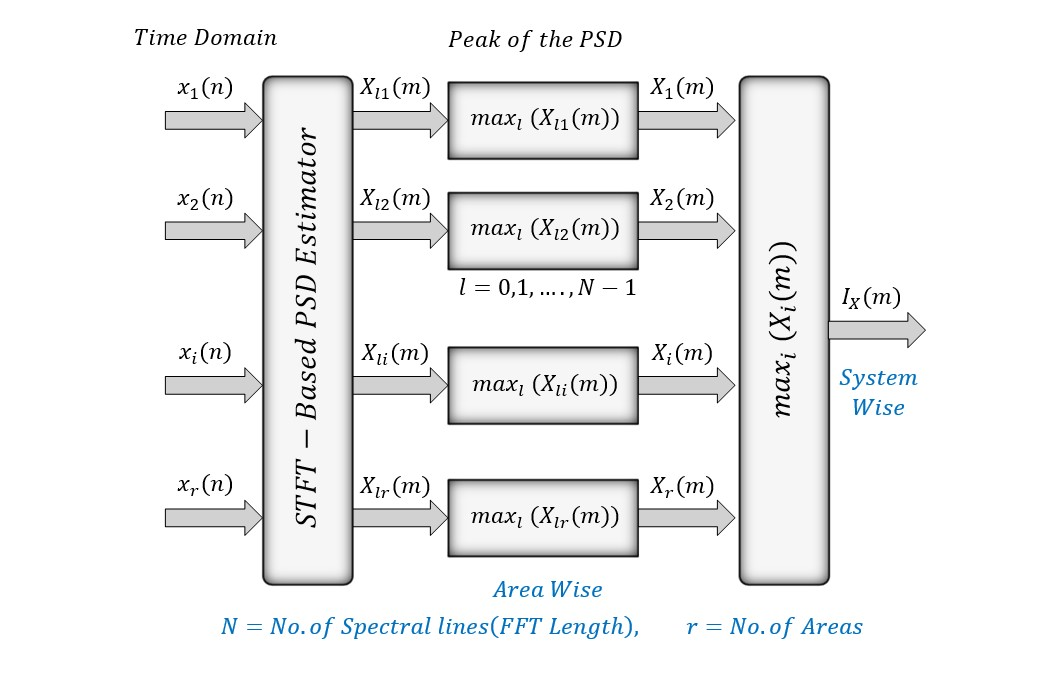
\includegraphics [width=4in] {WASI}
}
\caption{Computation of frequency-domain-based WASI}
\label{fig_WASI}
\end{figure}

\subsection{Inter-area Stability Prediction Index (ISPI)}
\label{ISPI_Intro}
In a network that is interconnected, it is critical to analyse interarea stability in light of grid contingencies. An ISPI is defined \cite{ISPI} in the time domain using two engineering metrics, namely voltage-magnitude change (reduction) and phase-angle movement (separation). This index can be used in place of the previously stated WASI, which is defined in the frequency domain.
\subsubsection{Thresholds values}
By conducting an electrical assessment in the system under consideration, it is able to ascertain angular deviations from ECOI that are vital for the system $\delta cri$, i.e. angular deviations from ECOI which can carry the system nearer to blackout when it is attained, and the maximum angular variations from ECOI that would not affect the system $\delta norm$. The thresholds can be calculated using a contingencies assessment, and they must be perfectly alright to ensure that the algorithm performs consistently in a range of cases..\par

The minimal voltage magnitude allowed $V_{min}$ during transient events, on the other hand, is normally determined by system operator restrictions. For example, voltage level in Colombia's electrical system cannot be less than 0.8 p.u. for more than 500 ms in major buses and 700 ms in the remaining of system \cite{CSA_WASI}.

\subsubsection{Reference Values, Deviation Percent}
A reference must be defined to standardize each parameter.

\begin{equation}
    \Delta V_{ref} = 1 - V_{min}
\end{equation}
\begin{equation}
    V'_{ref} = \frac{\Delta V_{ref}}{\Delta t}
\end{equation}
\begin{equation}
    \Delta d \delta gc_{ref} = \delta cri - \delta norm
\end{equation}
\begin{equation}
    d \delta gc'_{ref} = \frac{\Delta d \delta gc_{ref} }{\Delta t}
\end{equation}

The deviation percent is computed by dividing the variable derived with PMUs by the reference variables, as shown below.

\begin{equation}
    P\Delta V = \frac{\Delta V}{\Delta V_{ref}}
\end{equation}
\begin{equation}
    PV' = \frac{V'}{V'_{ref}}
\end{equation}
\begin{equation}
    P\Delta d \delta gc = \frac{\Delta d \delta gc}{\Delta d \delta gc_{ref}}
\end{equation}
\begin{equation}
    Pd \delta gc' = \frac{ d \delta gc'}{ d \delta gc'_{ref}}
\end{equation}

After normalisation, the percentage variations take values between 0 and one 1. Lastly, the SPI must aggregate four deviations so that the end outcome shows a deviation growth. As a result, we propose the following expression:

\begin{equation}
    SPI = 1-(1-P\Delta V).(1-PV').(1-P\Delta d \delta gc).(1-Pd \delta gc') \label{IL}
\end{equation}
Normal, alert, and alarm are the three different states of the system (Fig. \ref{ISPI Categories}). So because SPI index is standardized, the restricting level can also be set to 100\%, which implies the normal condition can be set to the less than 33\%, the alert state to 33\% to 66\%, and the alarm state to more than 66\%. These changeover levels among normal, alert, and alarm can be easily changed when building the off-line stress level collection from power-flow studies. sO, Categories of the ISPI can be as follows.

\begin{figure}[H]
	 \centering
	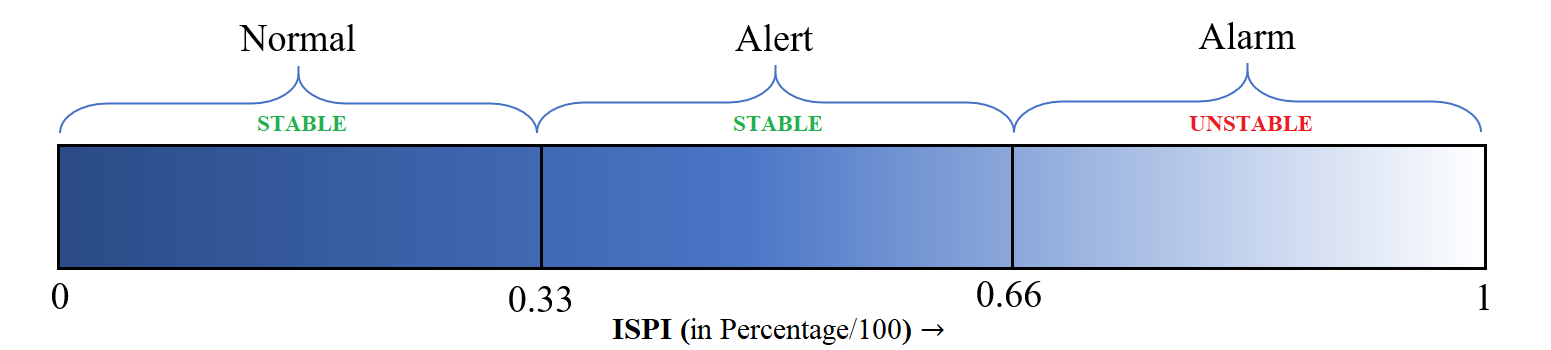
\includegraphics[width=12 cm]{ISPI Categories.png}
	\caption{Stability Prediction Index Categories}
	\label{ISPI Categories}
	\end{figure}

\section{Problem Formulation}
A power system is made up of a few basic components that are all interrelated. The generators, transmission lines, loads, transformer, static VAR compensators, and HVDC lines are the most important. There might be a couple of disturbances during the activity of the generators, for example, upheld movements in the speed or intermittent varieties in the force applied to the generator. These annoyances may cause a change in voltage or frequency, which may affect various components of the interconnected power system. Lightning and other external elements can also wreak havoc on the power system and transfer capacity between frameworks. Faults is the name given to this slew of disquieting influences. If the typical frequency of oscillation harmonises with the frequency oscillation of the generators, an fault causes the motor to lose synchronism. In light of these factors, synchronism is a necessary requirement for a power system with stability. Other crucial variables include steady-state stability, transient stability, music and unsettling impact, voltage breakdown, and a lack of reactive power, among others. The ability of an interconnected power system to return to its generally expected or stable activity after being subjected to some sort of adversity. Framework stability is defined as the ability of the framework to provide the heap and keep the many synchronous machines in sync under various conditions without the assistance of anybody else. The investigations are helpful in determining things like why a need has emerged. Voltage level, critical clearing time of circuit breakers. So, proposed methods of evaluating system is by considering Catastrophic Indicator computation and to take necessary steps looking at stability of the system in due time. Importance of the discussed formulas are they are easy and simple and easy to execute once the required parameters are obtained in case of proper Algorithm is there to execute all indicators.  % Problem Formulation
\chapter{Solution Methodology}

\section{Introduction}
 The methodology for online stability prediction is is generalized using a flowchart shown in fig. \ref{Flowchart}. It is a long process but in my paper discussed portion is of only computation of indicators. So left out processes like fault detection, post fault data collection, stability analysis are carried out using MAT-POWER and MAT-TRANS Software. These softwares are discussed in following sections.\par
 After fault occurs the data are collected from PMU and Time-stamped measurements data generated from simulation. Then the data are sent for performing Stability Analysis. The Results are taken out for obtaining different required parameters, one of them is Coherency Referred measures
Computation, that includes Computation of Area Based COI,
System Based COI, then COI. After getting the parameters different Catastrophic Indicators are Computed one by
one to analyze them.
 
 \begin{figure}
	 \centering
	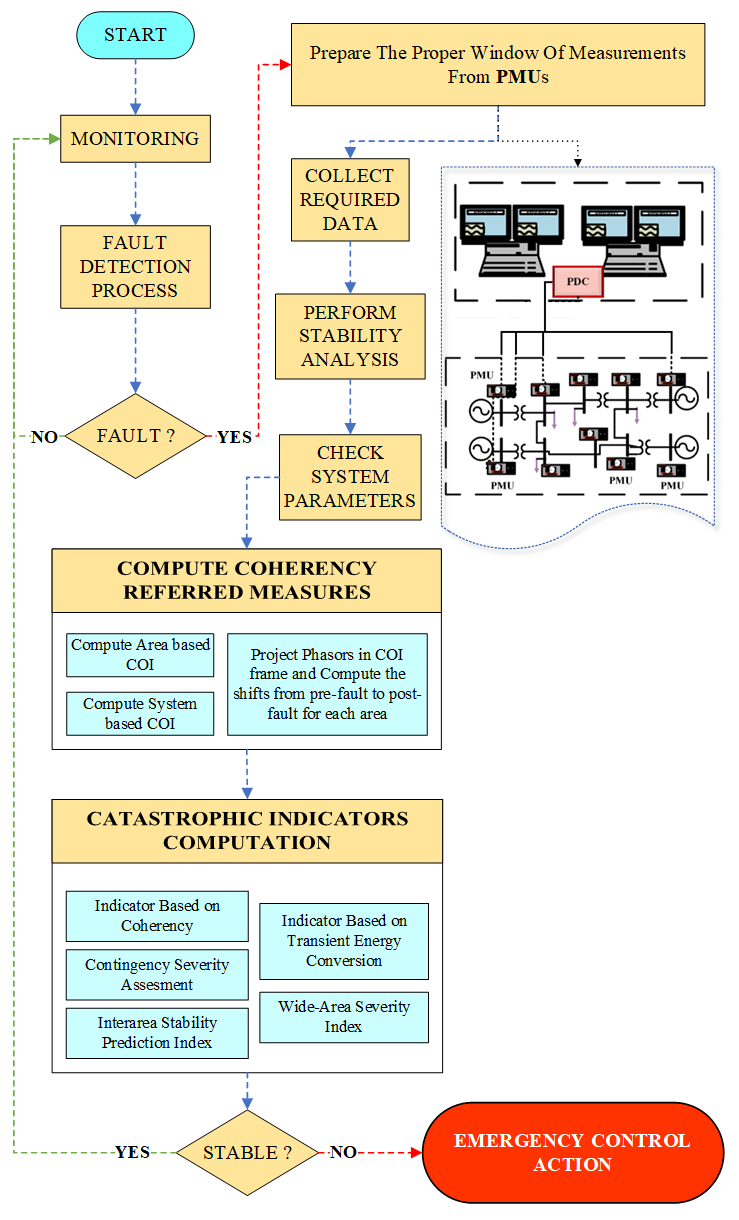
\includegraphics[width=12 cm]{Flowchart2.png}
	\caption{Flowchart of Stability Prediction Procedure}
	\label{Flowchart}
\end{figure} 

\section{MAT-POWER Tool Box}
 This Toolbox provides 59 built-in MATLAB programs for various famous test Systems. All these MATLAB programs of various test systems are shown in the DATA folder of the MAT-POWER toolbox, which can be directly used. It is expected as a simulation device for scientists and teachers that is not difficult to utilize and adjust. MAT-POWER is intended to give the most ideal exhibition while keeping the code easy to comprehend and adjust. Syntax for running the Optimal power Flow of a Case:- \textbf{runopf(‘casefilename’);} A simple example of MAT-POWER use can be described in following sub-section along with its result comparison with theoretical values.

\subsection{Economic Load Dispatch Example on IEEE-9 Bus System}
\begin{itemize} 
\item[\tiny{$\blacksquare$}]The M-file for IEEE-9 Bus test name is case9. So, the syntax for running optimal Power flow or Economic load Dispatch in IEEE-9 Bus system is \textbf{runopf('case9')}. By default it will perform the optimal power flow using MATPOWER Interior Point Solver(MIPS). 
\item[\tiny{$\blacksquare$}]It has taken the computational time of 3.06 seconds. Furthermore, the total minimum cost to supply the load of IEEE-9 Bus system is 5296.69 \$/hr. It further shows the important results of IEEE-9 bus system such as minimum and maximum voltage magnitudes, Voltage angle, active and reactive power loss and incremental fuel cost. Along with Total Power Supplied, Total Power Demand and Total Loss is also generated as 318.31 MW, 315.0 MW and 3.31 MW respectively.
\item[\tiny{$\blacksquare$}]The Mat-Power software testing is completed with Results and are compared and verified to be same as the Theoretical data.
\end{itemize}
\textbf{*Although there is no direct use of MAT-POWER Software, but the later proceedings need the presence of it along with MATLAB.}

\section{MAT-TRANS Software}
MATTRANS is a MATLAB(R)/Simulink (M-files and.mdl files) programme for transient stability analysis. It's a free and open-source programme. It's designed to be a simple to use and modify simulation tool for researchers and instructors. MATTRANS was created with the goal of providing the highest feasible performance while making the code simple to understand and modify. It was first created in 2008, and the files are available at\cite{MattransSoft}. In MATTRANS, the runts(case\#, case\#dd) function requires two.m input files. There are two types of network data: 1) steady-state data and 2) dynamic data. The network steady-state data format is identical to that of MATPOWER \cite{L1}, but the network dynamic data format contains variables for generator machines, exciters, turbines, and power system stability.

\subsection{Pseudo-Code of the MATTRANS Software}
This software Runs a Transient Stability. Where, mpc = 
runts(casedata, mpopt, fname, solvedcase). It runs a 
Transient Stability (First executes power flow then simulate transtability.mdl), returning results. Its software coading includes following steps-
\begin{enumerate}
\item Imports code files such as “import +data.*; import +exciter.*; import +generator.*; import +load.*; import +pss.*; import +turbine.*; import +utils.*; import +Yform.*; “ to include exciter data, generator data, load data and other important data’s with functions to carryout important logics for transient stability analysis.
\item Initializes named Indices for bus, generator and branch matrices.
\item	Executes steady-state power flow. moption used to set and retrieve a MATPOWER option structure runpf runs a power flow.
\item	Adding dynamic data to the mpc structure and adding extra variables but gen, order variables are removed from mpc as they are already included in the Simulink file.
\item	Generator variables for a particular case data is included.
\item	Exciter variables are initialized and they are enabled or disabled according to corresponding generator.
\item	Turbine and speed governors values are initialized and they are enabled or disabled according to corresponding generator.
\item	Initialization of PSS Models and they are enabled or disabled according to the corresponding generators. This process includes initialization of PSS Models, selectors for individual type of PSS, Indication of the generator number of which specific type of PSS is to be enabled otherwise it is marked as zero and then wrapping up it into a single structure.
\item	Modelling Load variables include finding load variables and wrapping up it into a single structure to reduce complexity.
\item	Modelling Y-Bus w.r.t line trips includes necessary variable declaration, Y-bus formation, inclusion of dynamic data of both load and generator in Y-bus, input command line interface for users to enter fault data followed by condition for tripping of lines to clear fault and wrapping all data’s into a single structure.
\item	Execution of transientStability.mdl i.e. a Simulink file specially used for evaluation of above collected datas and shows parameter output for the indicators for assessment of stability.
\end{enumerate}

\subsection{Simulation Models}
Execution of transientStability.mdl includes the execution of the base model known as \textbf{Transient Stability model} shown in Fig. \ref{TSM} which also includes various sub models to check for Transient Stability of a system. Important sub models are \textbf{Generator, Turbine System, Excitation system, Power System Stability Model, Static Loads and its outputs}, which are discussed below. 
\begin{figure}[H]
	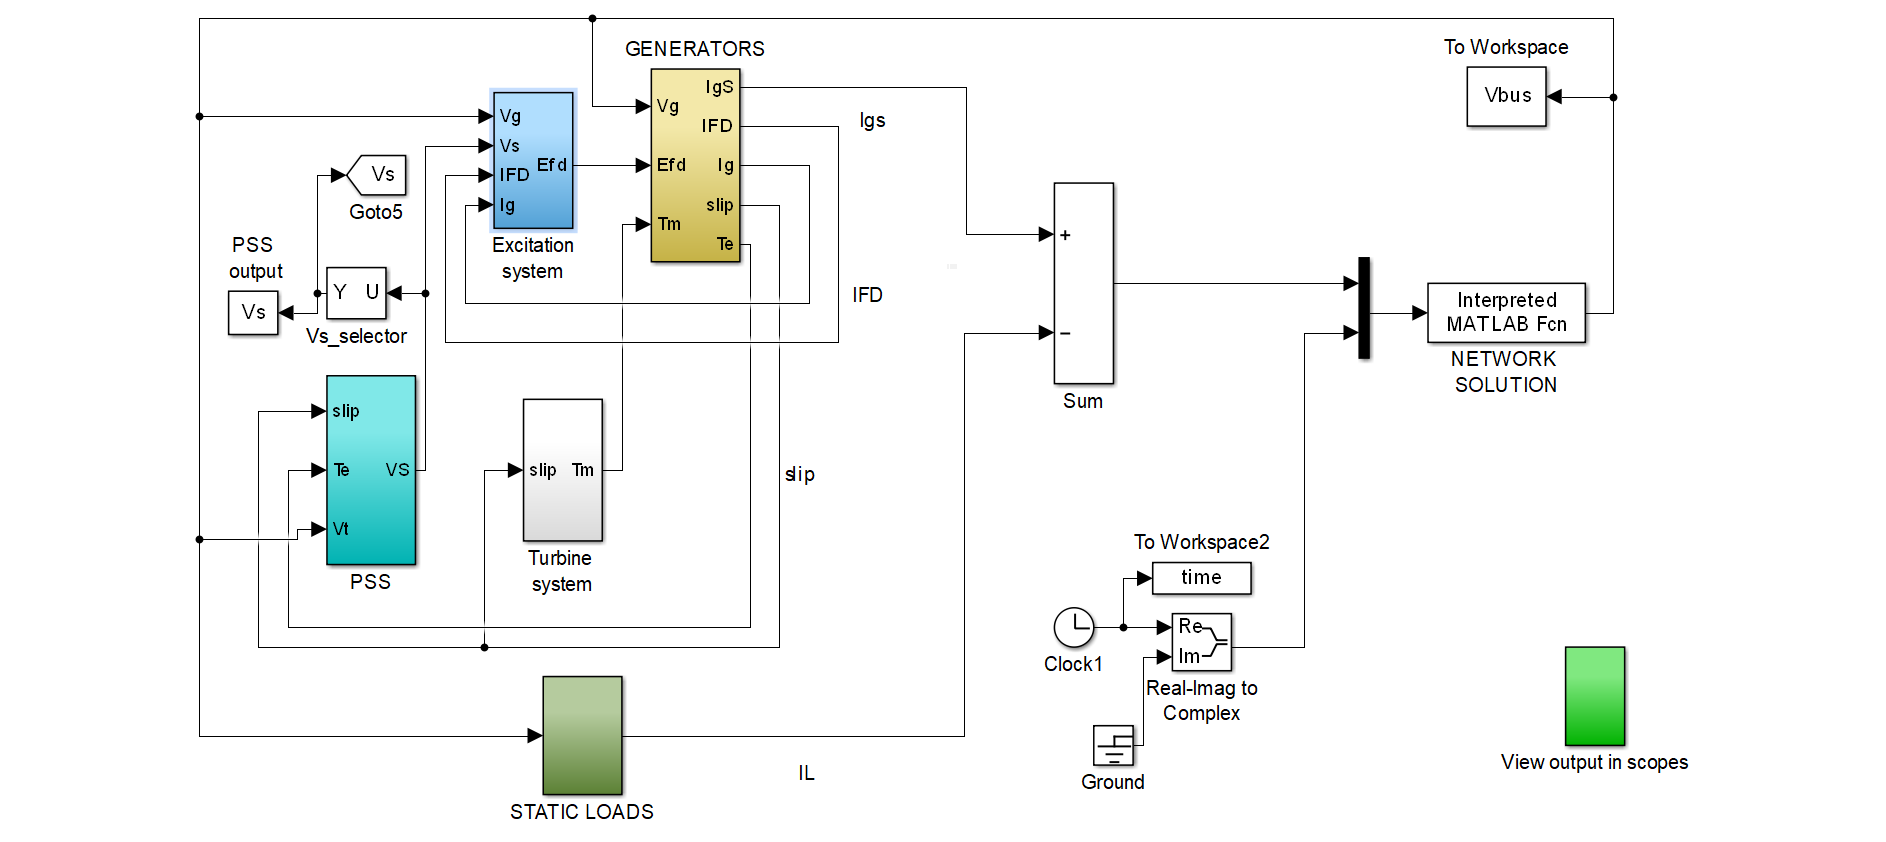
\includegraphics[scale=0.4]{Transient Stability}
	\caption{Transient Stability Model}
	\label{TSM}
	\end{figure}
	
\begin{enumerate}
%% 1. Generator Model==============================================================
\item \textbf{\large Generator Model}: It is created to do the work of a normal generator (Electric machine) shown in Fig. \ref{GM} and along with calculating its parameters like torque, angle deviation, field current, saliency etc..
	
	\begin{figure}[H]
	 \centering
	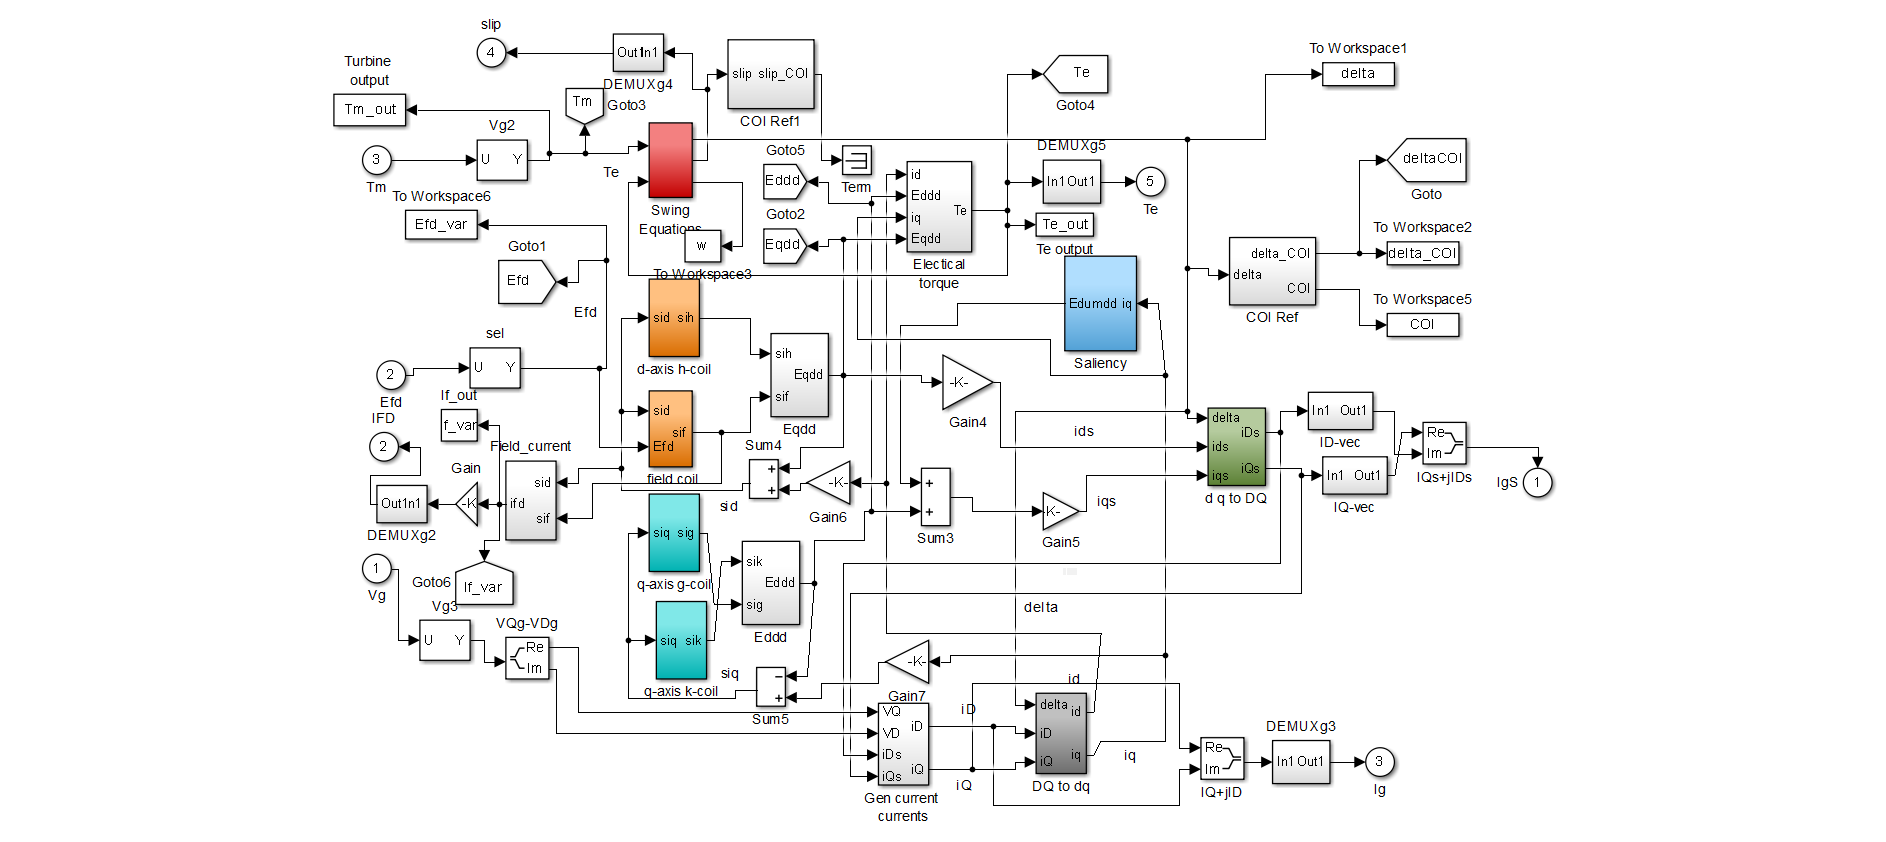
\includegraphics[scale=0.4]{Generators}
	\caption{Generator Model}
	\label{GM}
	\end{figure}
	% Generator Sub models-------------------------------------------------------
	\begin{itemize}
%		\item \textbf{\large Generator Sub Models}: Generator parts like Field Coil 			parameters, Direct axis parameters, Quadrature axis parameters, Saliency 				models are prepared for making a complete generator model and for 					calculating generator parameters and also COI Reference Model for obtaining 			generator speed Deviation.
%		\begin{figure}[H]
%		 \centering
%		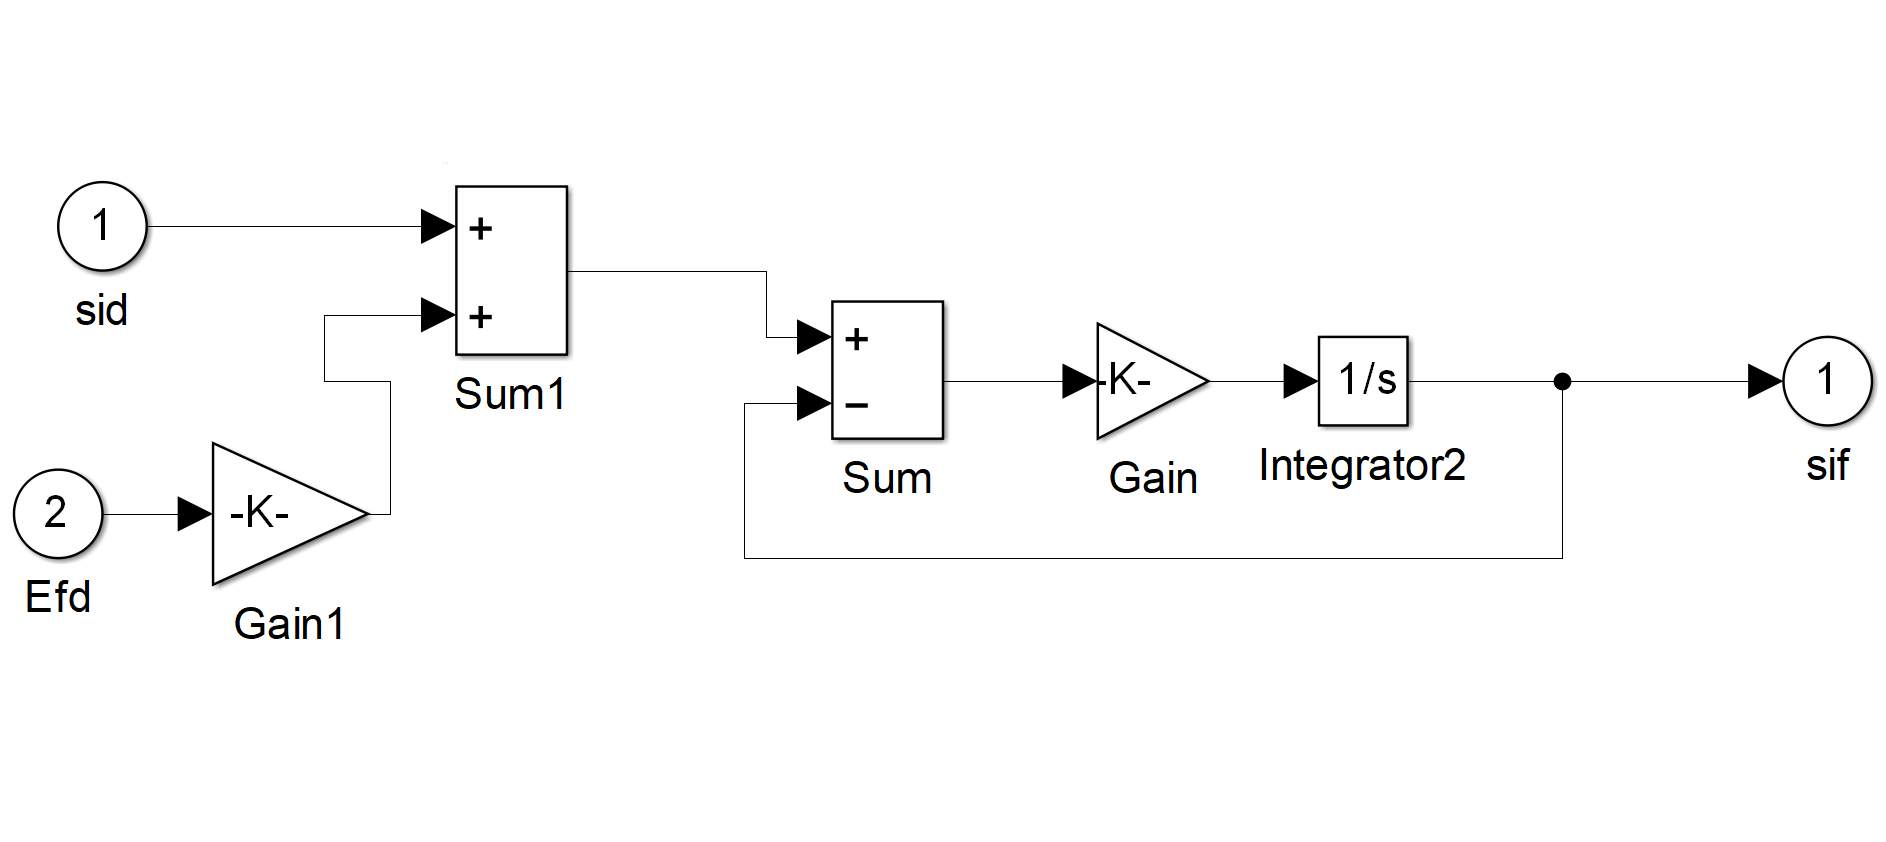
\includegraphics[scale=0.3]{Field Coil}
%		\caption{Field Coil Model}
%		\label{Field Coil}
%		\end{figure}
%		
%		\begin{figure}[H]
%		 \centering
%		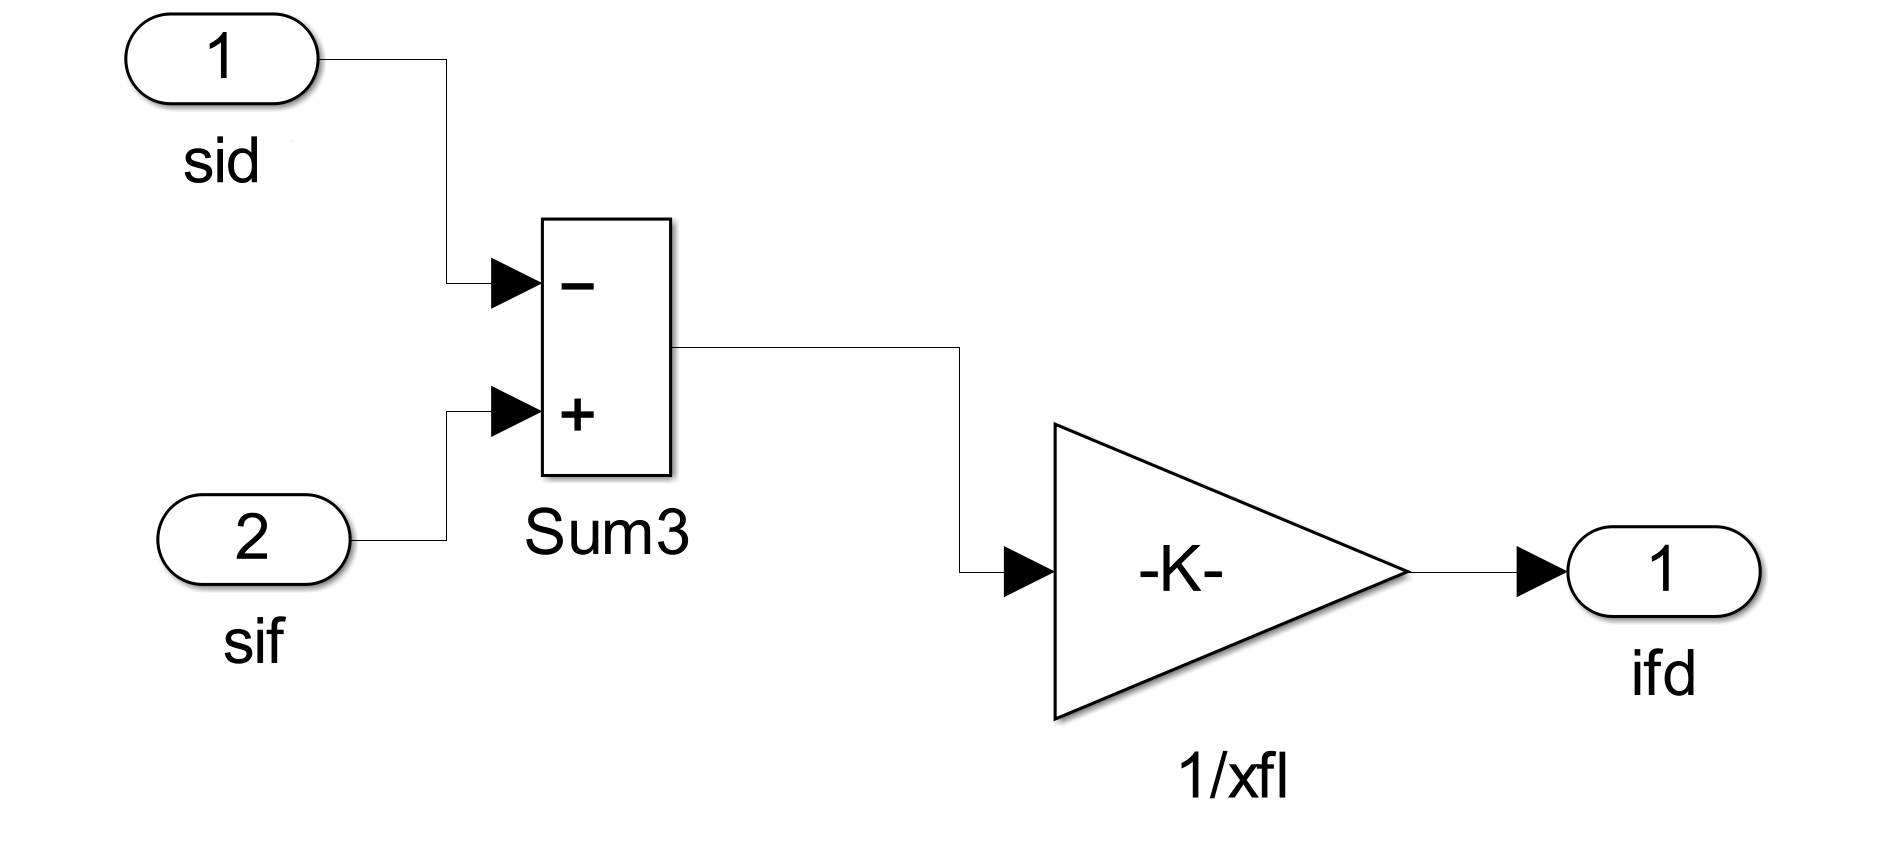
\includegraphics[scale=0.3]{Field Current}
%		\caption{Field Current Model}
%		\label{Field Current}
%		\end{figure}
%		
%		\begin{figure}[H]
%		 \centering
%		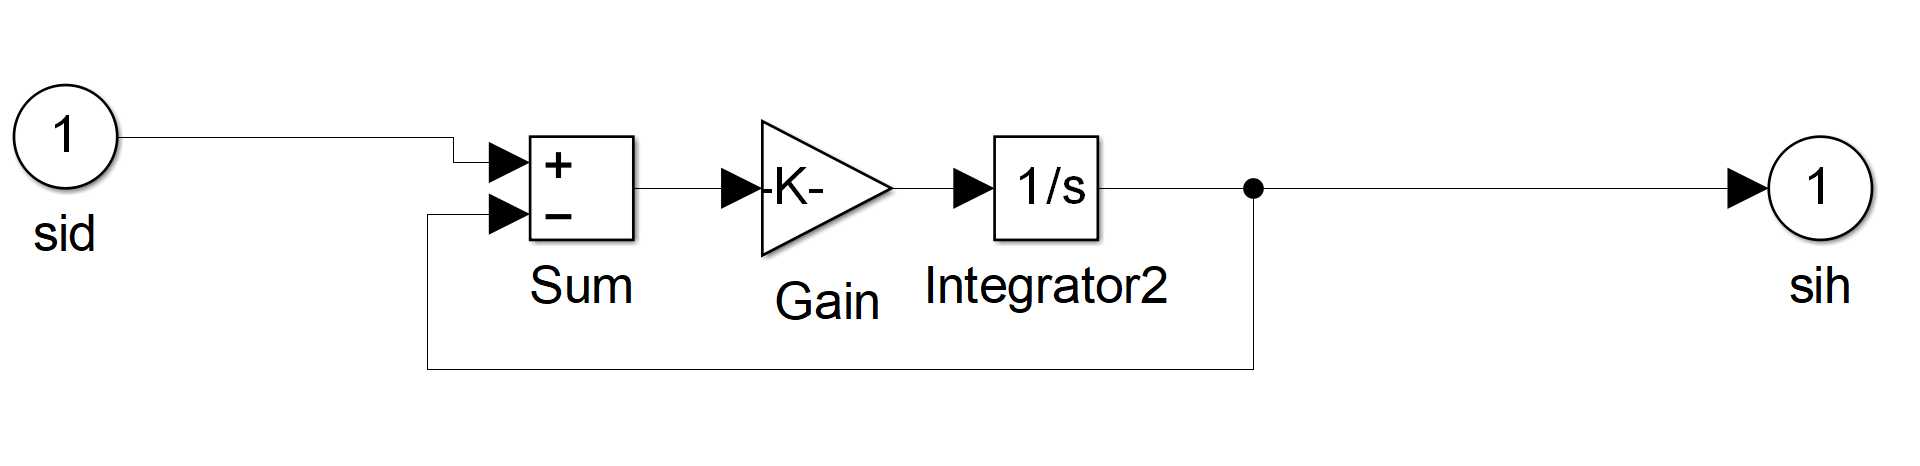
\includegraphics[scale=0.3]{d-axis h-coil}
%		\caption{d-axis h-coil Model}
%		\label{dh}
%		\end{figure}
%		
%		\begin{figure}[H]
%		 \centering
%		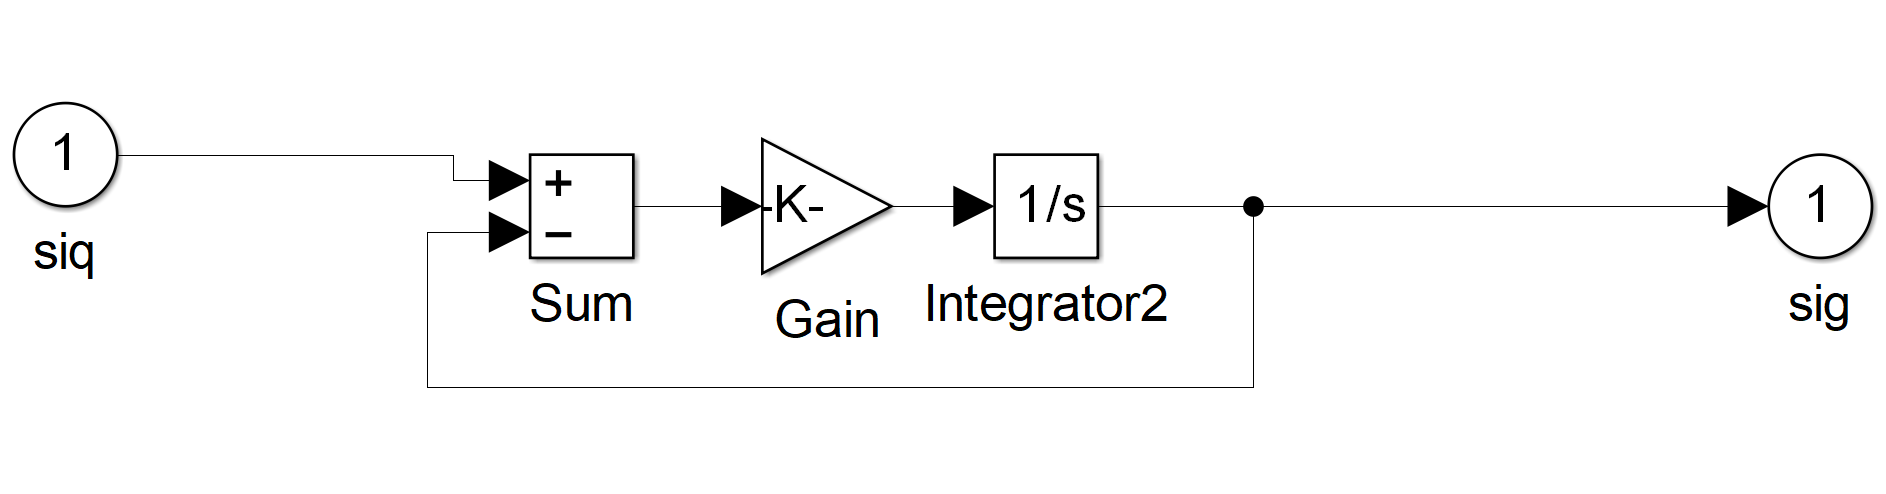
\includegraphics[scale=0.3]{q-axis g-coil}
%		\caption{q-axis g-coil Model}
%		\label{qh}
%		\end{figure}
%		
%		\begin{figure}[H]
%		 \centering
%		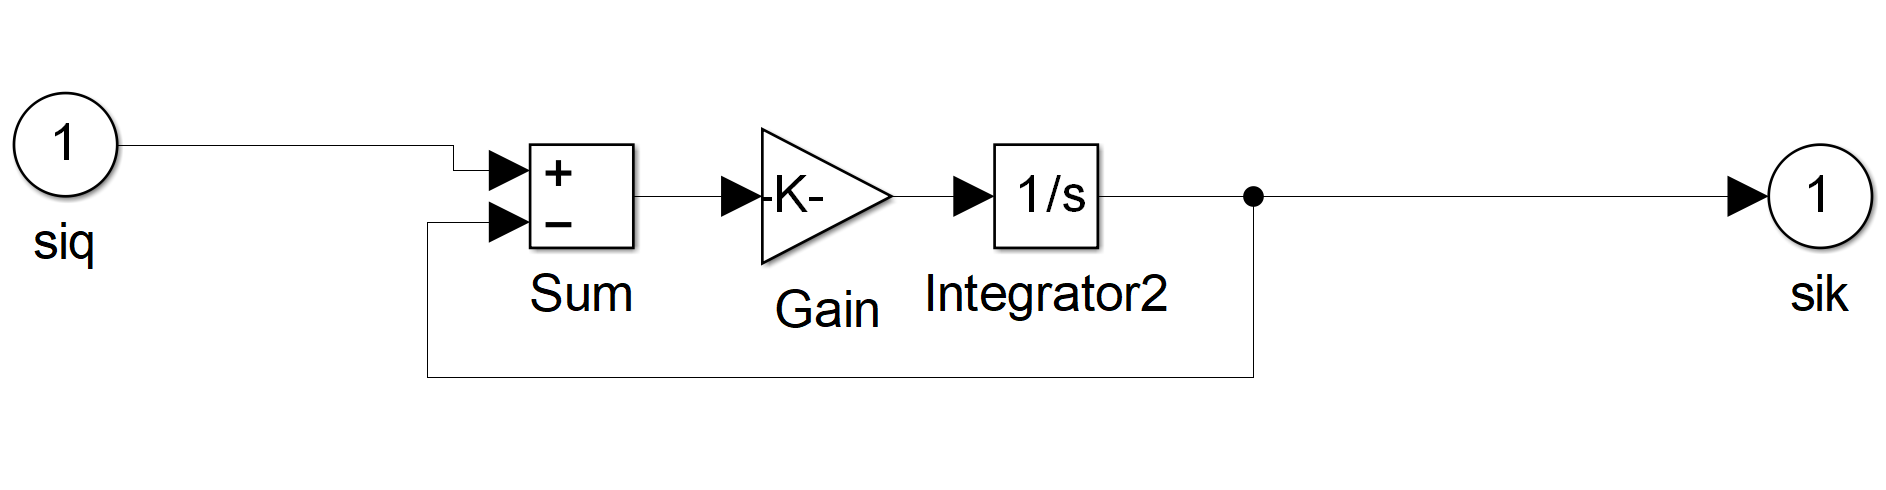
\includegraphics[scale=0.3]{q-axis k-coil}
%		\caption{q-axis k-coil Model}
%		\label{qk}
%		\end{figure}
%		
%		\begin{figure}[H]
%		 \centering
%		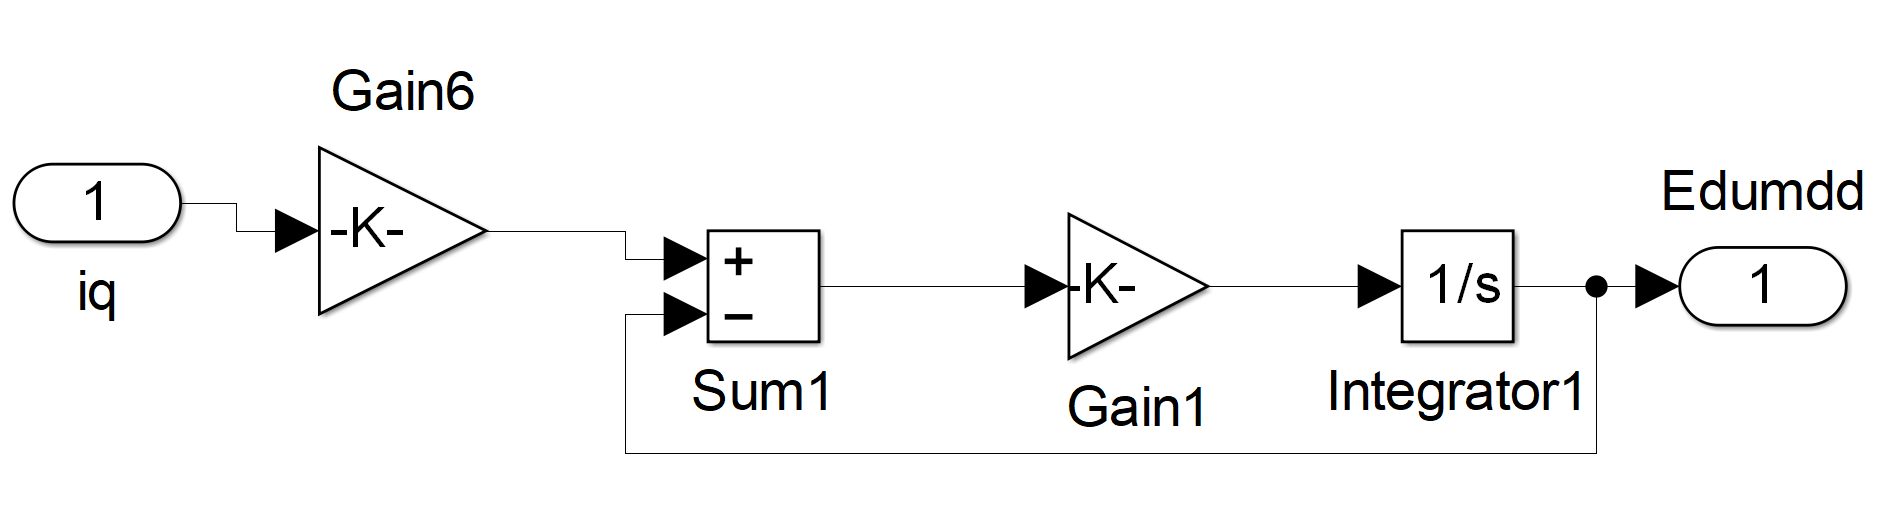
\includegraphics[scale=0.3]{Saliency}
%		\caption{Saliency Model}
%		\label{Saliency}
%		\end{figure}
%		
%		\begin{figure}[H]
%		 \centering
%		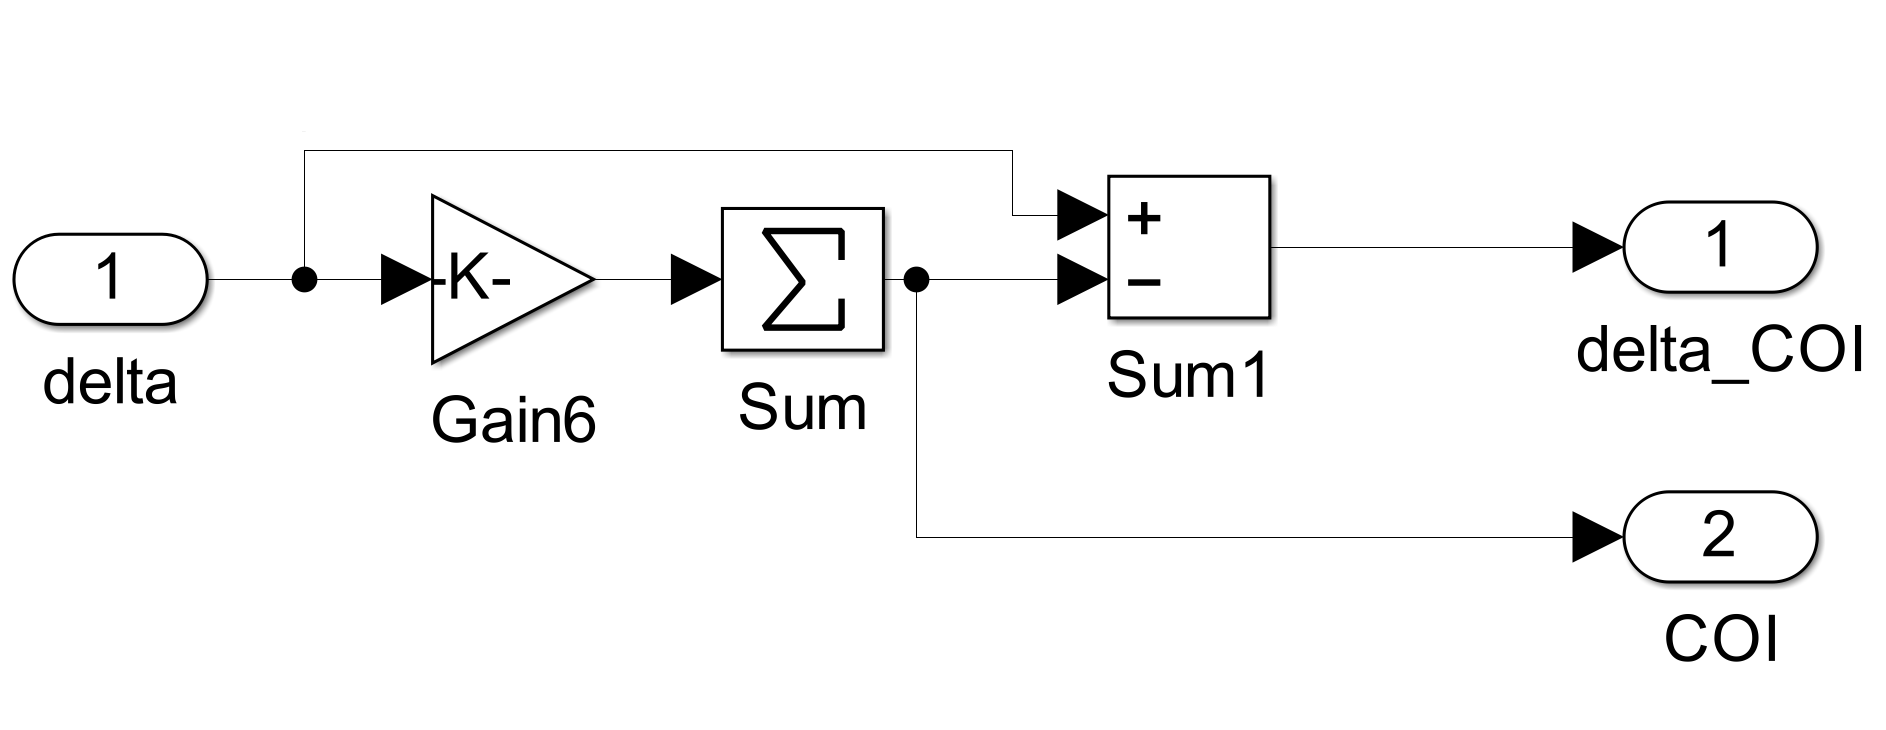
\includegraphics[scale=0.3]{COI Ref}
%		\caption{COI Ref Model}
%		\label{COI Ref}
%		\end{figure}
%		
%		\begin{figure}[H]
%		 \centering
%		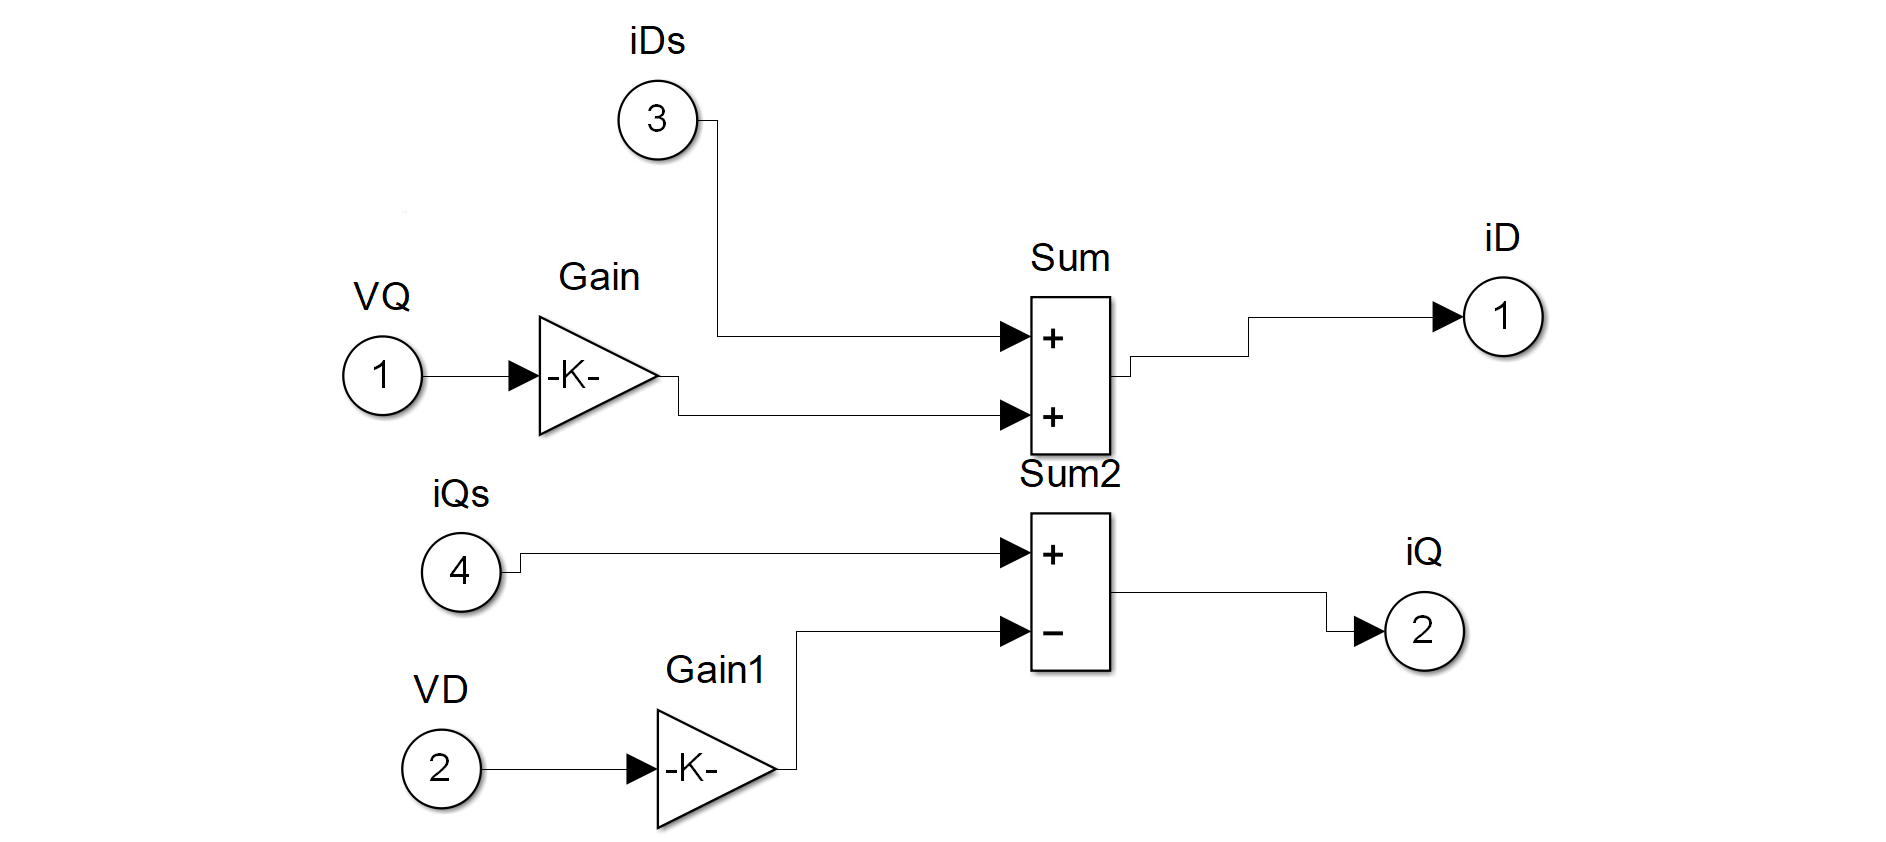
\includegraphics[scale=0.4]{Generator Current}
%		\caption{Generator Currents Model}
%		\label{Generator Current}
%		\end{figure}
		
		\item \textbf{\large Swing Equation Model}: The model shown in Fig. \ref{swing eqn} is for the equation governing the motion of the rotor of a synchronous machine as described previously in Section-2.1 .
		\begin{equation}
		J\frac{d^2\theta_m}{{d(t)}^2}= T_a = T_m - T_e
		\end{equation}
		\begin{figure}[H]
		 \centering
		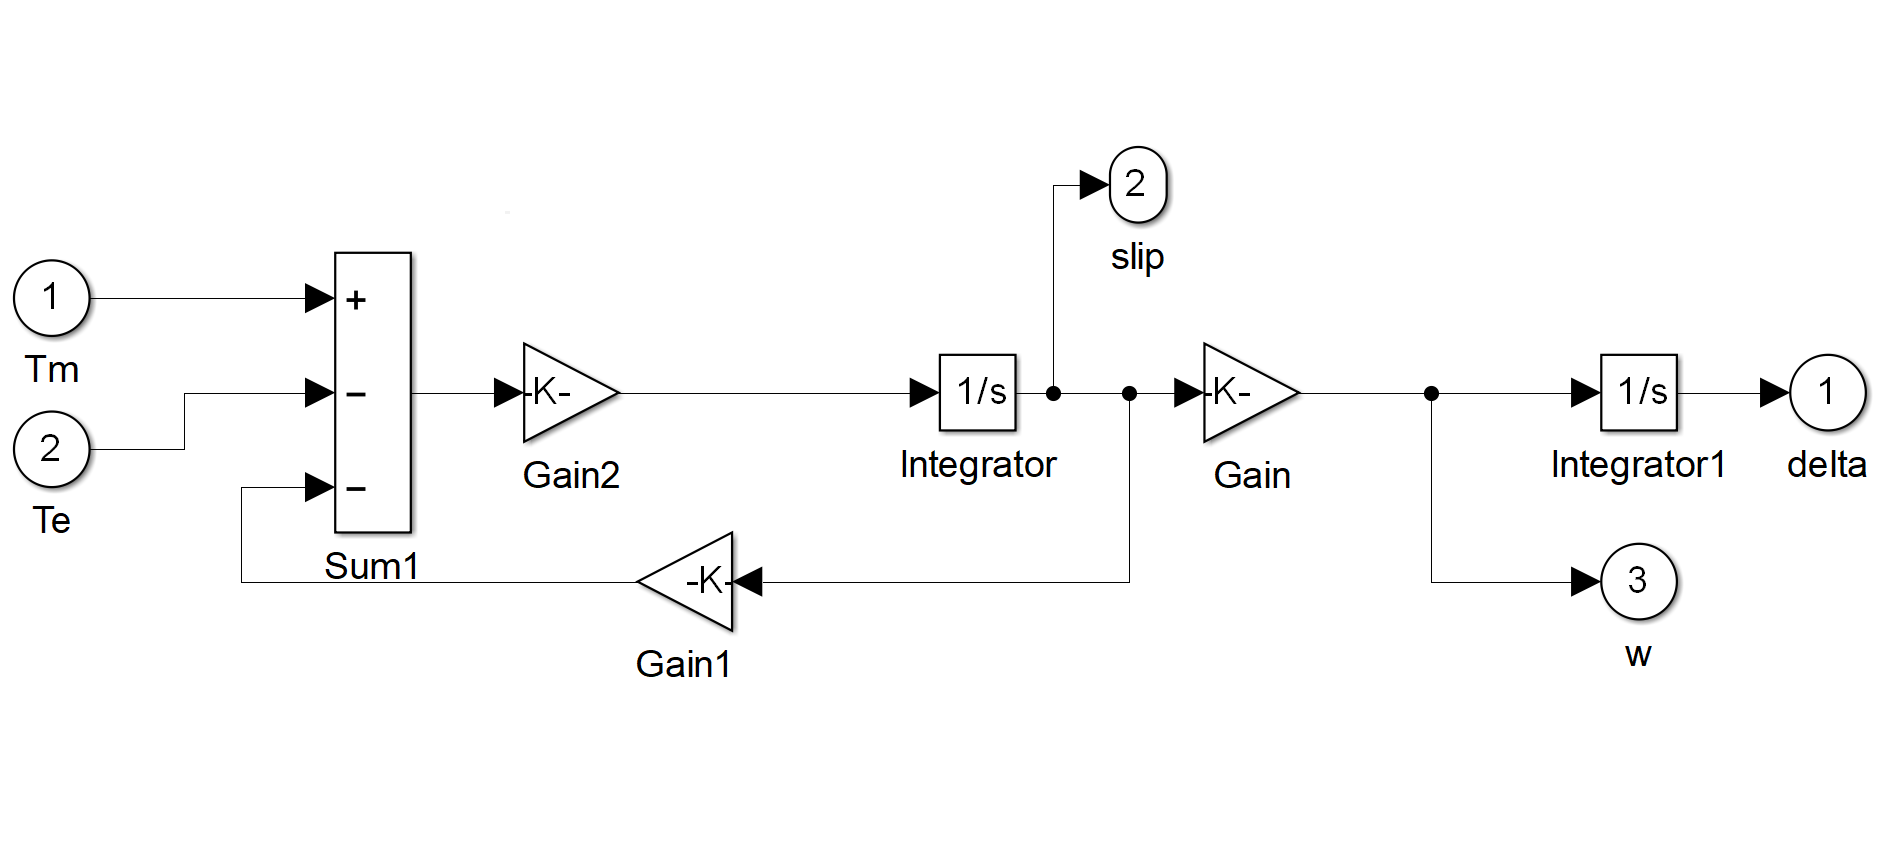
\includegraphics[scale=0.3]{swing eqn}
		\caption{Swing Equation Model}
		\label{swing eqn}
		\end{figure}
		
%		\item \textbf{\large Electric Torque Model}: This is the sub model for creating electric torque from direct axis and quadrature axis current and voltage.
%		\begin{figure}[H]
%		 \centering
%		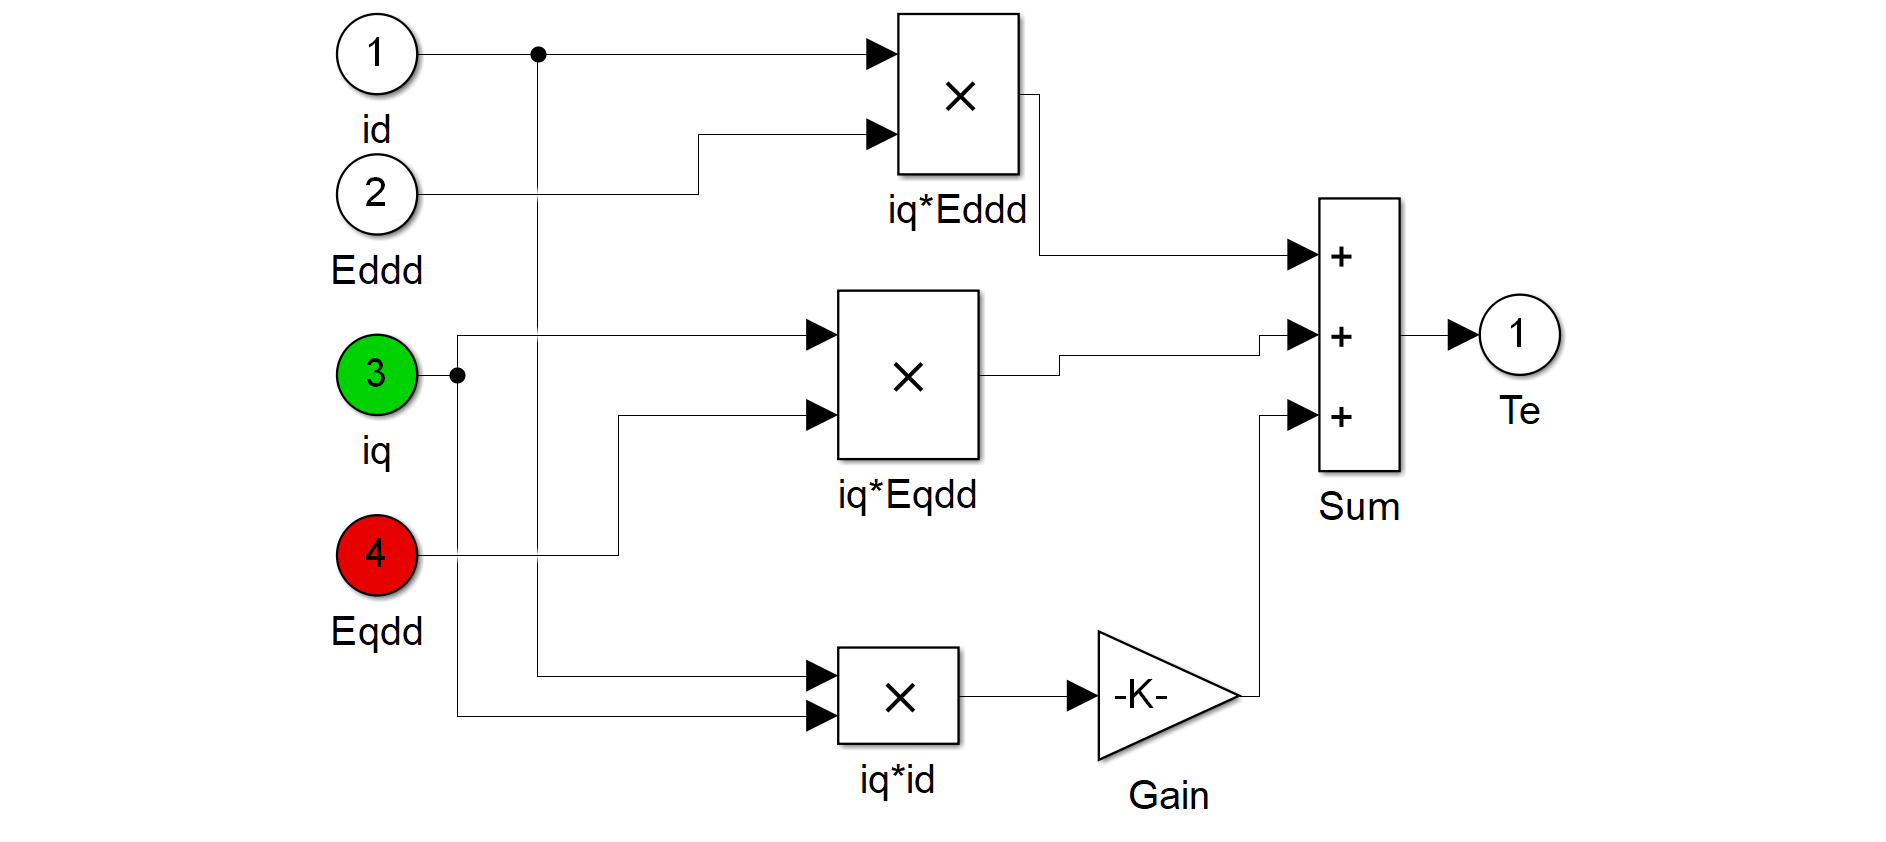
\includegraphics[scale=0.4]{Electric Torque Model}
%		\caption{Electric Torque Model}
%		\label{Electric Torque Model}
%		\end{figure}
%	%	
%	%	\begin{figure}[H]
%	%	 \centering
%	%	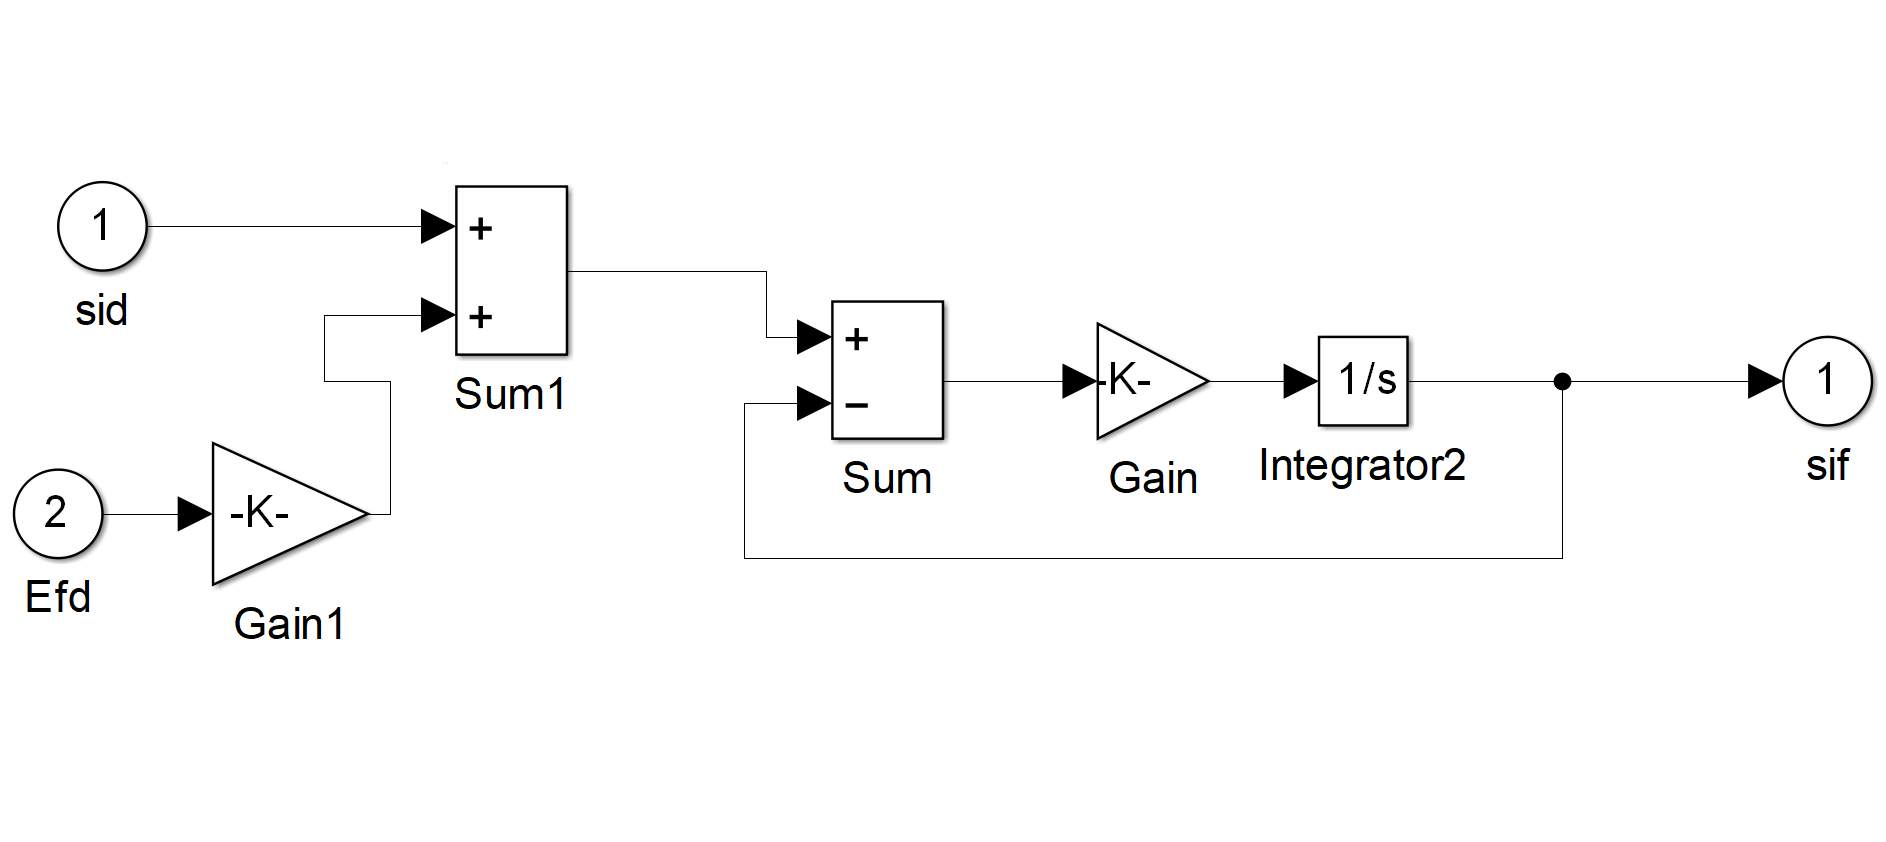
\includegraphics[scale=0.4]{Field Coil}
%	%	\caption{Field Coil}
%	%	\label{Field Coil}
%	%	\end{figure}
	\end{itemize}
%% 2. Turbine System Model =========================================================	
\item \textbf{\large Turbine System Model}: Different Turbine Systems are included such as Speed Governor Hydro Turbine, Speed Governor Reheat Steam turbine and Non Reheat Steam turbine to add Turbine parameters to check system variance in case of real time use.
	
	\begin{figure}[H]
	 \centering
	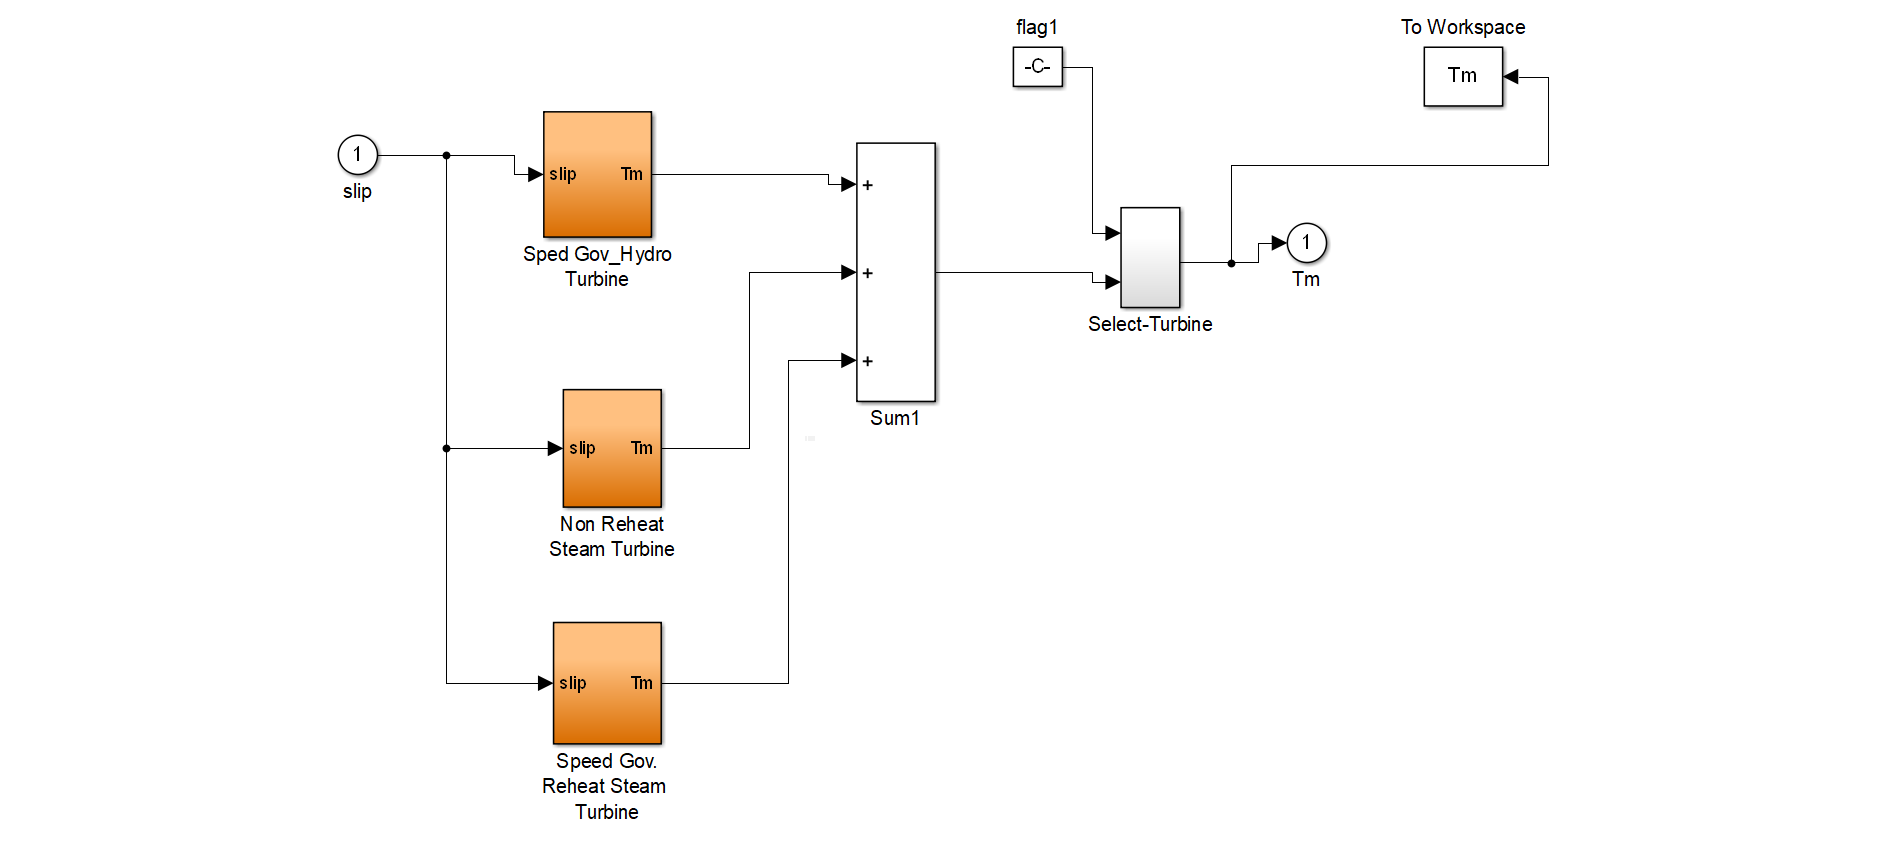
\includegraphics[scale=0.4]{Turbine}
	\caption{Turbine System Model}
	\label{Turbine System Model}
	\end{figure}
	
%	% Turbine System Sub Models-------------------------------------------------
%	\begin{itemize}
%	\item \textbf{\large Turbine System Sub Models}: Three turbine systems are used for a basic generator as follows.
%		\begin{figure}[H]
%		 \centering
%		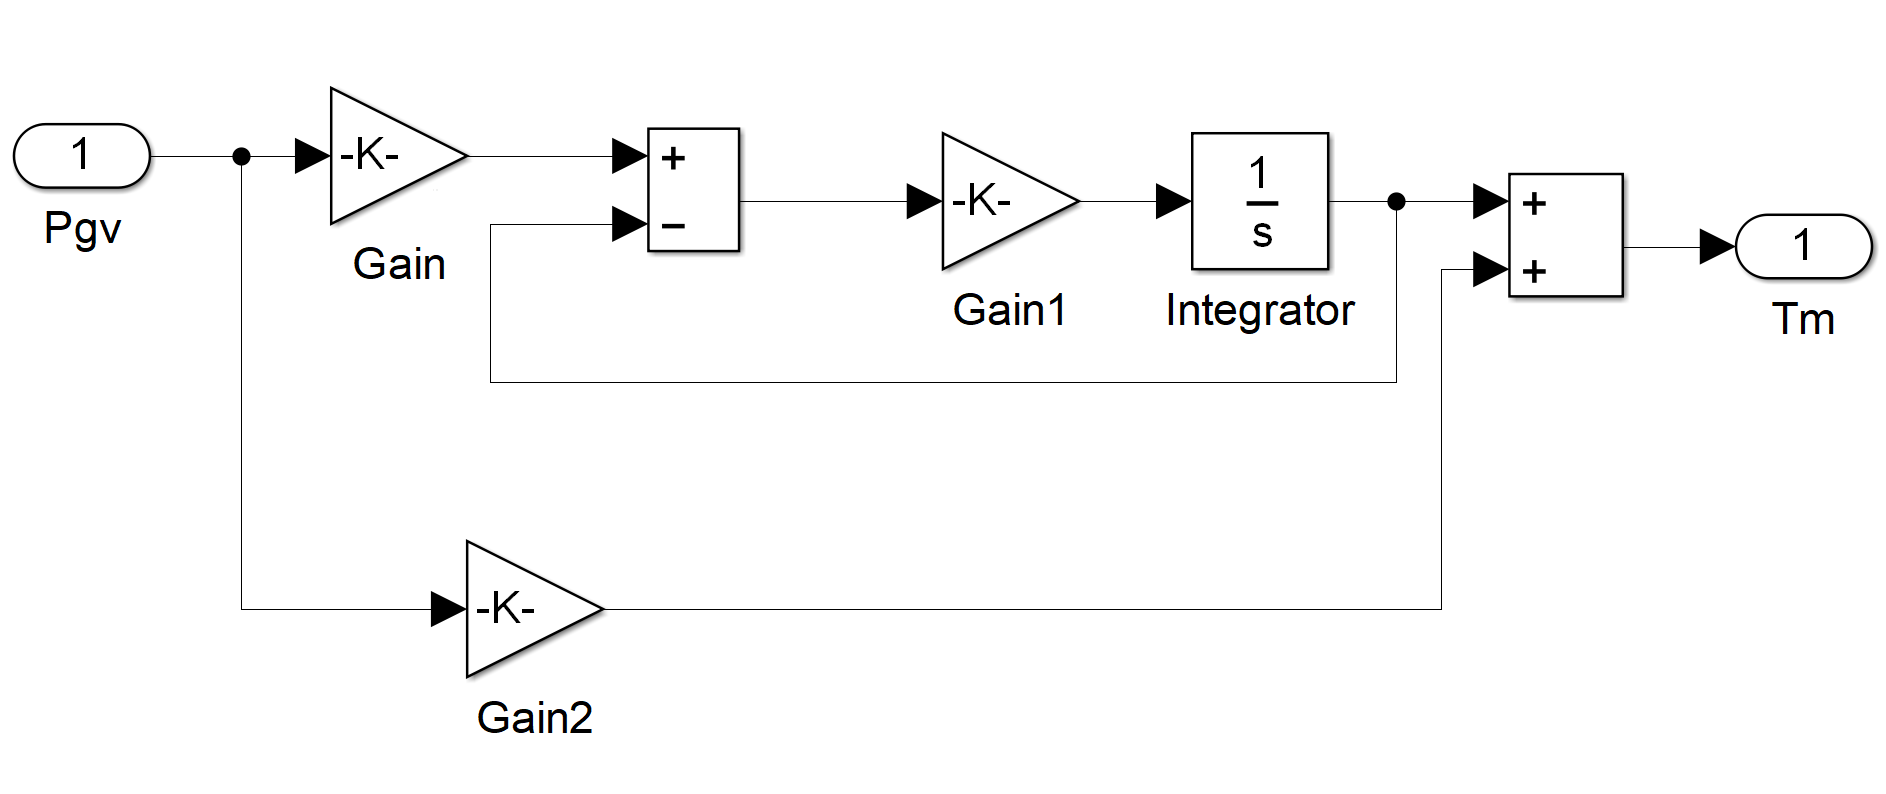
\includegraphics[scale=0.3]{Hydro Turbine Model}
%		\caption{Hydro Turbine Model}
%		\label{Hydro Turbine Model}
%		\end{figure}
%		
%		\begin{figure}[H]
%		 \centering
%		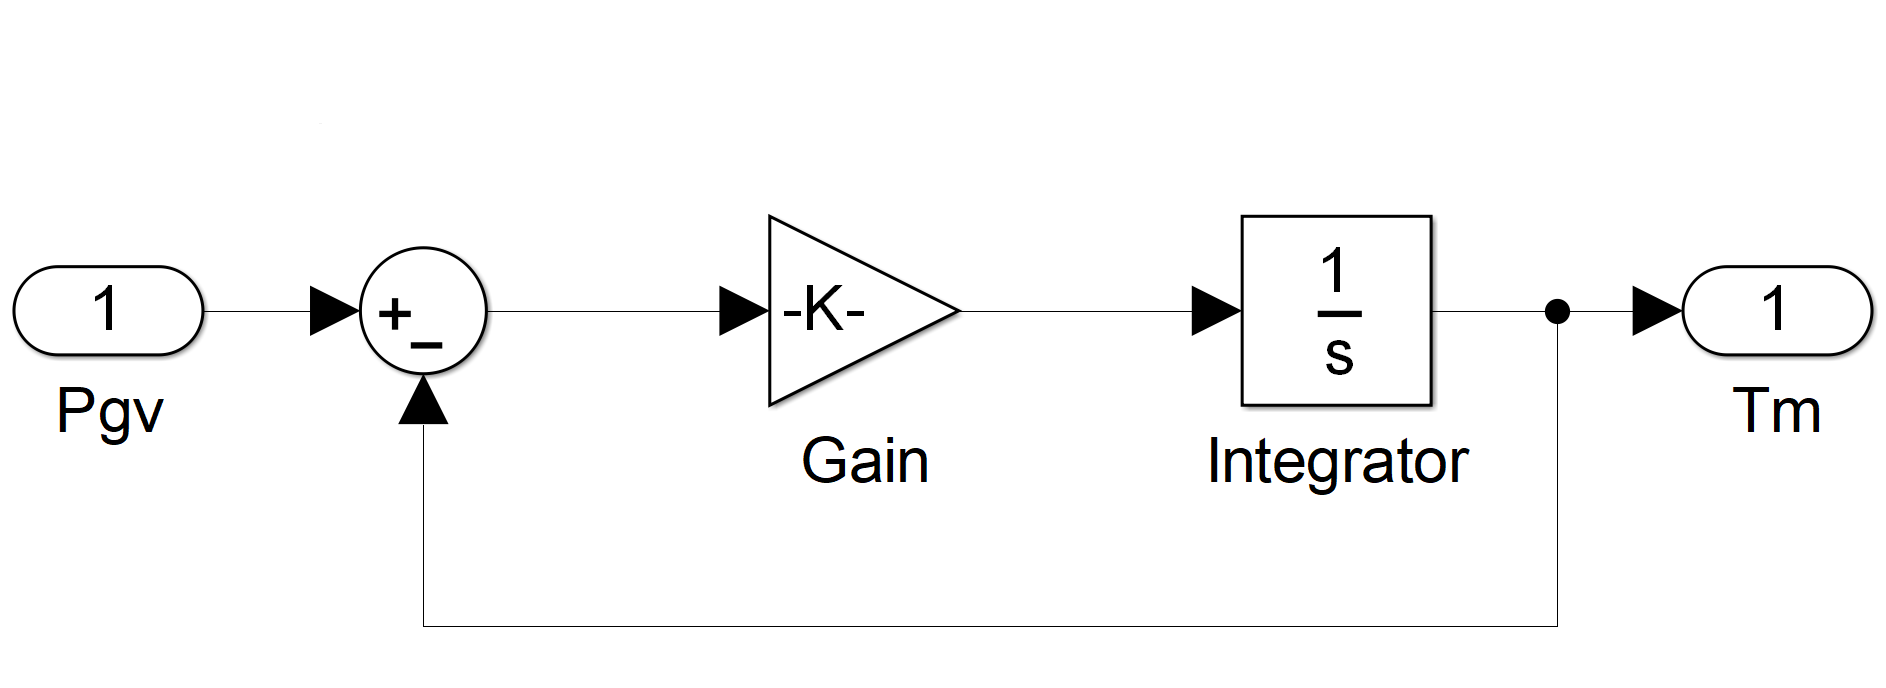
\includegraphics[scale=0.3]{Non Reheat Turbine}
%		\caption{Non Reheat Turbine}
%		\label{Non Reheat Turbine}
%		\end{figure}
%		
%		\begin{figure}[H]
%		 \centering
%		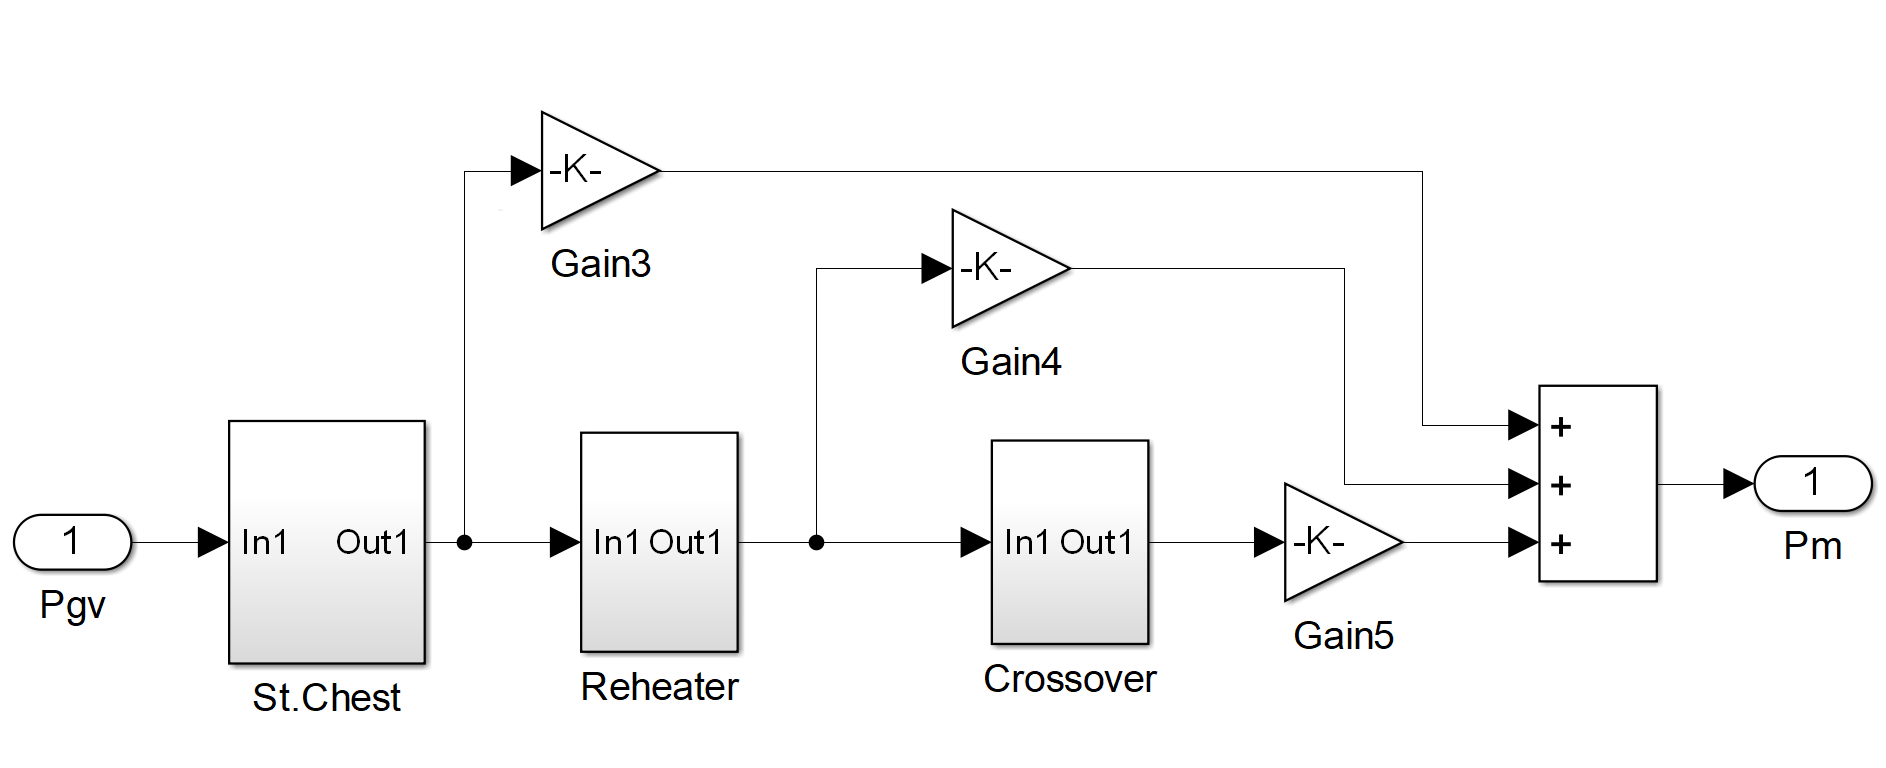
\includegraphics[scale=0.3]{Reheat Turbine}
%		\caption{Reheat Turbine}
%		\label{COI Ref}
%		\end{figure}
%		
%				
%	\item \textbf{\large Turbine Governor System Models}: Turbine governor systems are used for a basic generator as follows.
%		\begin{figure}[H]
%		 \centering
%		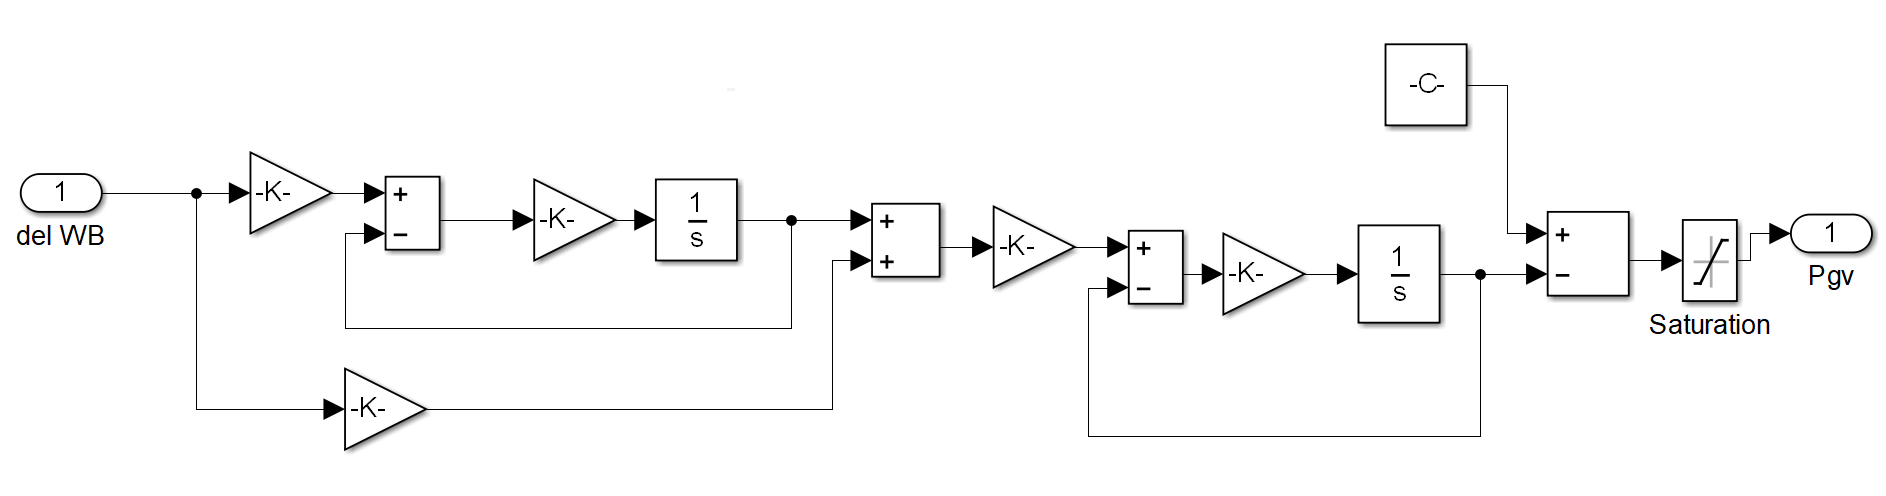
\includegraphics[scale=0.3]{Governor model}
%		\caption{Governor model}
%		\label{Governor model}
%		\end{figure}
%				
%		\begin{figure}[H]
%		 \centering
%		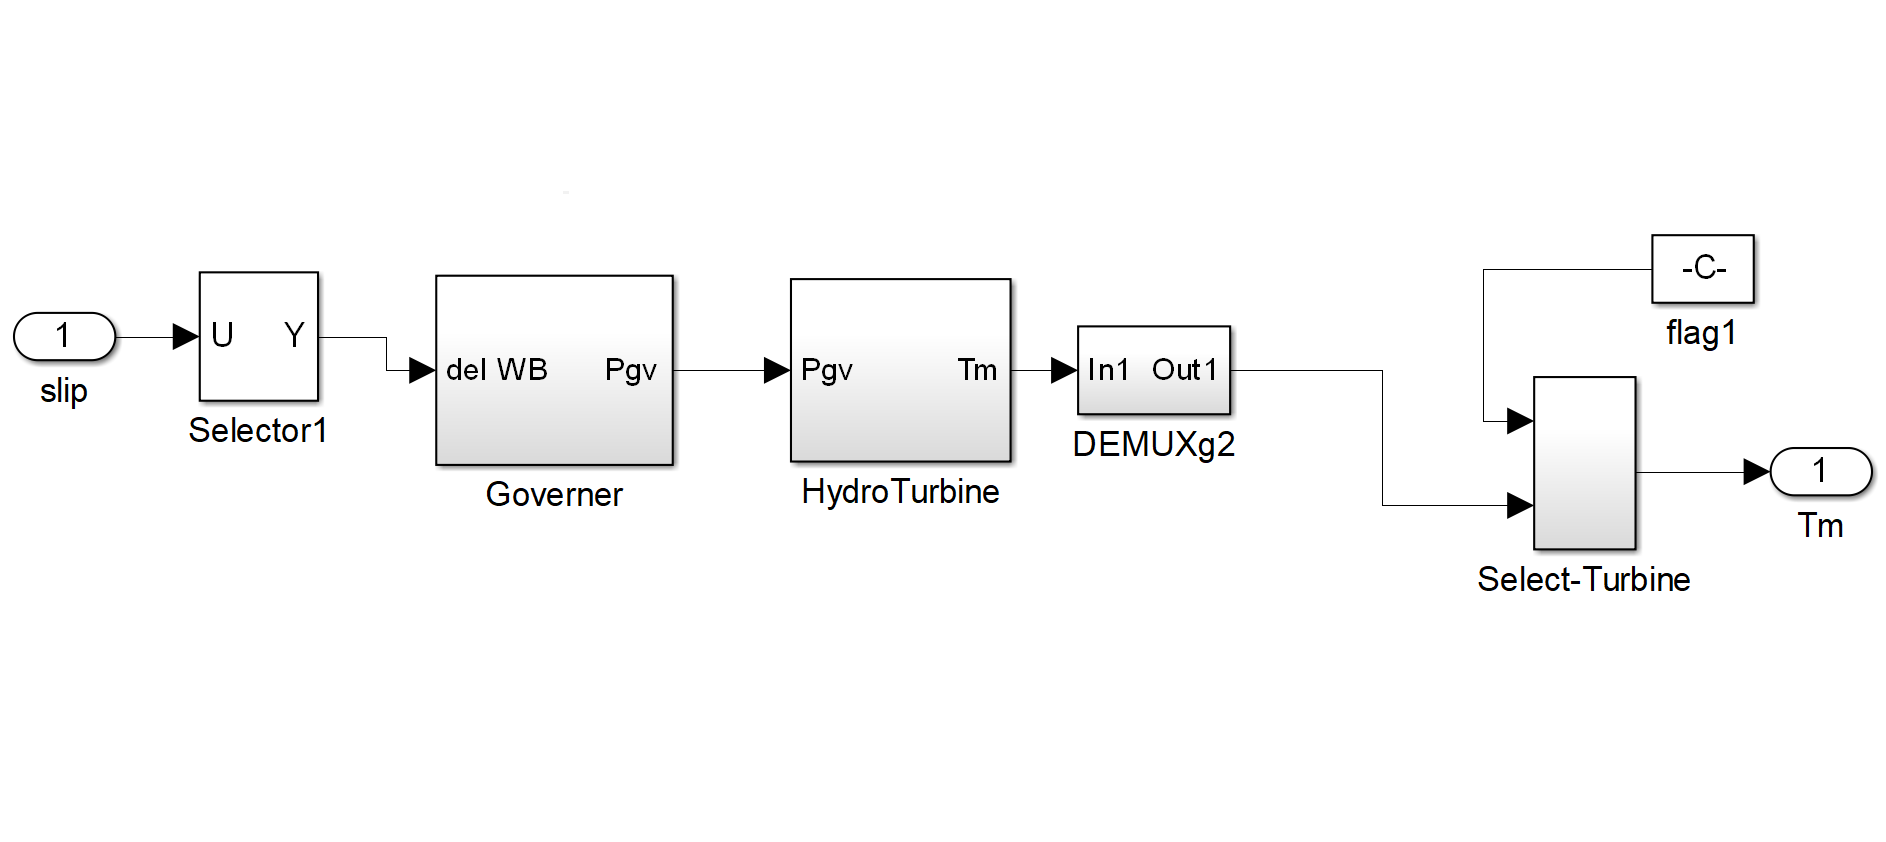
\includegraphics[scale=0.3]{Hydro governer speed turbine}
%		\caption{Hydro Turbine Speed governor}
%		\label{Hydro Turbine Speed governor}
%		\end{figure}
%		
%		\begin{figure}[H]
%		 \centering
%		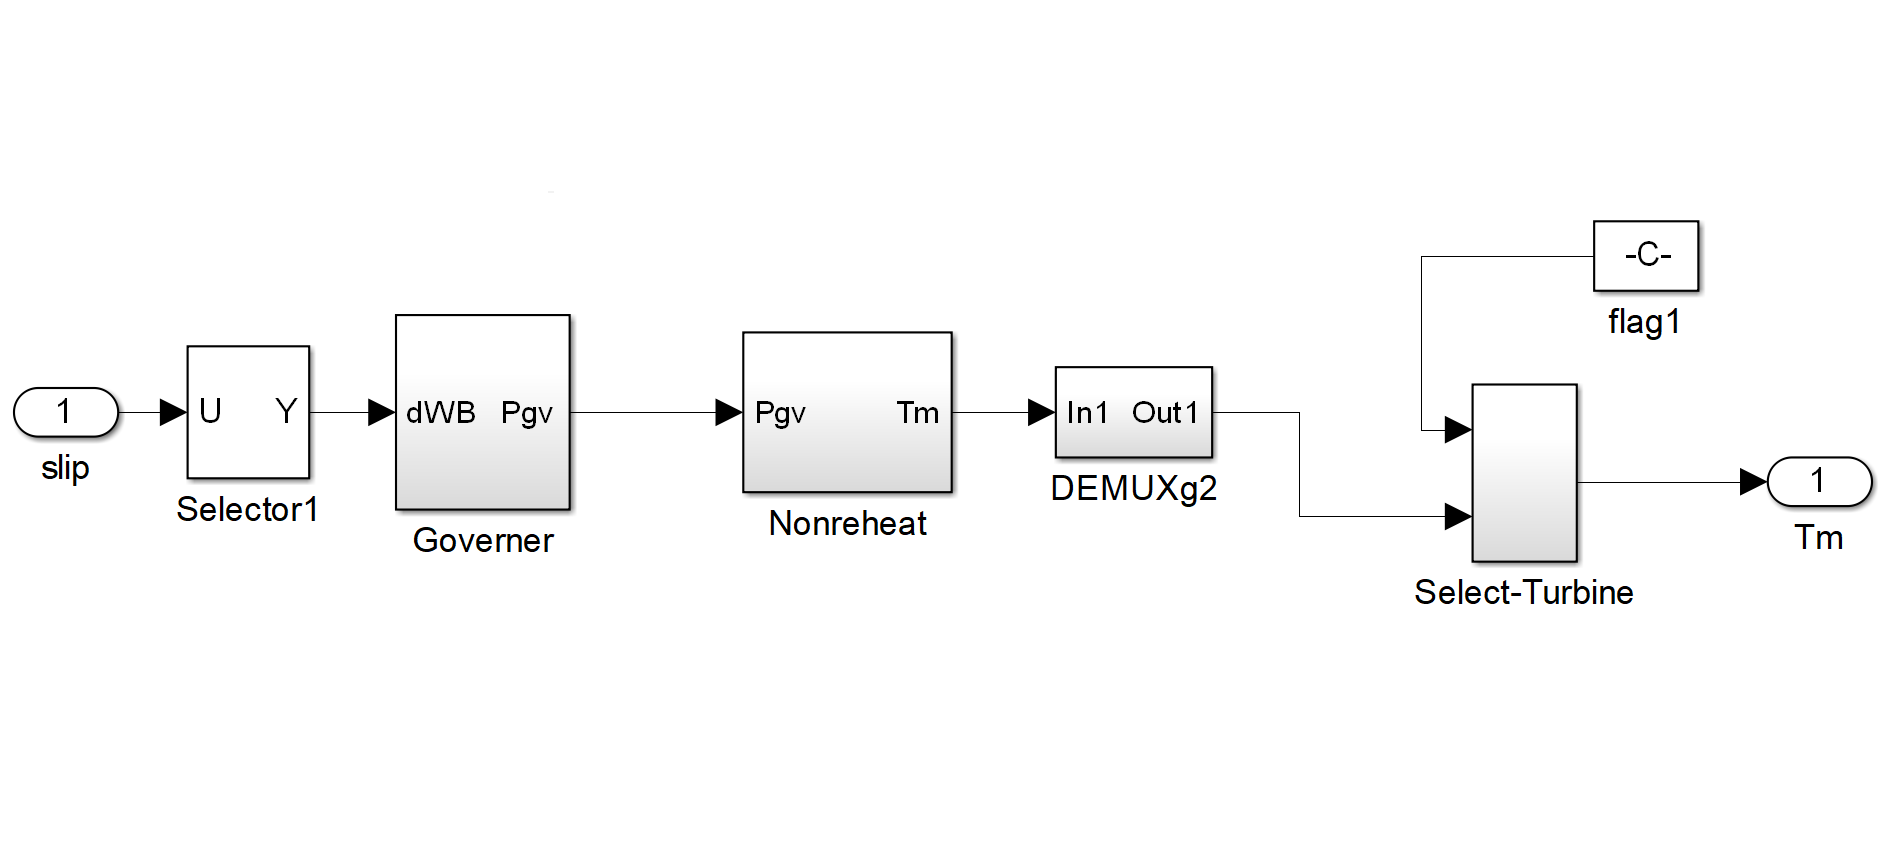
\includegraphics[scale=0.3]{Non Reheat Speed Turbine}
%		\caption{Non Reheat Turbine Speed Governor}
%		\label{Non Reheat Turbine Speed Governor}
%		\end{figure}
%		
%		\begin{figure}[H]
%		 \centering
%		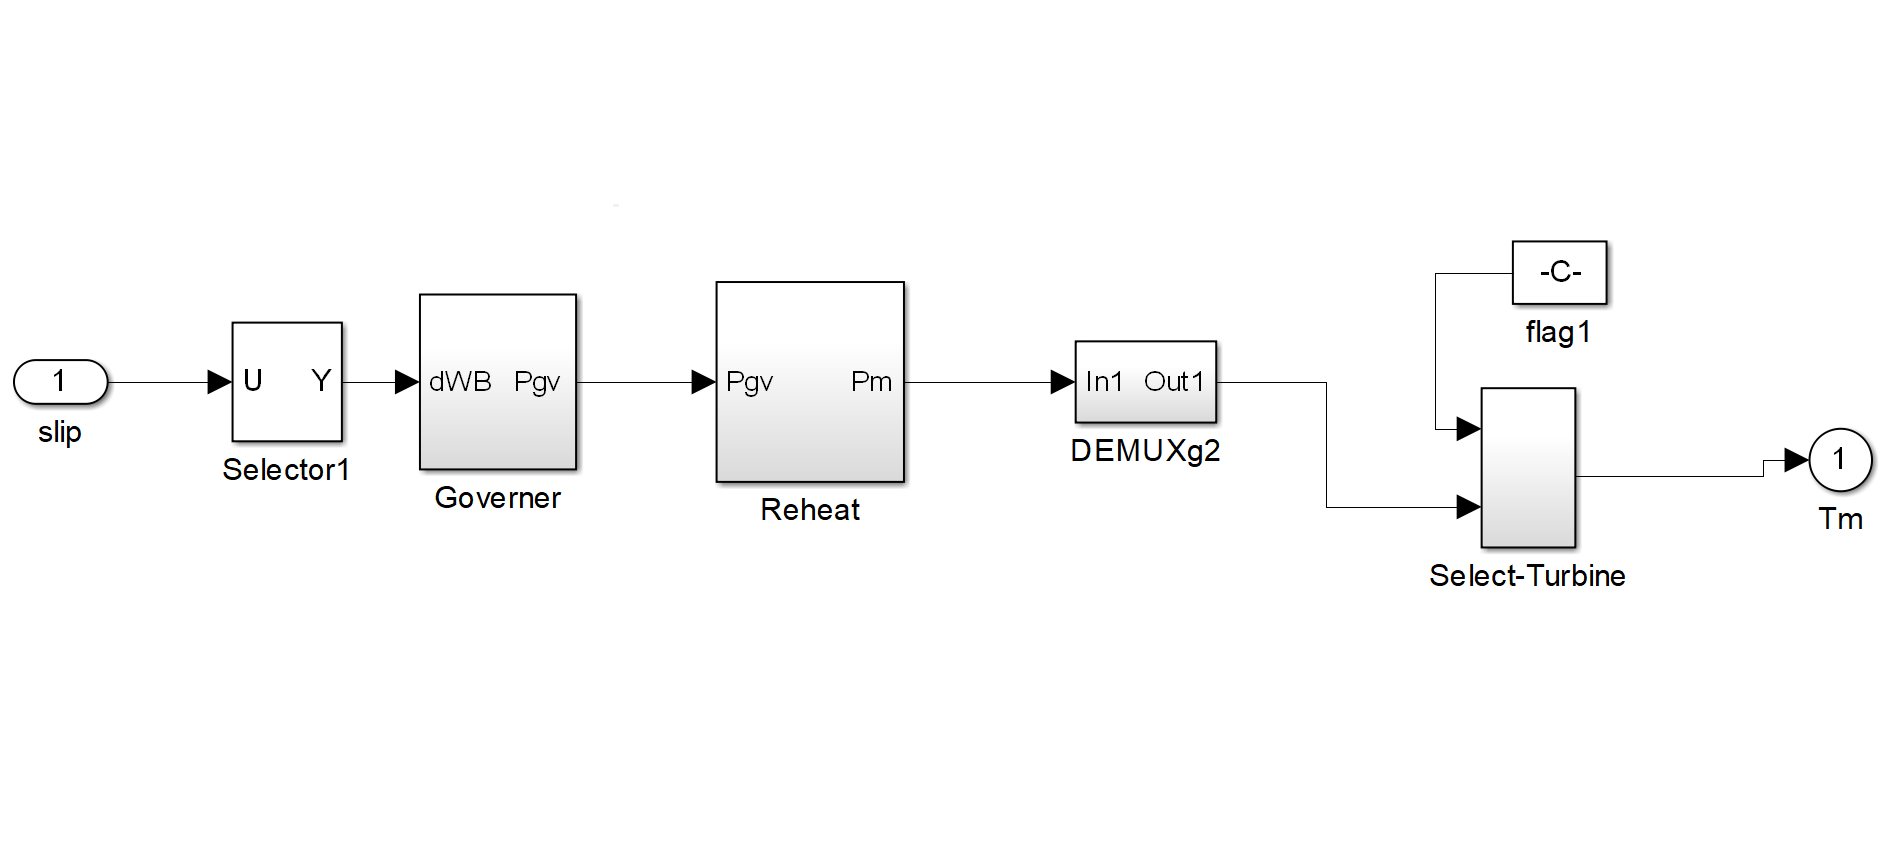
\includegraphics[scale=0.3]{Reheat Speed turbine Governor}
%		\caption{Reheat Turbine Speed Governor}
%		\label{Reheat Turbine Speed Governor}
%		\end{figure}
%	\end{itemize}
	
%% 3. Excitation System Model===================================================	
\item \textbf{\large Excitation System Model}: This is an excitation system created to do the work of an generator exciter, it takes input of Vg, Vs, IFD and Ig and with the help of different exciter system it  produces the Excitation voltage(EFD) and passes to the generator.
	
	\begin{figure}[H]
	 \centering
	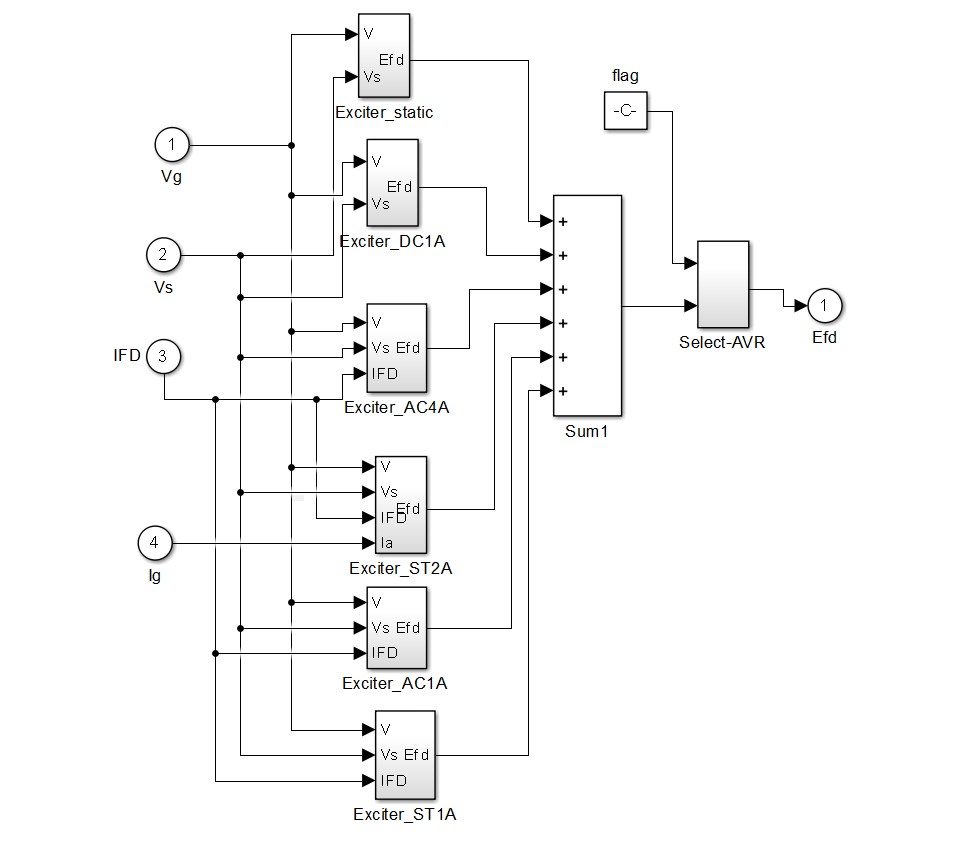
\includegraphics[scale=0.5]{Excitation Model}
	\caption{Excitation Model}
	\label{Excitation Model}
	\end{figure}
	
%	% Excitation System Sub Models-------------------------------------------------
%	\begin{itemize}
%	\item \textbf{\large Excitation System Sub Models}: Taking different inputs as stated in previous slide the different excitation sub part models are created to prepare whole Excitation System Model. The sum of these sub exciter models make a complete excitation system.
%		\begin{figure}[H]
%		 \centering
%		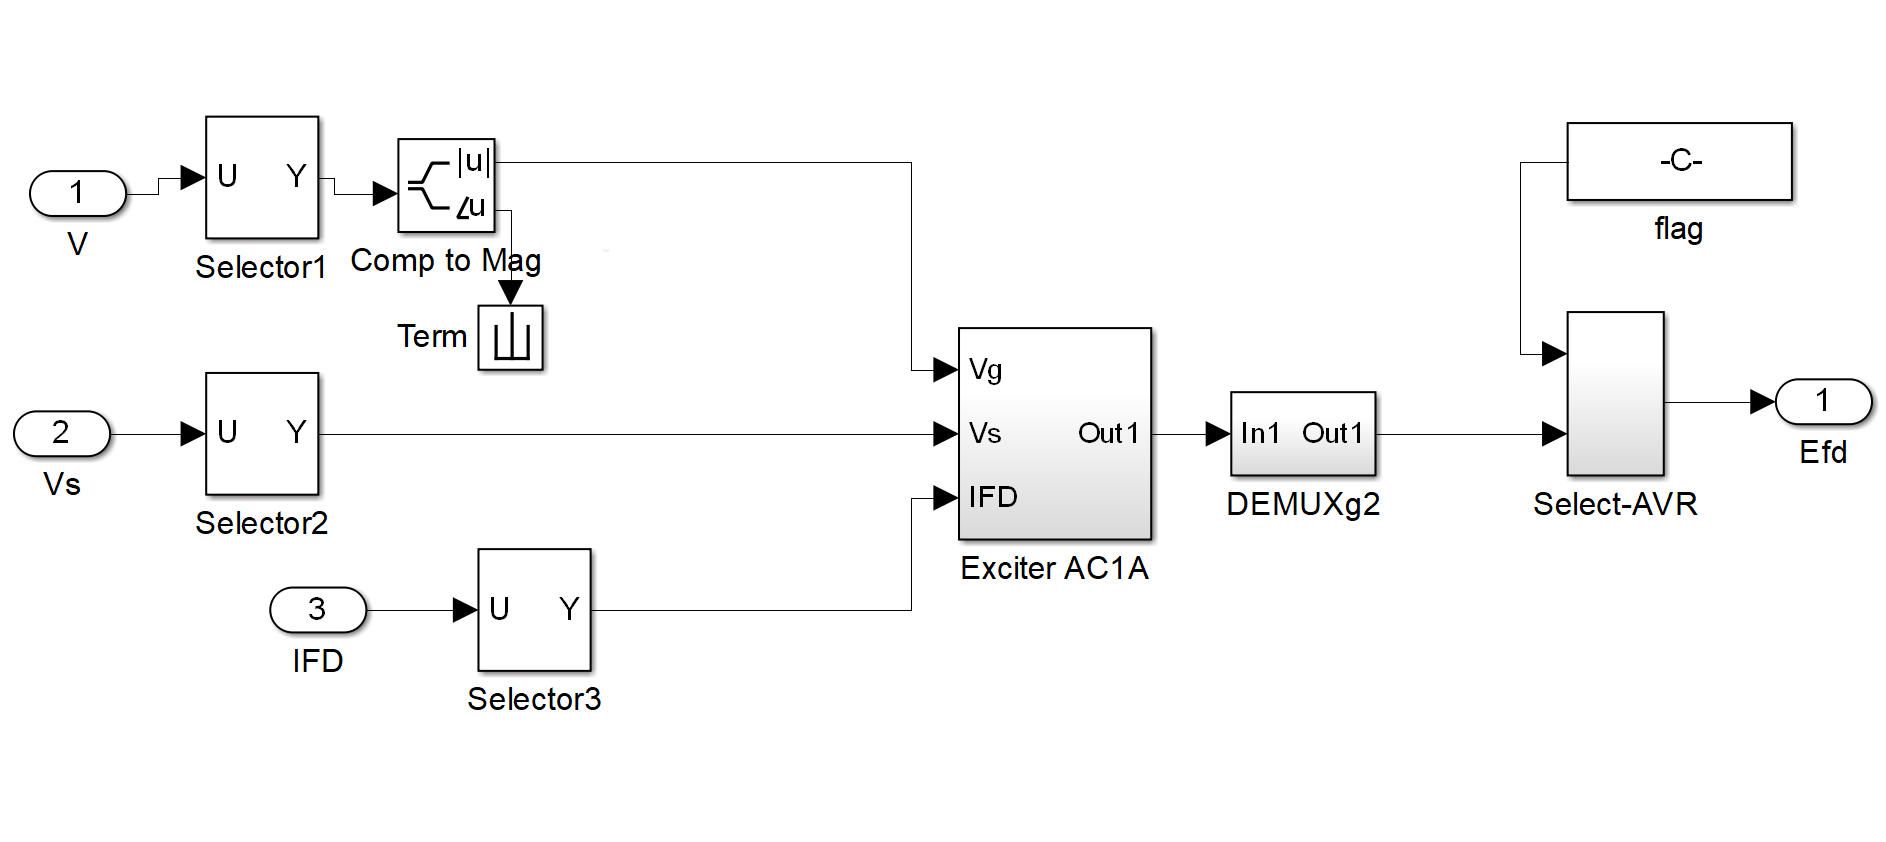
\includegraphics[scale=0.3]{Exciter AC1A}
%		\caption{Exciter AC1A}
%		\label{Exciter AC1A}
%		\end{figure}
%		
%		\begin{figure}[H]
%		 \centering
%		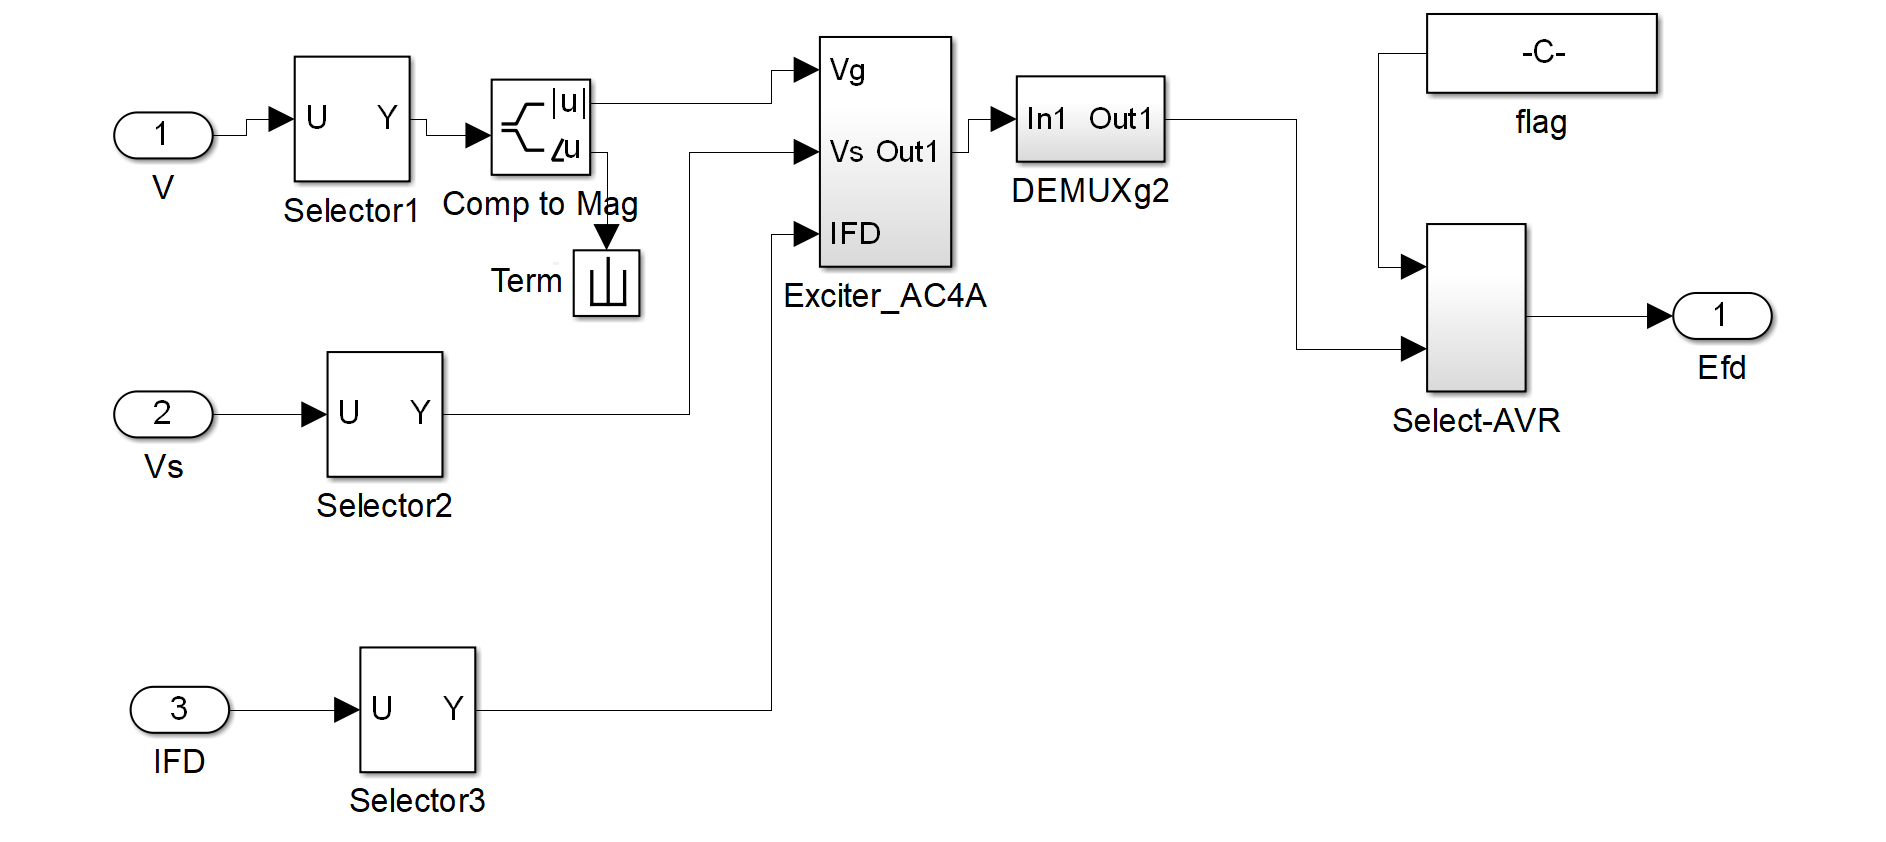
\includegraphics[scale=0.3]{Exciter AC4A}
%		\caption{Exciter AC4A}
%		\label{Exciter AC4A}
%		\end{figure}
%		
%		\begin{figure}[H]
%		 \centering
%		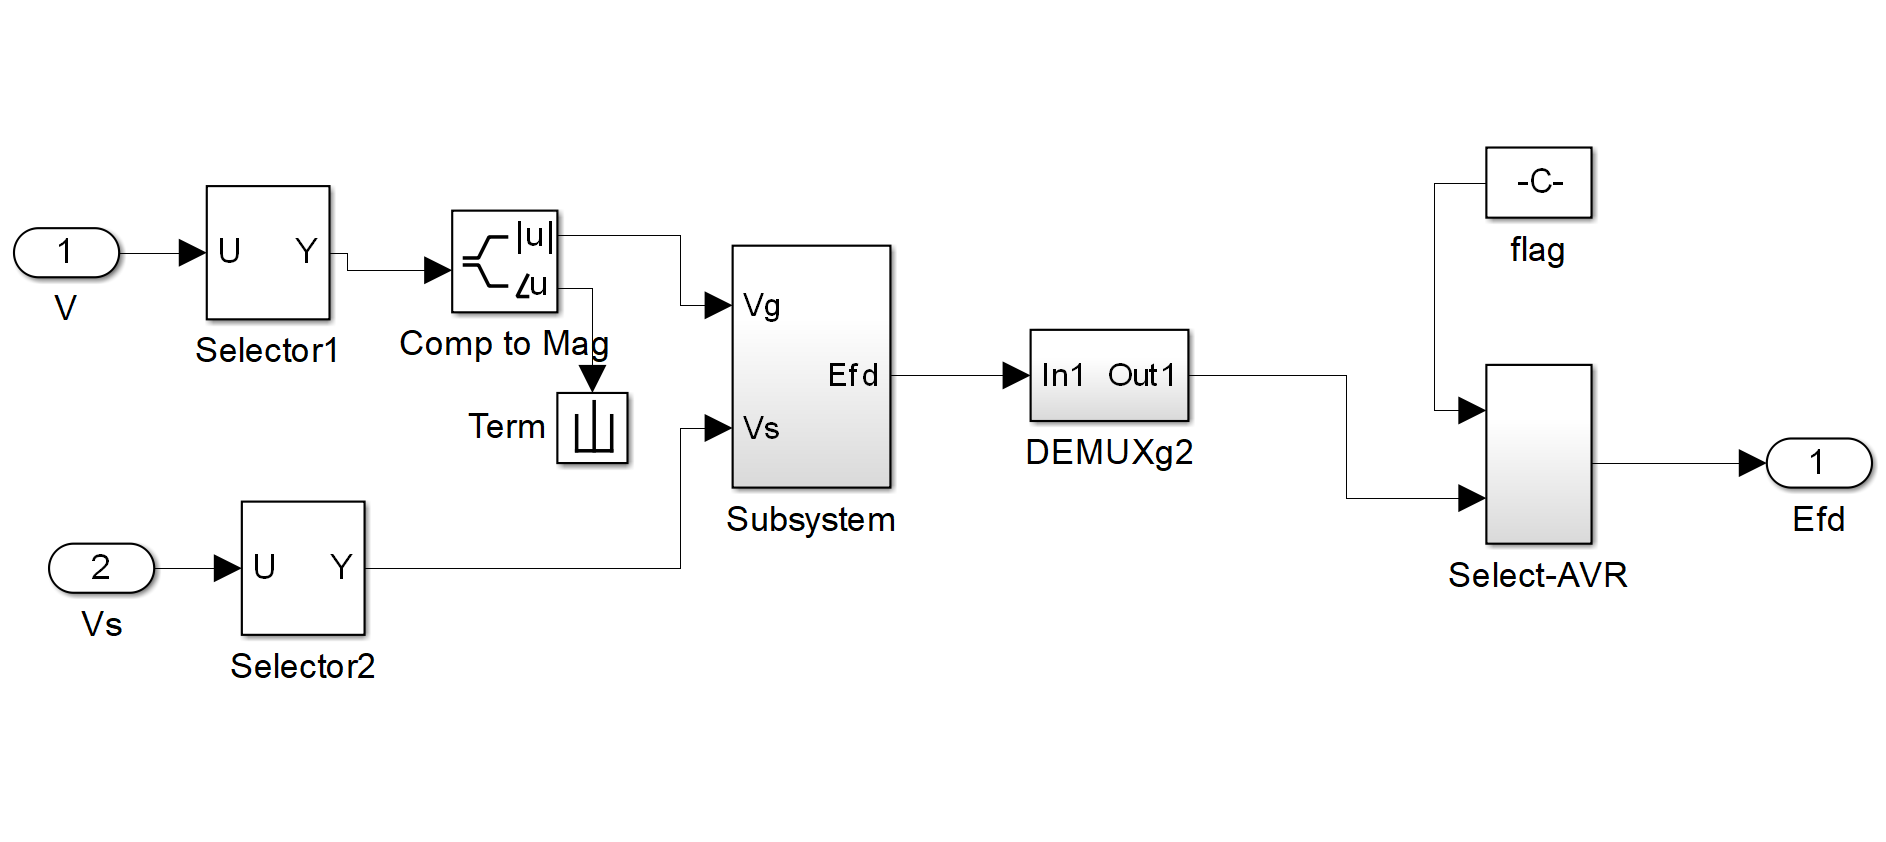
\includegraphics[scale=0.3]{Exciter DC1A}
%		\caption{Exciter DC1A}
%		\label{Exciter DC1A}
%		\end{figure}
%		
%		\begin{figure}[H]
%		 \centering
%		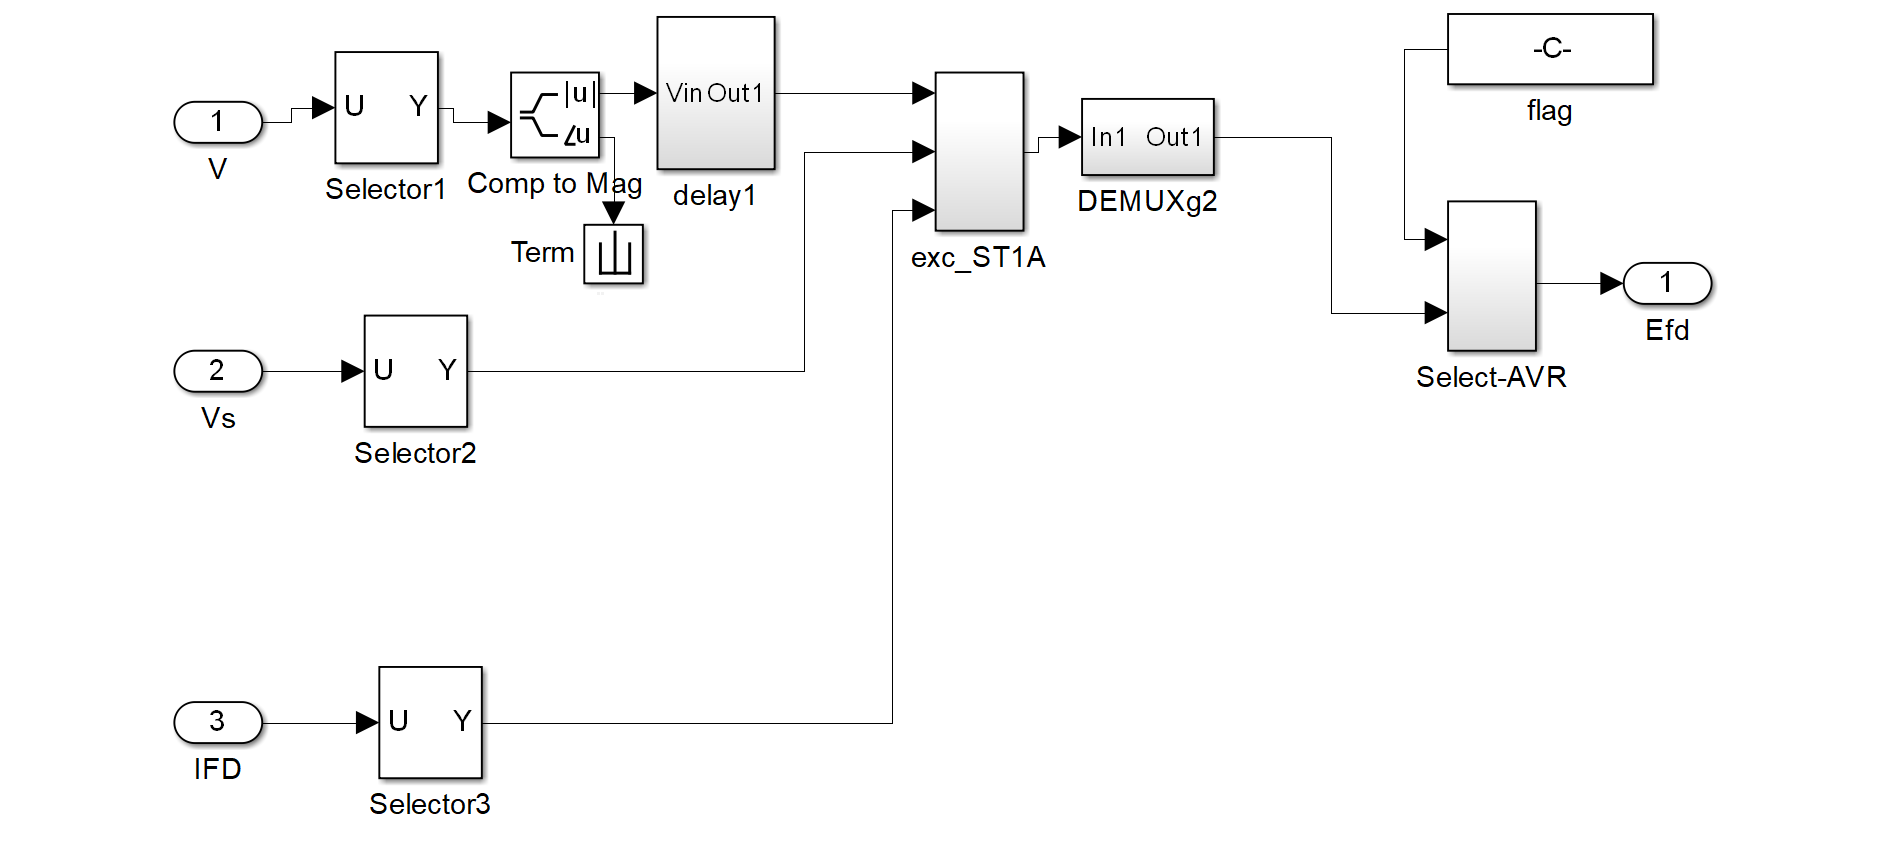
\includegraphics[scale=0.3]{Exciter ST1A}
%		\caption{Exciter ST1A}
%		\label{Exciter ST1A}
%		\end{figure}
%		
%		\begin{figure}[H]
%		 \centering
%		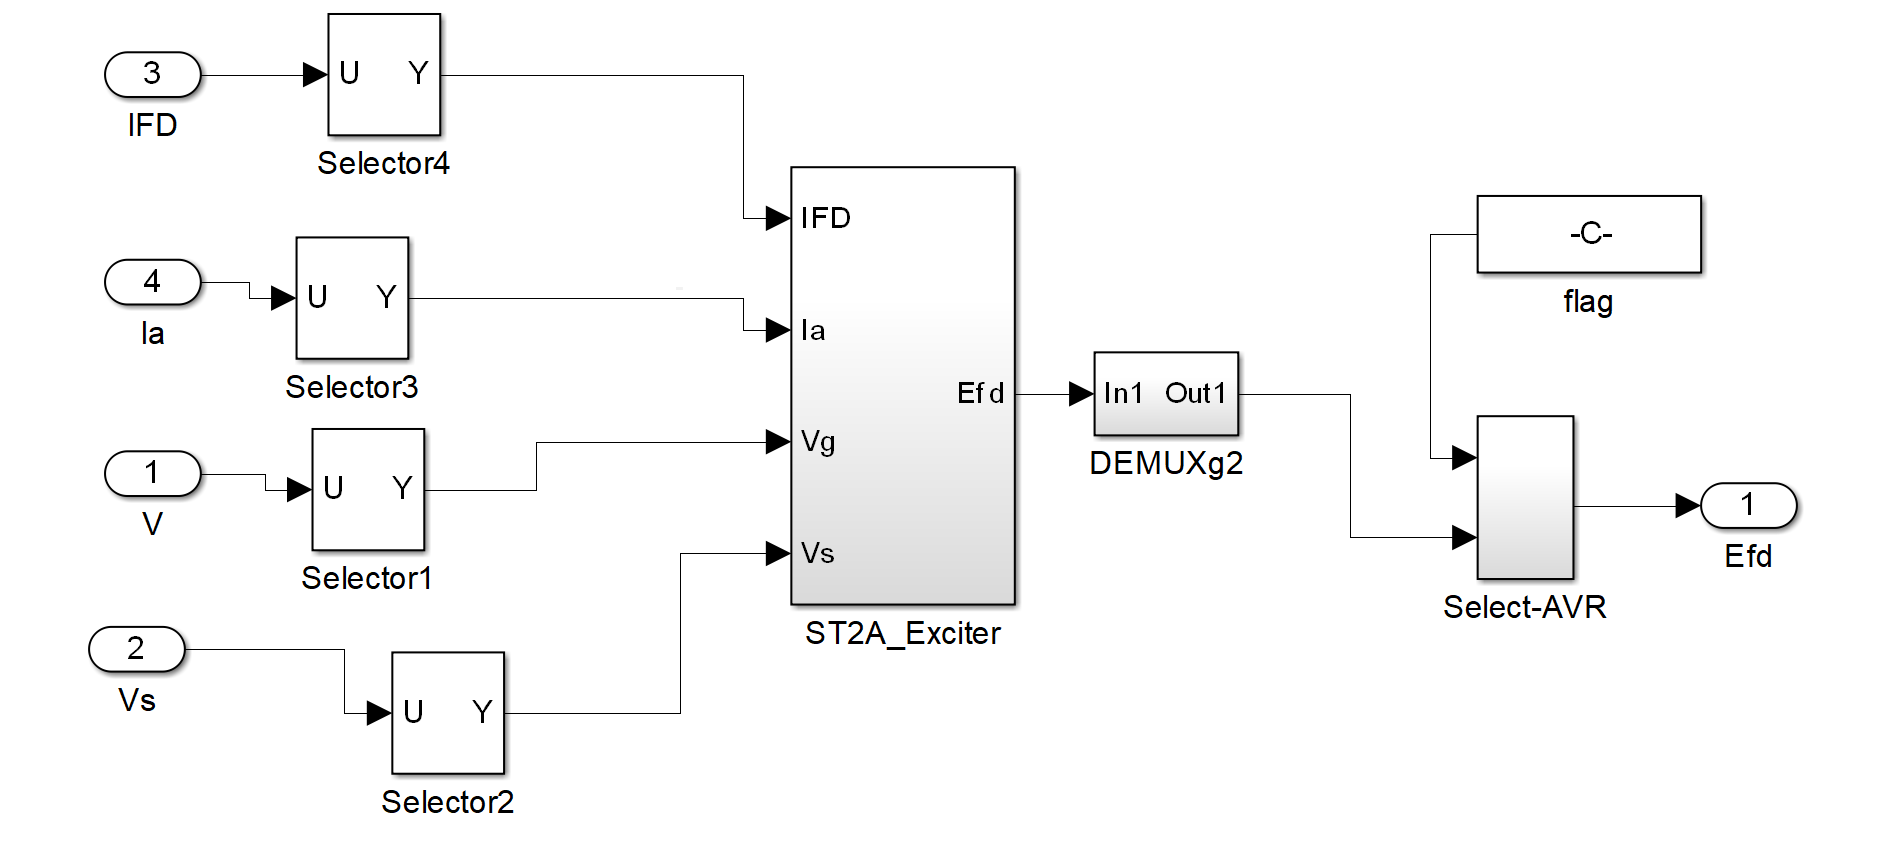
\includegraphics[scale=0.3]{Exciter ST4A}
%		\caption{Exciter ST4A}
%		\label{Exciter ST4A}
%		\end{figure}
%		
%		\begin{figure}[H]
%		 \centering
%		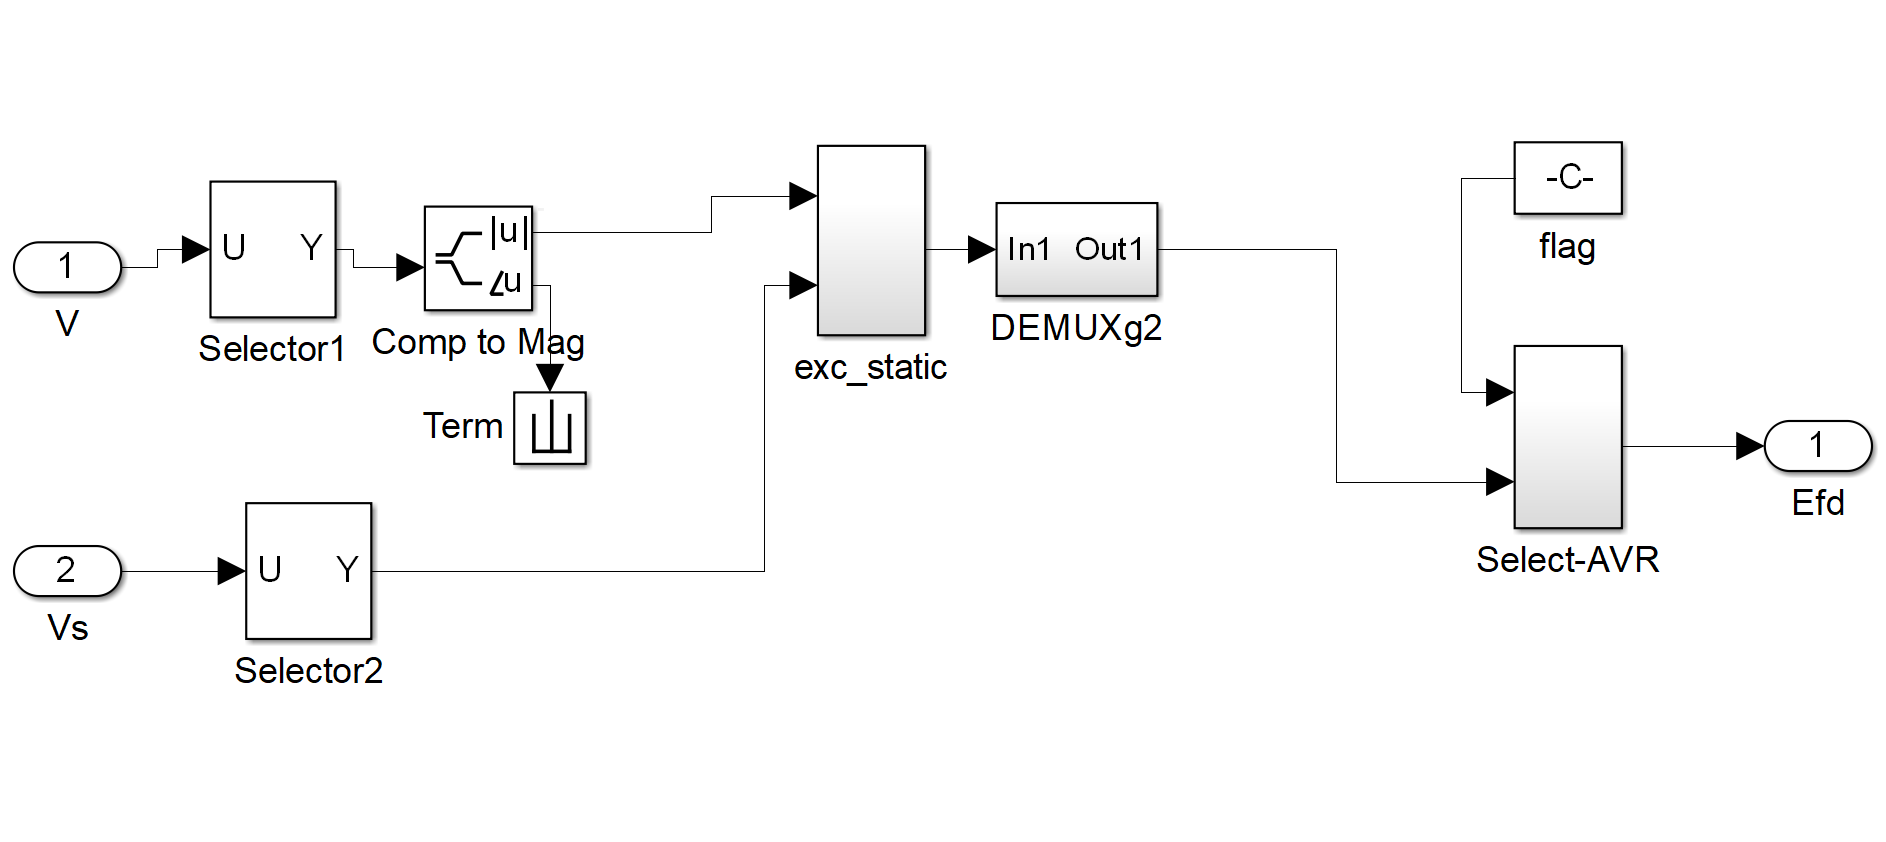
\includegraphics[scale=0.3]{Static Excitor System}
%		\caption{Static Exciter System}
%		\label{Static Exciter System}
%		\end{figure}
%				
%	\end{itemize}

%% 4. Static Loads Model===================================================	
\item \textbf{\large Static Load Model}: This simulation model is prepared to create a load system which uses active and reactive part to calculate the consumption by the load with the help of various mathematical formulas and gives the current output to the system to calculate power consumption.  
	
	\begin{figure}[H]
	 \centering
	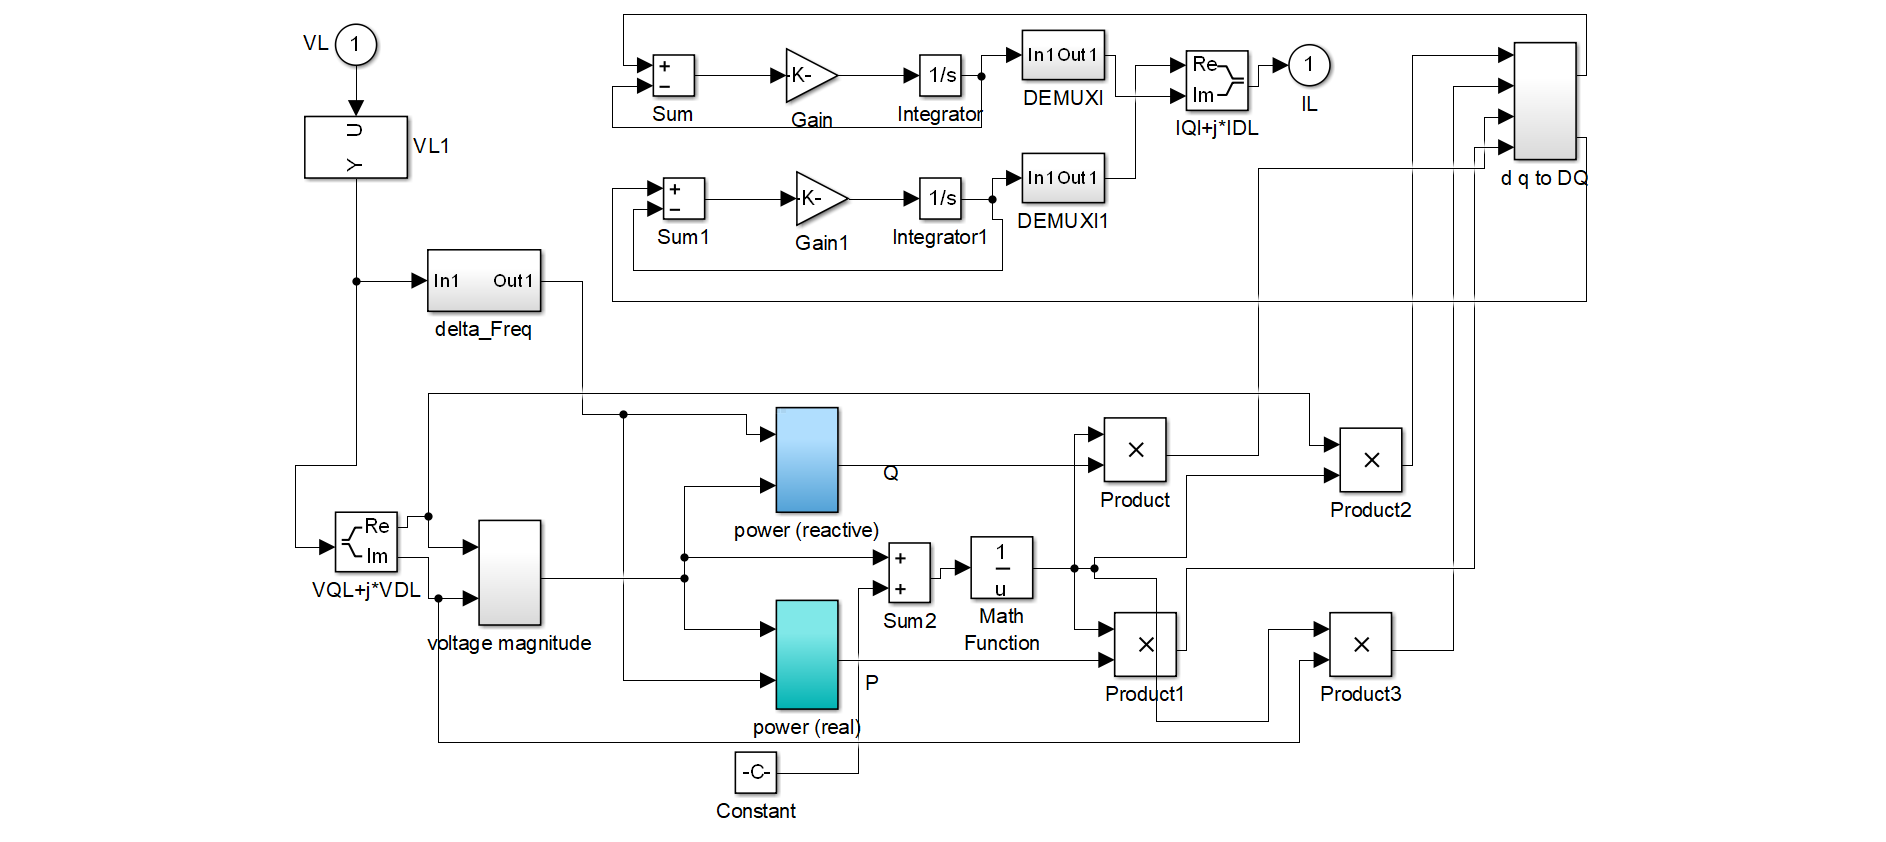
\includegraphics[scale=0.4]{Static Loads}
	\caption{Static Load Model}
	\label{Static Load Model}
	\end{figure}
	
%	% Static Load Sub Models-------------------------------------------------
%	\begin{itemize}
%	\item \textbf{\large Static Load Sub Models}: Static Load Model includes Voltage Magnitude, Real and Reactive Power models to calculate the consumption.
%		\begin{figure}[H]
%		 \centering
%		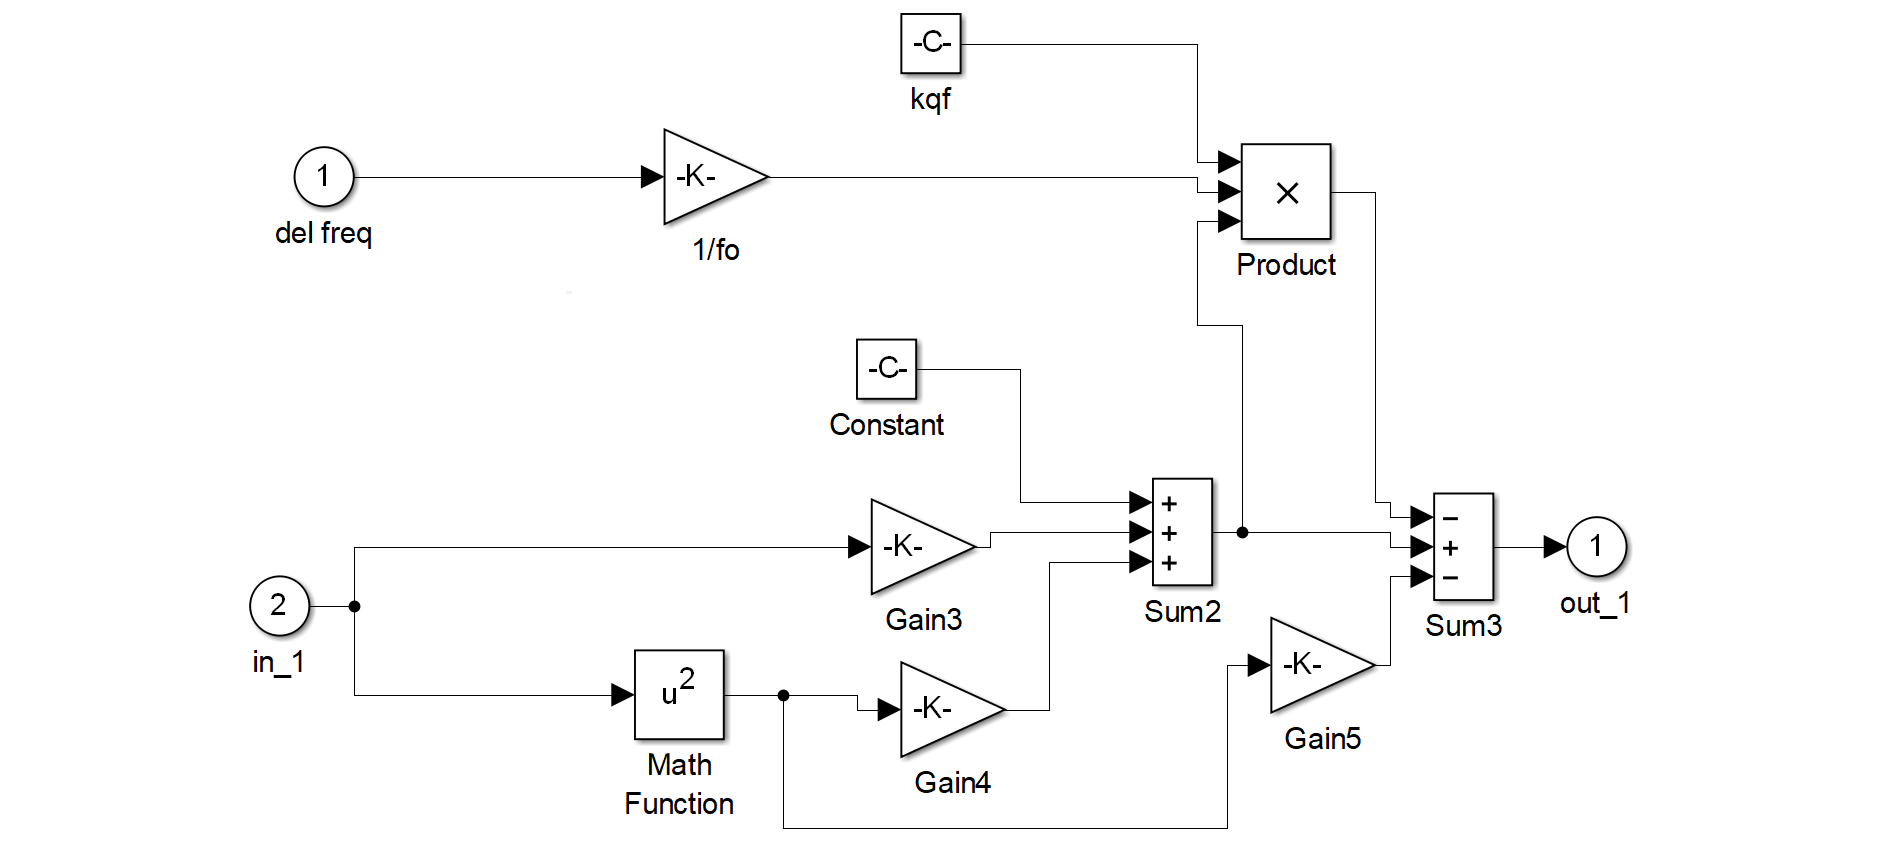
\includegraphics[scale=0.3]{Reactive Power}
%		\caption{Reactive Power Model}
%		\label{Reactive Power}
%		\end{figure}
%		
%		\begin{figure}[H]
%		 \centering
%		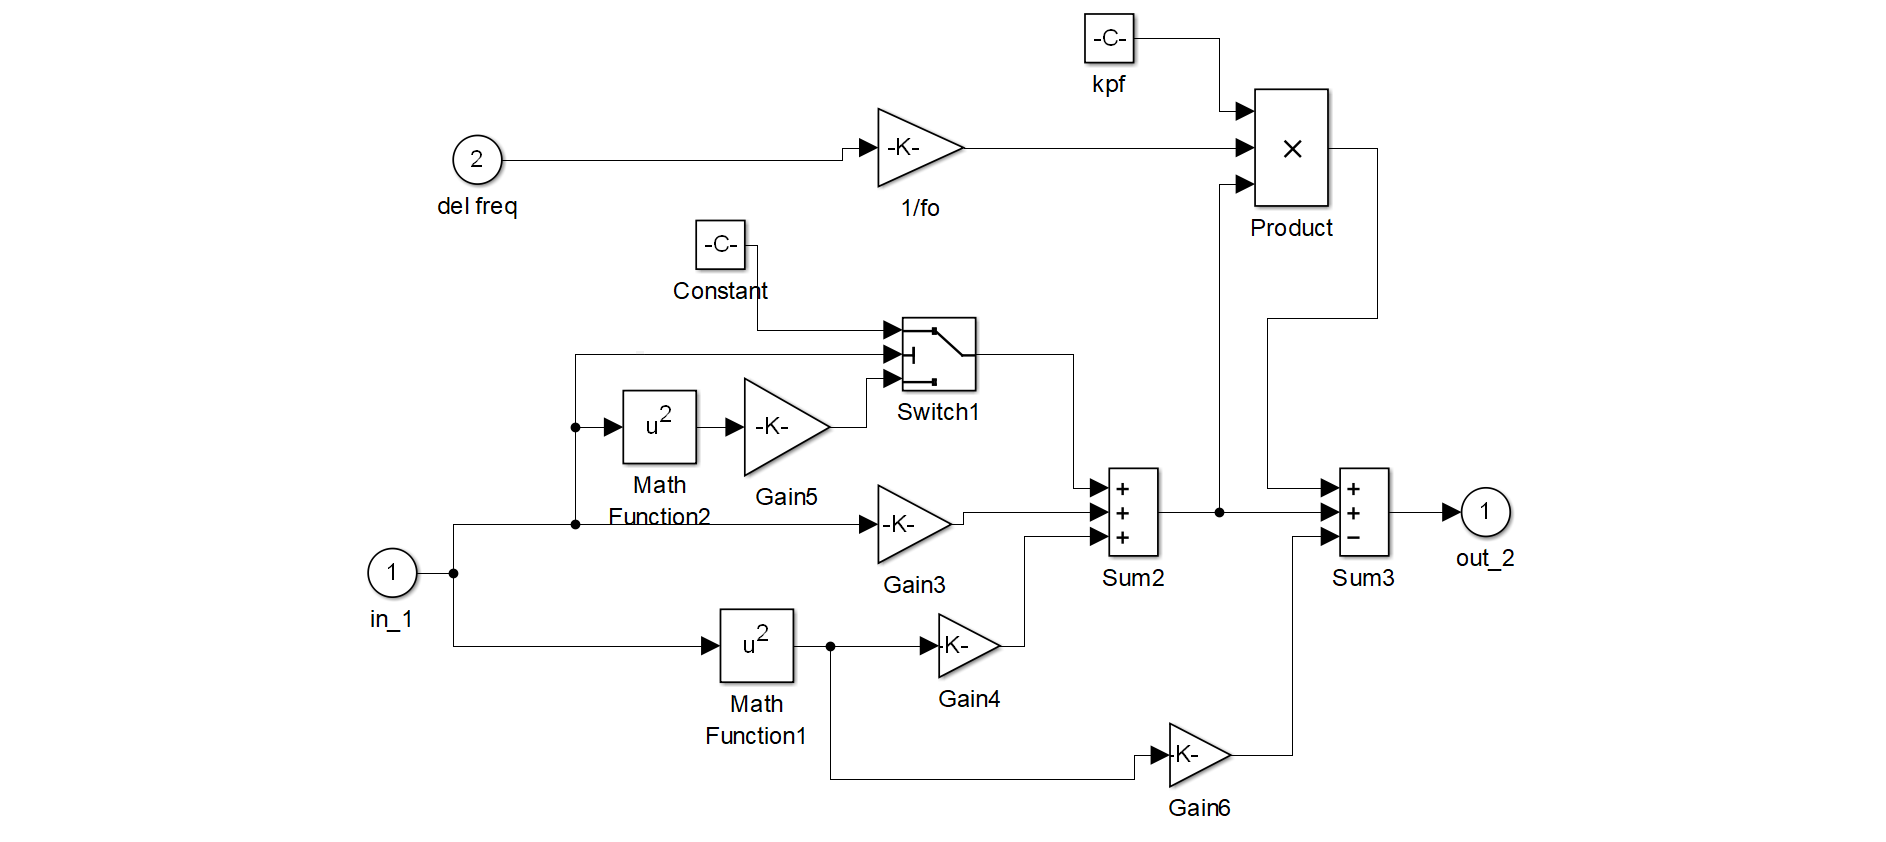
\includegraphics[scale=0.3]{Real Power}
%		\caption{Real Power Model}
%		\label{Real Power}
%		\end{figure}
%		
%		\begin{figure}[H]
%		 \centering
%		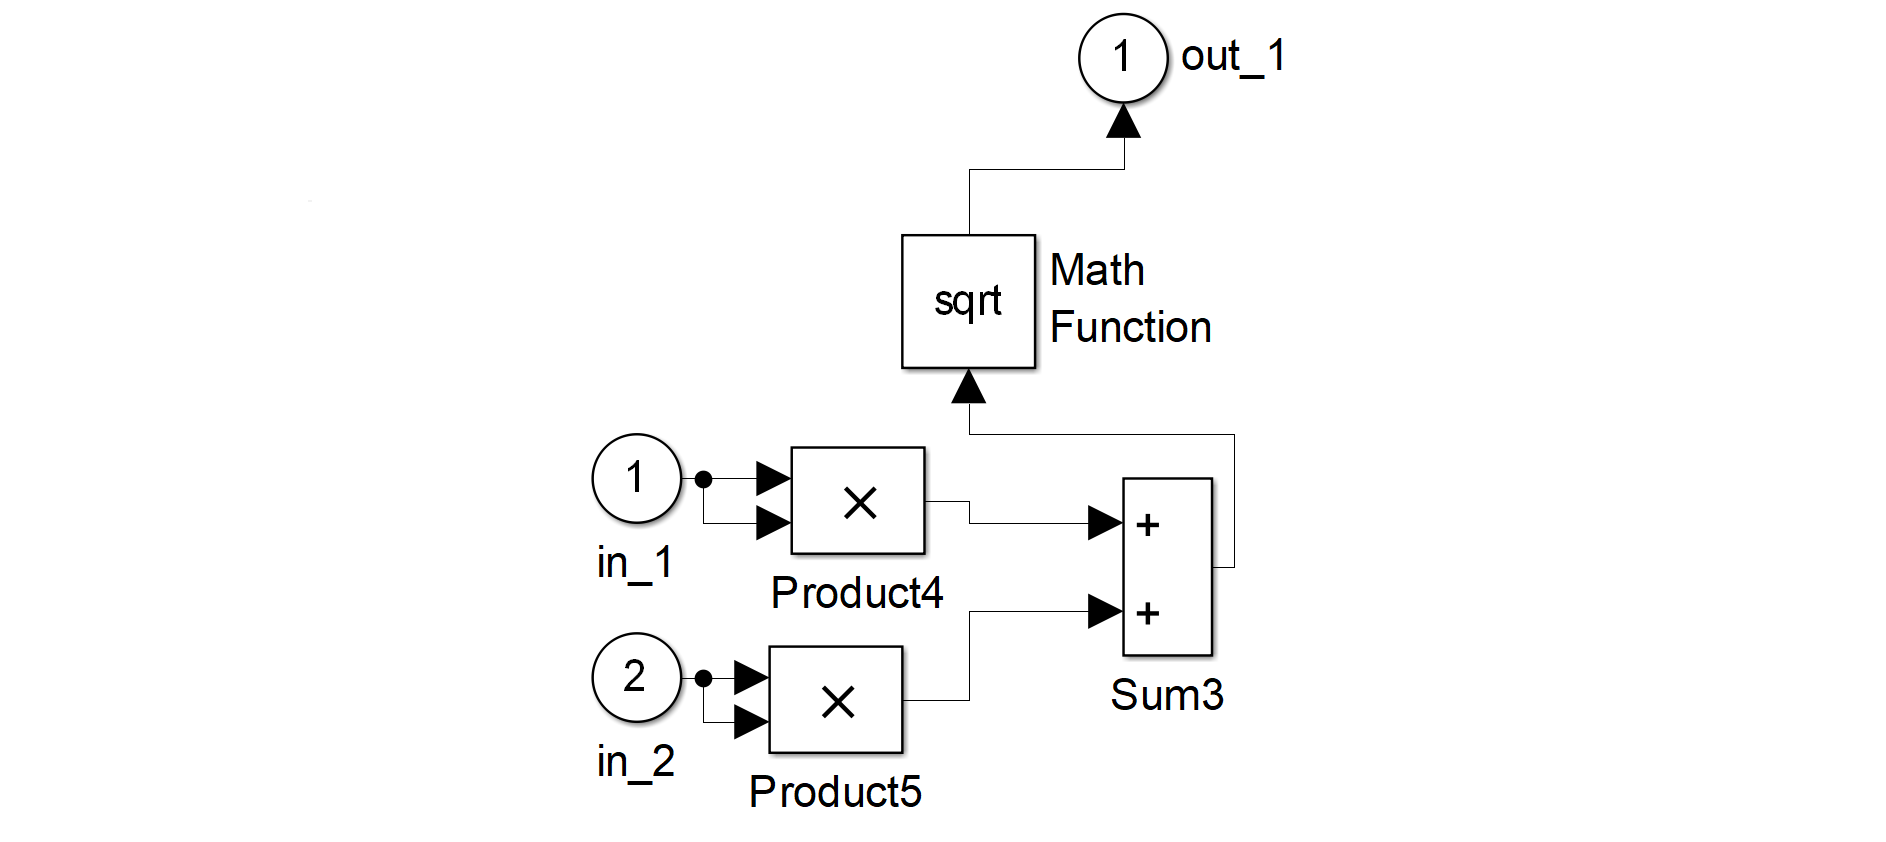
\includegraphics[scale=0.3]{Voltage Magnitude Calculation}
%		\caption{Voltage Magnitude Calculation}
%		\label{Voltage Magnitude Calculation}
%		\end{figure}
%		
%	\end{itemize}	

%% 5. PSS Model===================================================	
\item \textbf{\large Power System Stability Model}: It is created to give feedback to the excitation system according to the deviation of generator from the system parameters. It checks the generator slip and torque and bus voltage and by using four functions (Slip Signal, Power Input, Frequency Input and DelP\_Omega) it gives the feedback voltage.  
	
	\begin{figure}[H]
	 \centering
	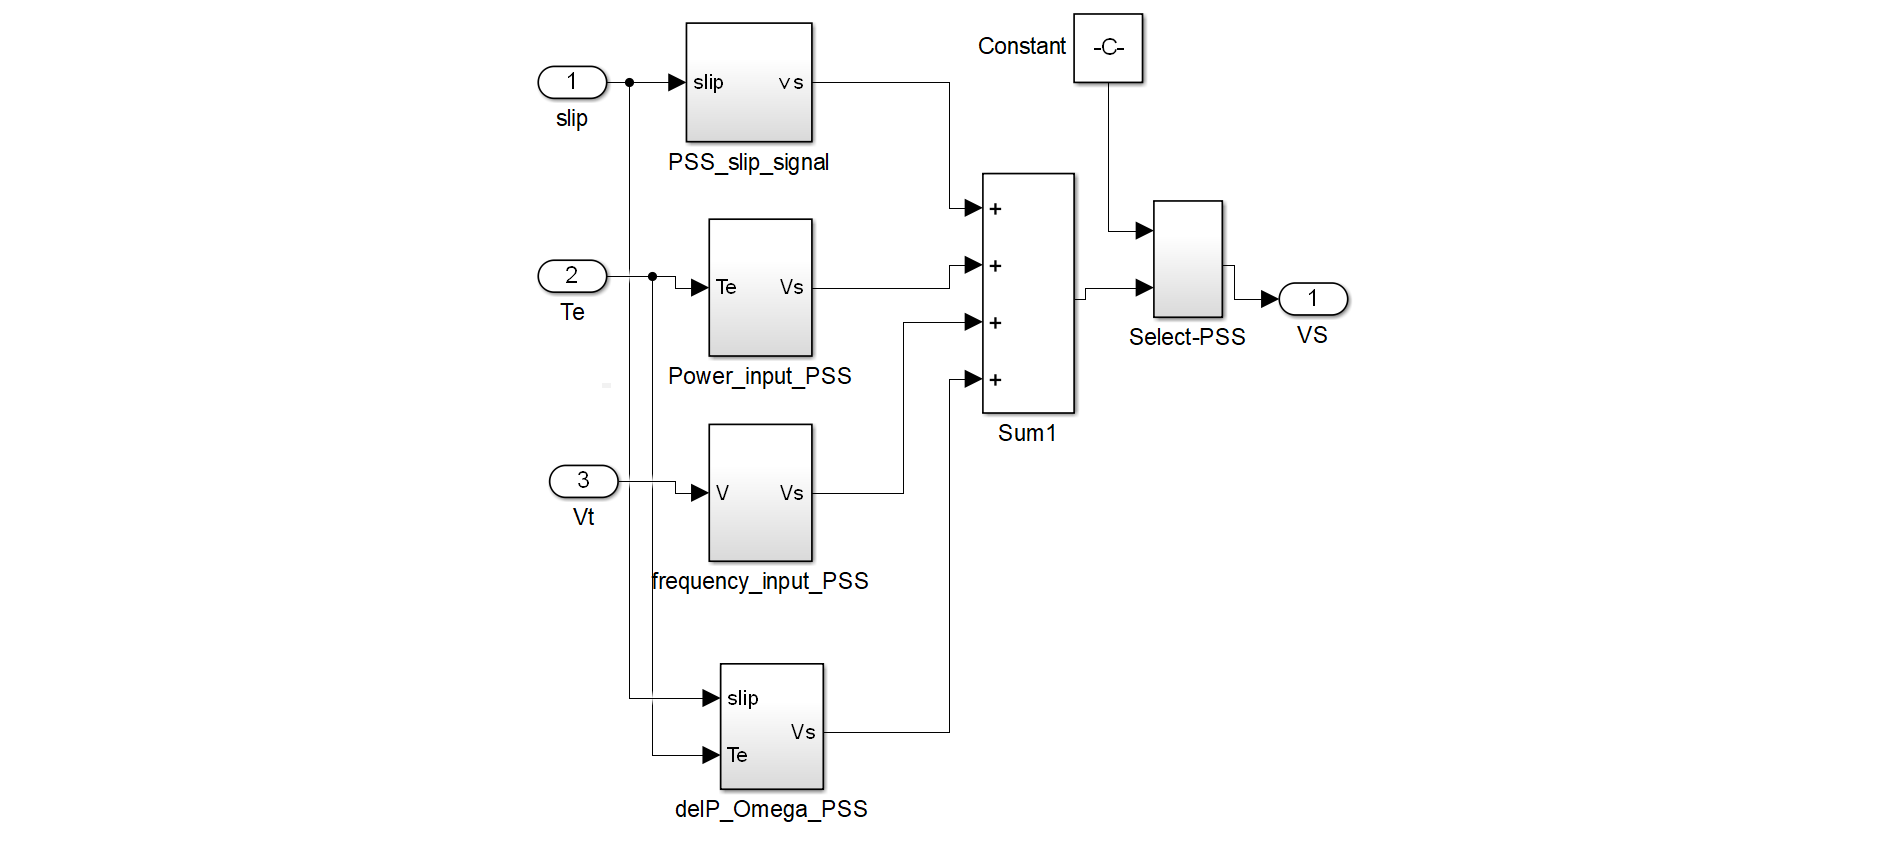
\includegraphics[scale=0.4]{PSS}
	\caption{Power System Stability Model}
	\label{Power System Stability Model}
	\end{figure}
	
%	% PSS Sub Models-------------------------------------------------
%	\begin{itemize}
%	\item \textbf{\large Power System Stability Sub Models}: Static Load Model includes Voltage Magnitude, Real and Reactive Power models to calculate the consumption.
%		\begin{figure}[H]
%		 \centering
%		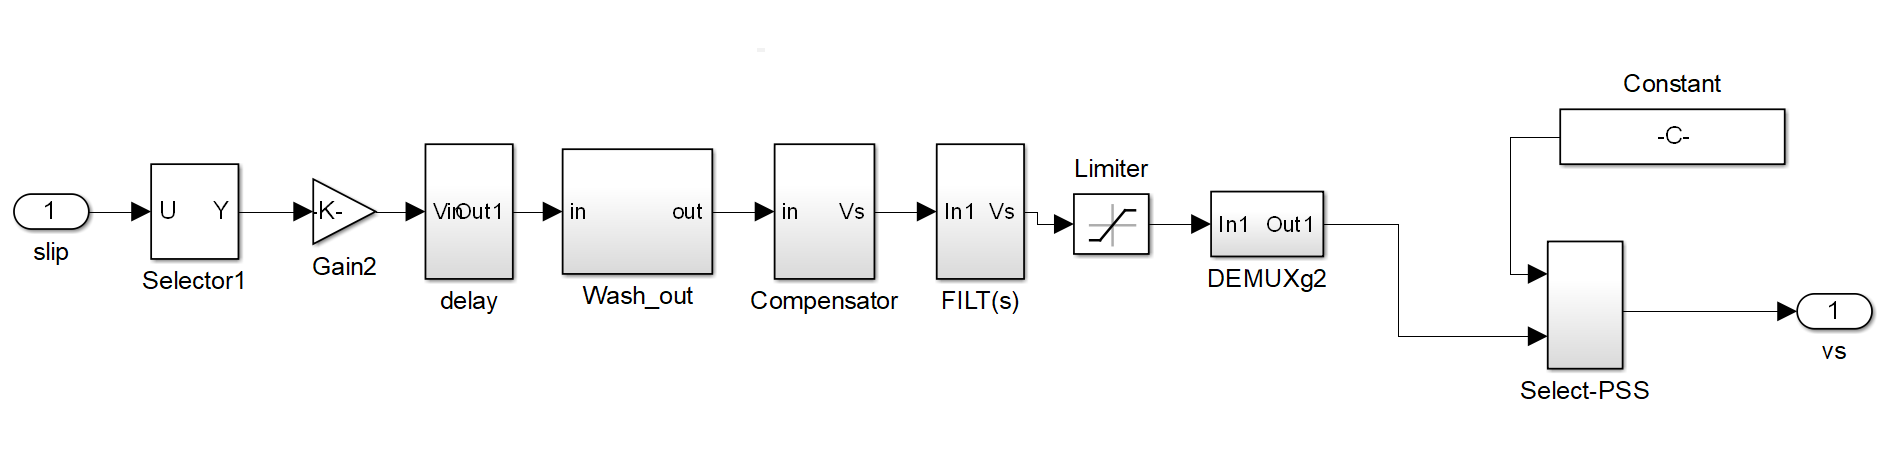
\includegraphics[scale=0.3]{Slip Signal PSS}
%		\caption{Slip Signal PSS}
%		\label{Slip Signal PSS}
%		\end{figure}
%		
%		\begin{figure}[H]
%		 \centering
%		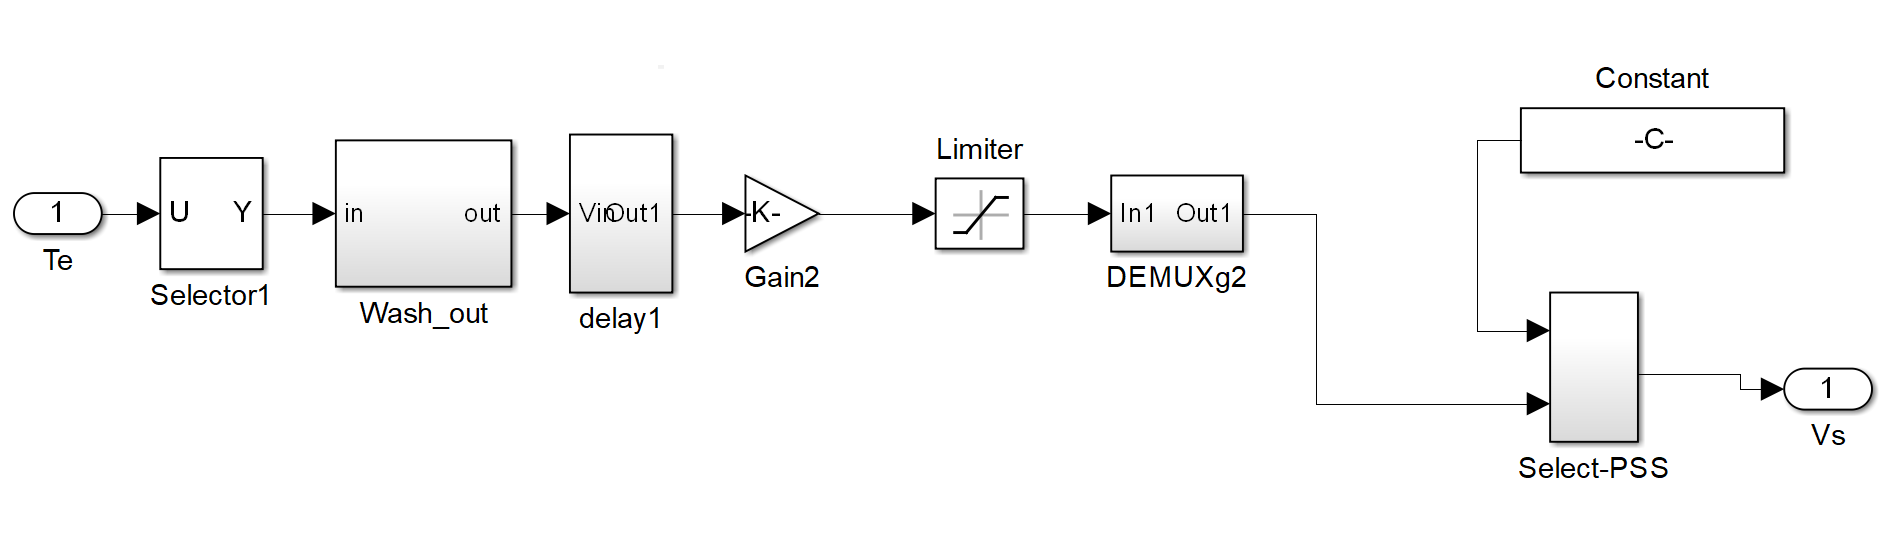
\includegraphics[scale=0.3]{Power Input PSS}
%		\caption{Power Input PSS}
%		\label{Power Input PSS}
%		\end{figure}
%		
%		\begin{figure}[H]
%		 \centering
%		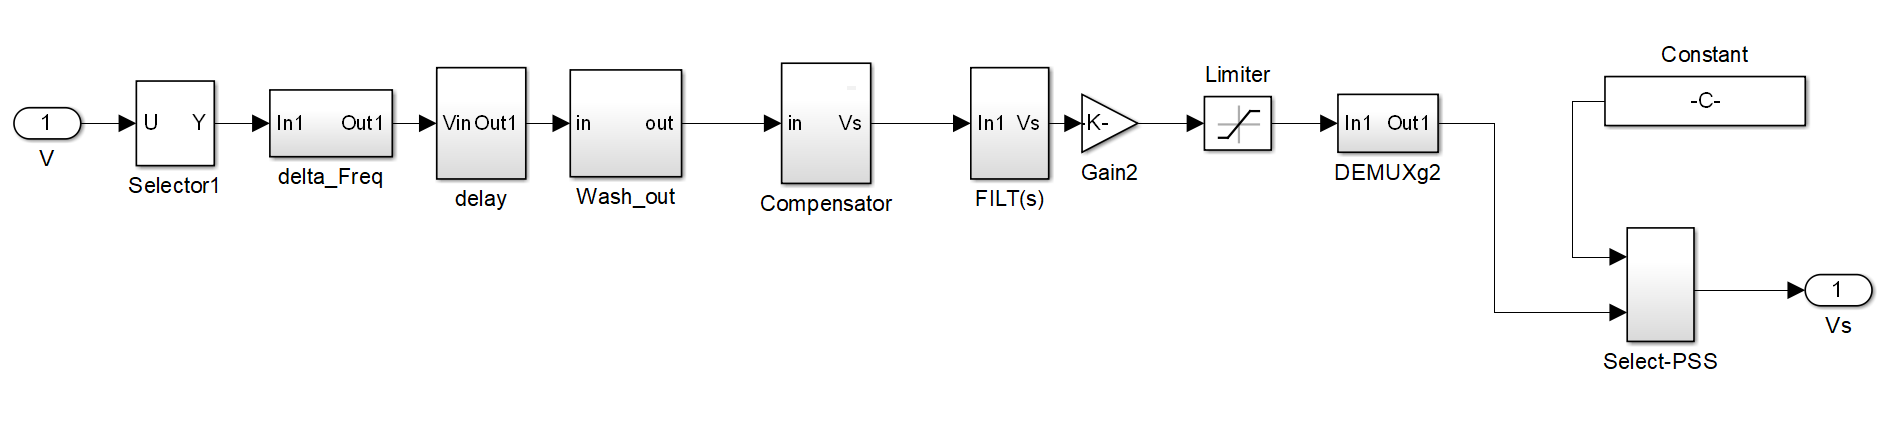
\includegraphics[scale=0.3]{Frequency Input PSS}
%		\caption{Frequency Input PSS}
%		\label{Frequency Input PSS}
%		\end{figure}
%		
%		\begin{figure}[H]
%		 \centering
%		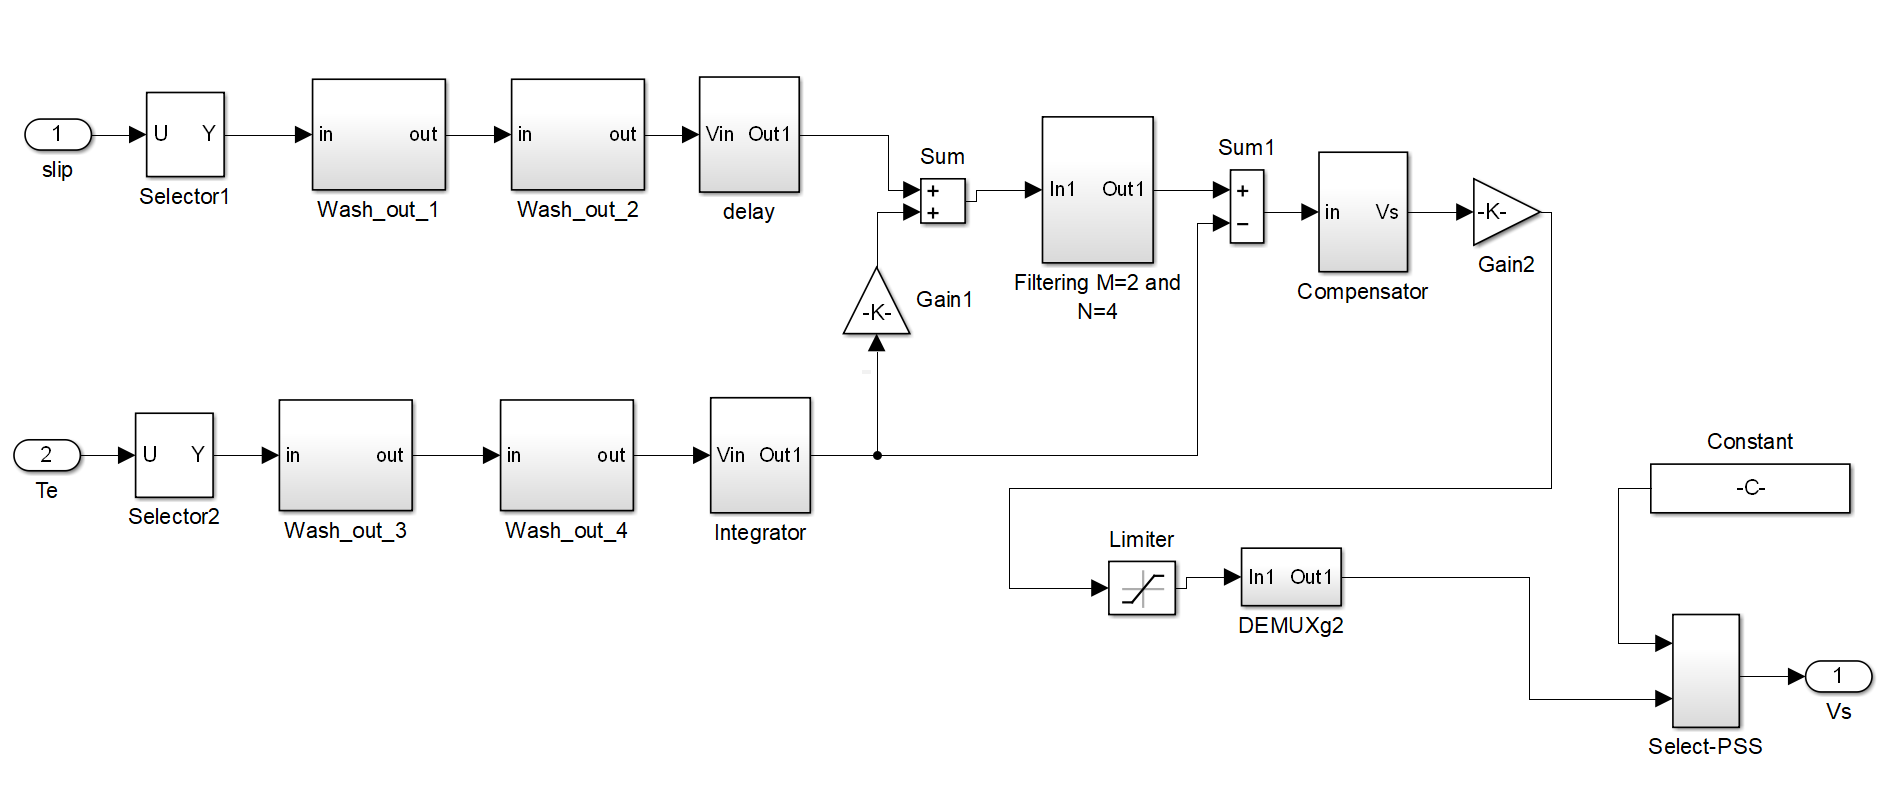
\includegraphics[scale=0.3]{delP Omega PSS}
%		\caption{DelP Omega PSS}
%		\label{delP Omega PSS}
%		\end{figure}
%	\end{itemize}	

%% 6. OUTPUT Model===================================================	
\item \textbf{\large System Parameters Output in Scope}: 8 System parameters (Generator Angle Deviation, Field EMF, Quadrature Axis Parameter, Direct Axis Parameter, Field Current, Mechanical Torque, Electrical Torque and System Voltage) are loaded to observe the result of transient stability of the system in graphical form.
	
	\begin{figure}[H]
	 \centering
	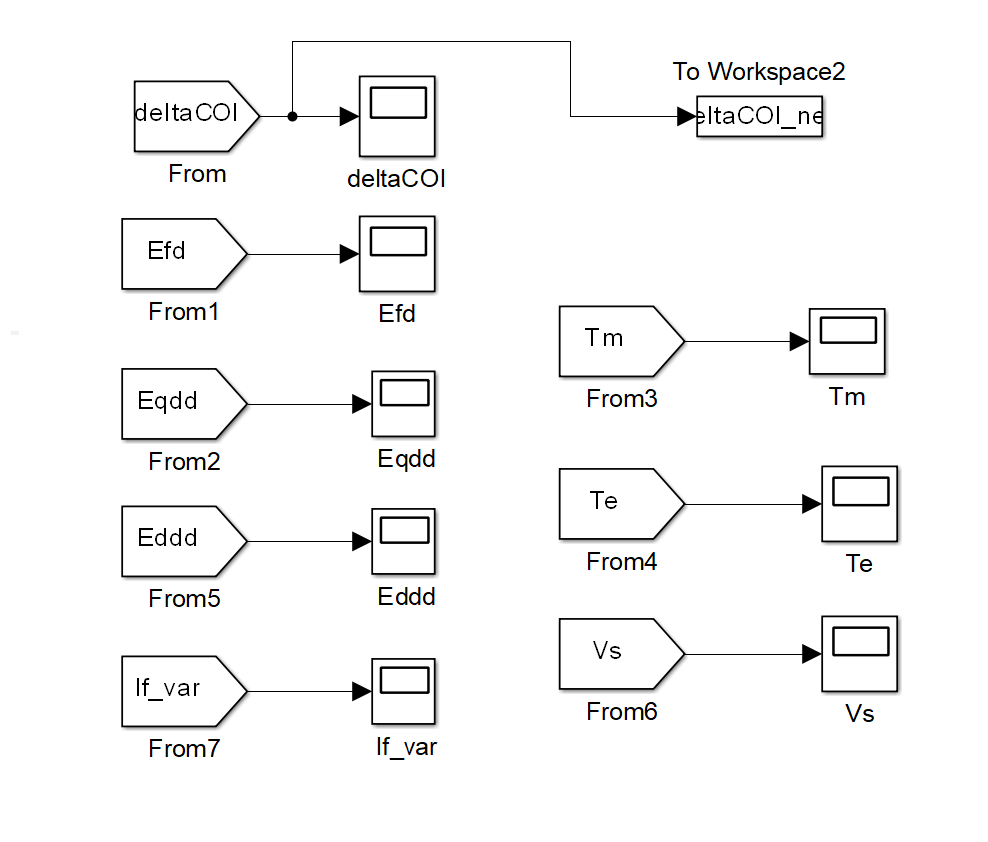
\includegraphics[scale=0.4]{output}
	\caption{System Parameters Output}
	\label{System Parameters Output}
	\end{figure}	
	
	
\end{enumerate}


\section{Computation of Indicators}
As Indicators are described before in section \ref{Catastrophic Indicators} briefly are used for analysing stability of the system after it experiences any type of fault. Generalized formulas of indicators (eqn. \ref{IS} to eqn. \ref{IL}) use system parameters shown in fig. \ref{System Parameters Output} to evaluate itself are used for evaluating the system stability. Analysis of Indicator has a main role of threshold values, which describe the system is stable or not. Selection of threshold vales depend upon the operator looking into the system parameters. Threshold vales are generally obtained from optimization or training Decision Trees. Threshold values are different for different type of contingencies. The proposed Catastrophic Indicators are summarized in Table \ref{Indicators}. These equations are solved and compared with threshold values to decide a system is table or not. The procedure of computation of Indicators is described in Algorithm \ref{Computation of Indicators}.

\begin{table}[!tb]

\renewcommand{\arraystretch}{2}
\caption{Proposed Catastrophic Indicators}
\label{Indicators}
%\begin{center}
\begin{tabular}{|P{0.2\linewidth} | P{0.8\linewidth}|}
\hline
 \textbf{NAME} & \textbf{INDICES}  \\ \hline
 Indicator based on Coherency & $Performance \; Index = max(max(\theta_i(t))-min(\theta_i(t)))$  \\ \hline
 Indicator based on Transient Energy Conversion & $Performance \; Index = max(max(|V_{ke}(t) - V_{pe}(t)|))$ \\  \hline 
 Indicator based on Dot Products (CSA) & $v(t) = \sum_{i=1}^{N_{area}} \omega_i(t)[\delta_i(t) - \delta_i(0^+)]$   \\ \hline
 Wide Area Severity Index (WASI) & $Fast WAST(T) = log(max_{t \; \in \; [0^+,T]}(max_i(PSD(V_i(t)))))$ \\  \hline 
 Inter-area Stability Prediction Index (ISPI) & $SPI = 1-(1-P\Delta V).(1-PV').(1-P\Delta d \delta gc).(1-Pd \delta gc') $ \\ \hline
\end{tabular}
%\end{center}
\end{table}

\begin{algorithm}[H]
\caption{Computation of Indicators}
\label{Computation of Indicators}
\begin{algorithmic}
\While {(a case in possibility dataset isn't handled)}
\begin{itemize}
    \item[--] Get the voltage and phase angle of all buses, as well as areawise and systemwise coherency measures, for the conceivable case.
\end{itemize}
\While {(an indicator isn't handled)}
\begin{itemize}
    \item[--] Figure the indicator values for the 20 ms (50 Hz)
time-stepped information of possibility case
    \item[--] Examine the strength condition in terms of its maximum value and label the instance as stable or unstable.
    \item[--] Update the case with the Indicator name and the condition of its soundness.
\end{itemize}
\EndWhile
\State \textbf{end while}
\EndWhile
\State \textbf{end while}
\end{algorithmic}
\end{algorithm} % Descrition of Software
\chapter{Results and Discussion}
\section{Stability Analysis in 10 Bus 4 Generator System}
\label{contingency1}
A realistic 4-machine 10-bust network design is presented to demonstrate the working of the suggested Catastrophic indicator. The organization's graphical chart can be found in Fig. \ref{fig:Line Diagram}. Prepare a model dataset as follows:
\begin{enumerate}
\item A consistent state working point is designated a base powerflow.
\item At 0.5 s, a three-stage cutoff is implemented at bus 9. (Tfault).
\item By opening the line between bus 9 and bus 10, the deficiency is resolved in 0.1 second (Tclear) (line possibility).

\end{enumerate}

\begin{figure}[H]
  \centering
  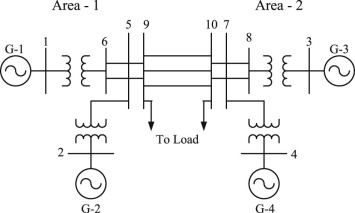
\includegraphics[width=0.6\linewidth]{LD}
  \caption{Line Diagram of two area 4 Machine 10 Bus Power System}
  \label{fig:Line Diagram}
\end{figure}

Initially the assumed fault is provided to the each bus system and the system parameters are observed. The further steps as described in Algorithm \ref{Computation of Indicators} are carried out using set of codes. So, assuming the fault initiated at 0.5 sec, for different fault clearing time, the faulted bus is provided for observing the transient stability result.

\subsection{Results for Indicator based on Coherency}
\label{Ind1}
\begin{figure}[H]
\centering
\begin{subfigure}{.5\textwidth}
  \centering
  \includegraphics[width=\linewidth]{Co No fault}
  \caption{Speed Deviation Vs. Time for No Fault}
  \label{fig:I1sub1}
\end{subfigure}%
\begin{subfigure}{.5\textwidth}
  \centering
  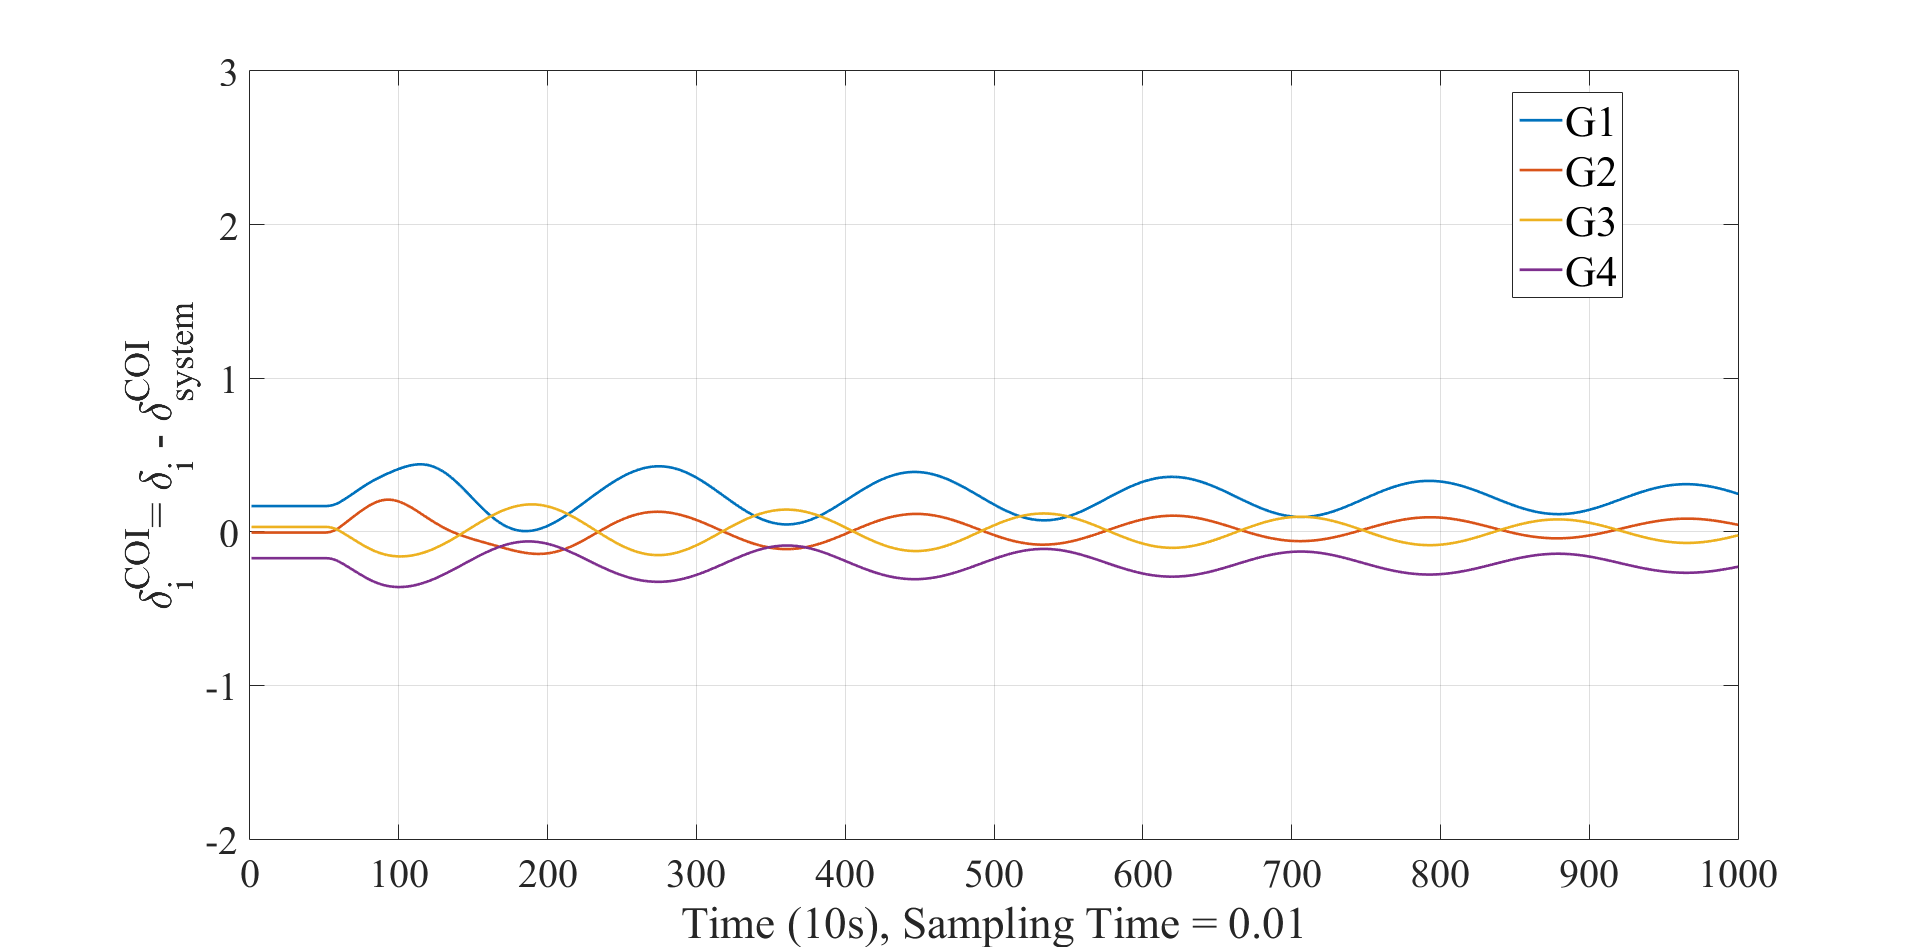
\includegraphics[width=\linewidth]{Co A1}
  \caption{Speed Deviation Vs. Time for \(T_c\) = 0.1 sec}
  \label{fig:I1sub2}
\end{subfigure}
\\
\begin{subfigure}{.5\textwidth}
  \centering
  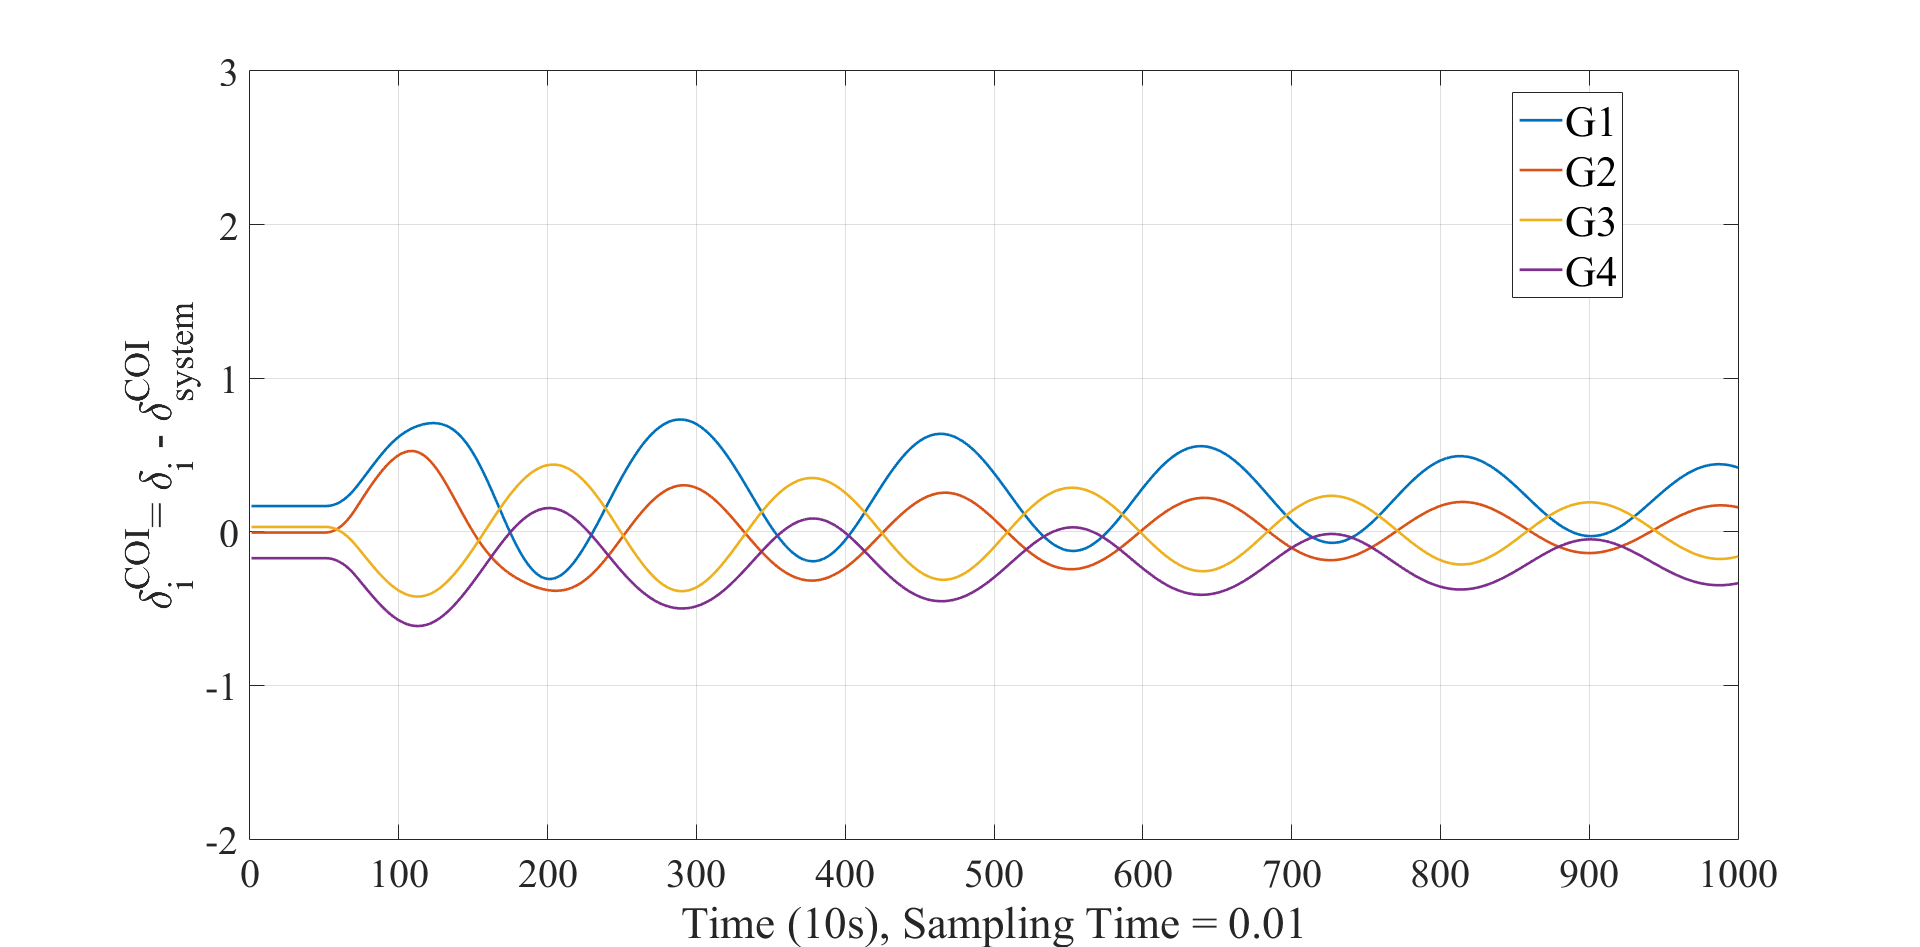
\includegraphics[width=\linewidth]{Co A2}
  \caption{Speed Deviation Vs. Time for \(T_c\) = 0.2 sec}
  \label{fig:I1sub3}
\end{subfigure}%
\begin{subfigure}{.5\textwidth}
  \centering
  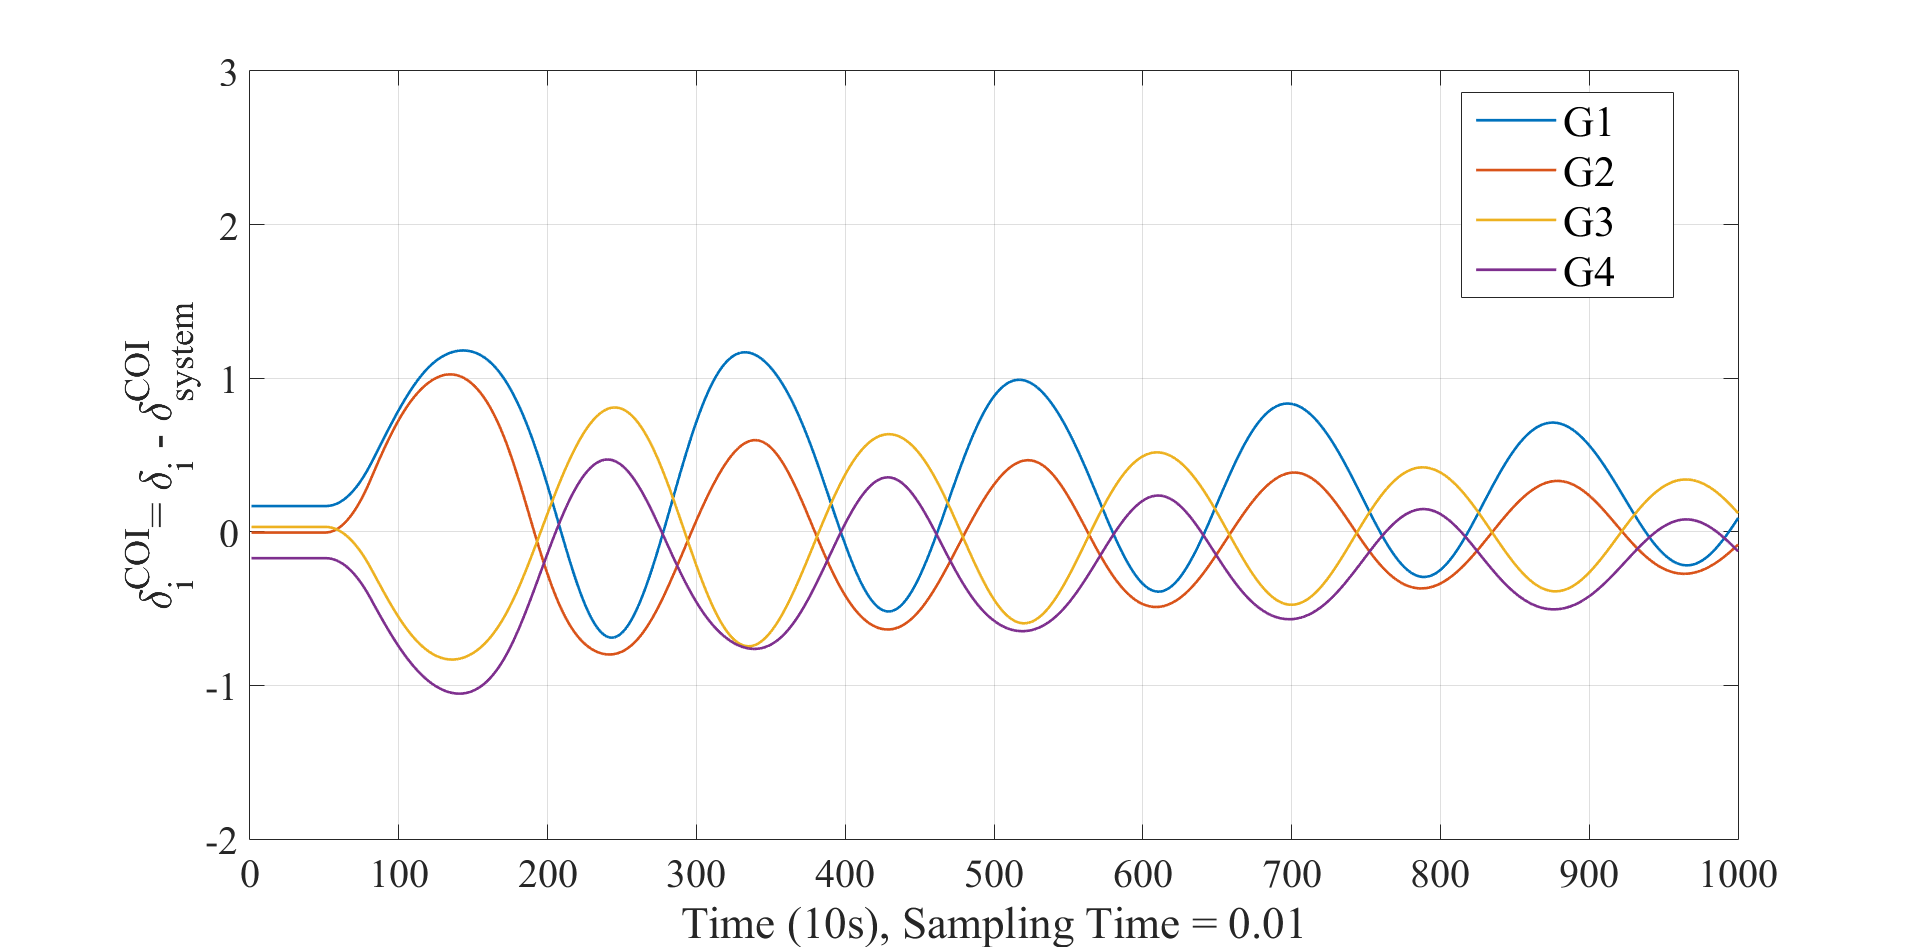
\includegraphics[width=\linewidth]{Co A3}
  \caption{Speed Deviation Vs. Time for \(T_c\) = 0.3 sec}
  \label{fig:I1sub4}
\end{subfigure}
\\
\begin{subfigure}{.5\textwidth}
  \centering
  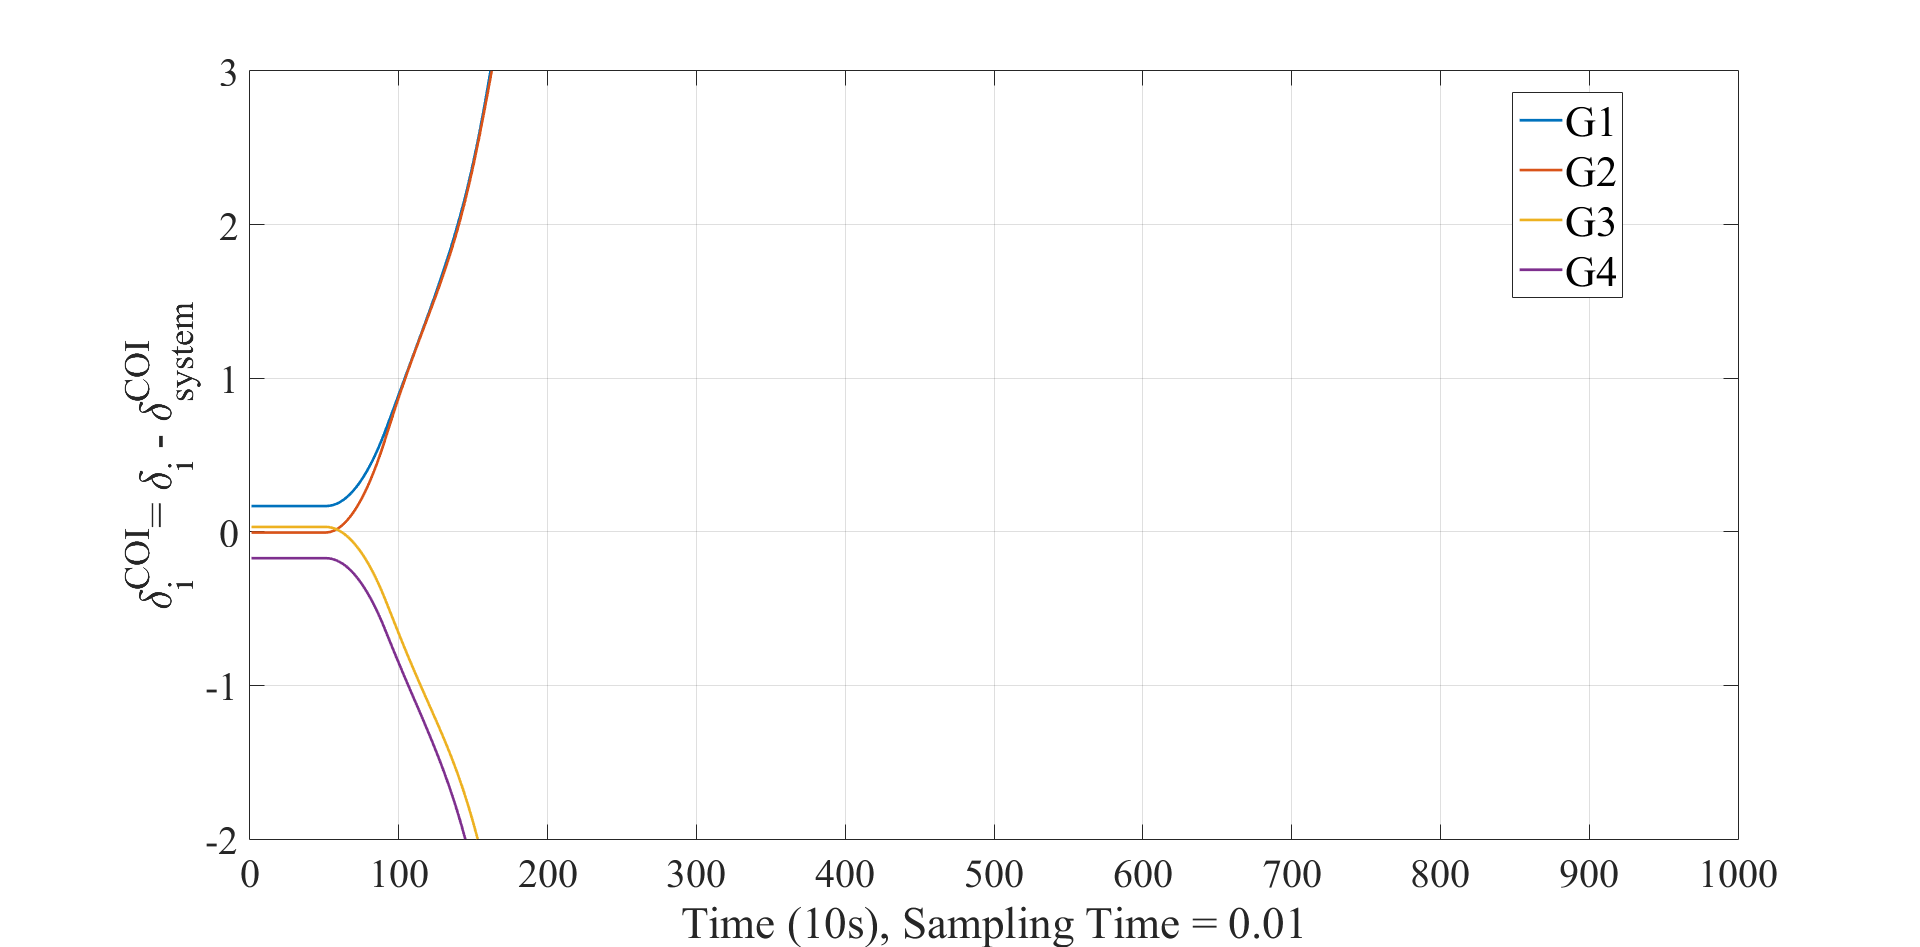
\includegraphics[width=\linewidth]{Co A4}
  \caption{Speed Deviation Vs. Time for \(T_c\) = 0.4 sec}
  \label{fig:I1sub5}
\end{subfigure}
\caption{Indicator based on Coherency}
\label{fig:I1}
\end{figure}

\begin{table}[H]
\renewcommand{\arraystretch}{1}
\caption{Contingency Analysis using Indicator based on Coherency}
\label{Table:I1}
\begin{center}
\begin{tabular}{|P{0.3\linewidth} | P{0.3\linewidth} | P{0.2\linewidth}|}
\hline
 \textbf{Fault Clearing Time} & \textbf{Performance Index} & \textbf{Remarks}  \\ \hline
 No Fault & 1.7262e-10  & Stable \\ \hline
 0.1 sec & 0.4349  & Stable \\ \hline
 0.2 sec & 1.0385  & Stable \\ \hline
 0.3 sec & 1.8697  & Stable \\ \hline
 0.4 sec & 66.9471  & Unstable \\ \hline
 
\end{tabular}
\end{center}
\end{table}




\subsection{Results for Indicator based on Transient Energy Conversion}
\label{Ind2}
\begin{figure}[H]
\centering
\begin{subfigure}{.5\textwidth}
  \centering
  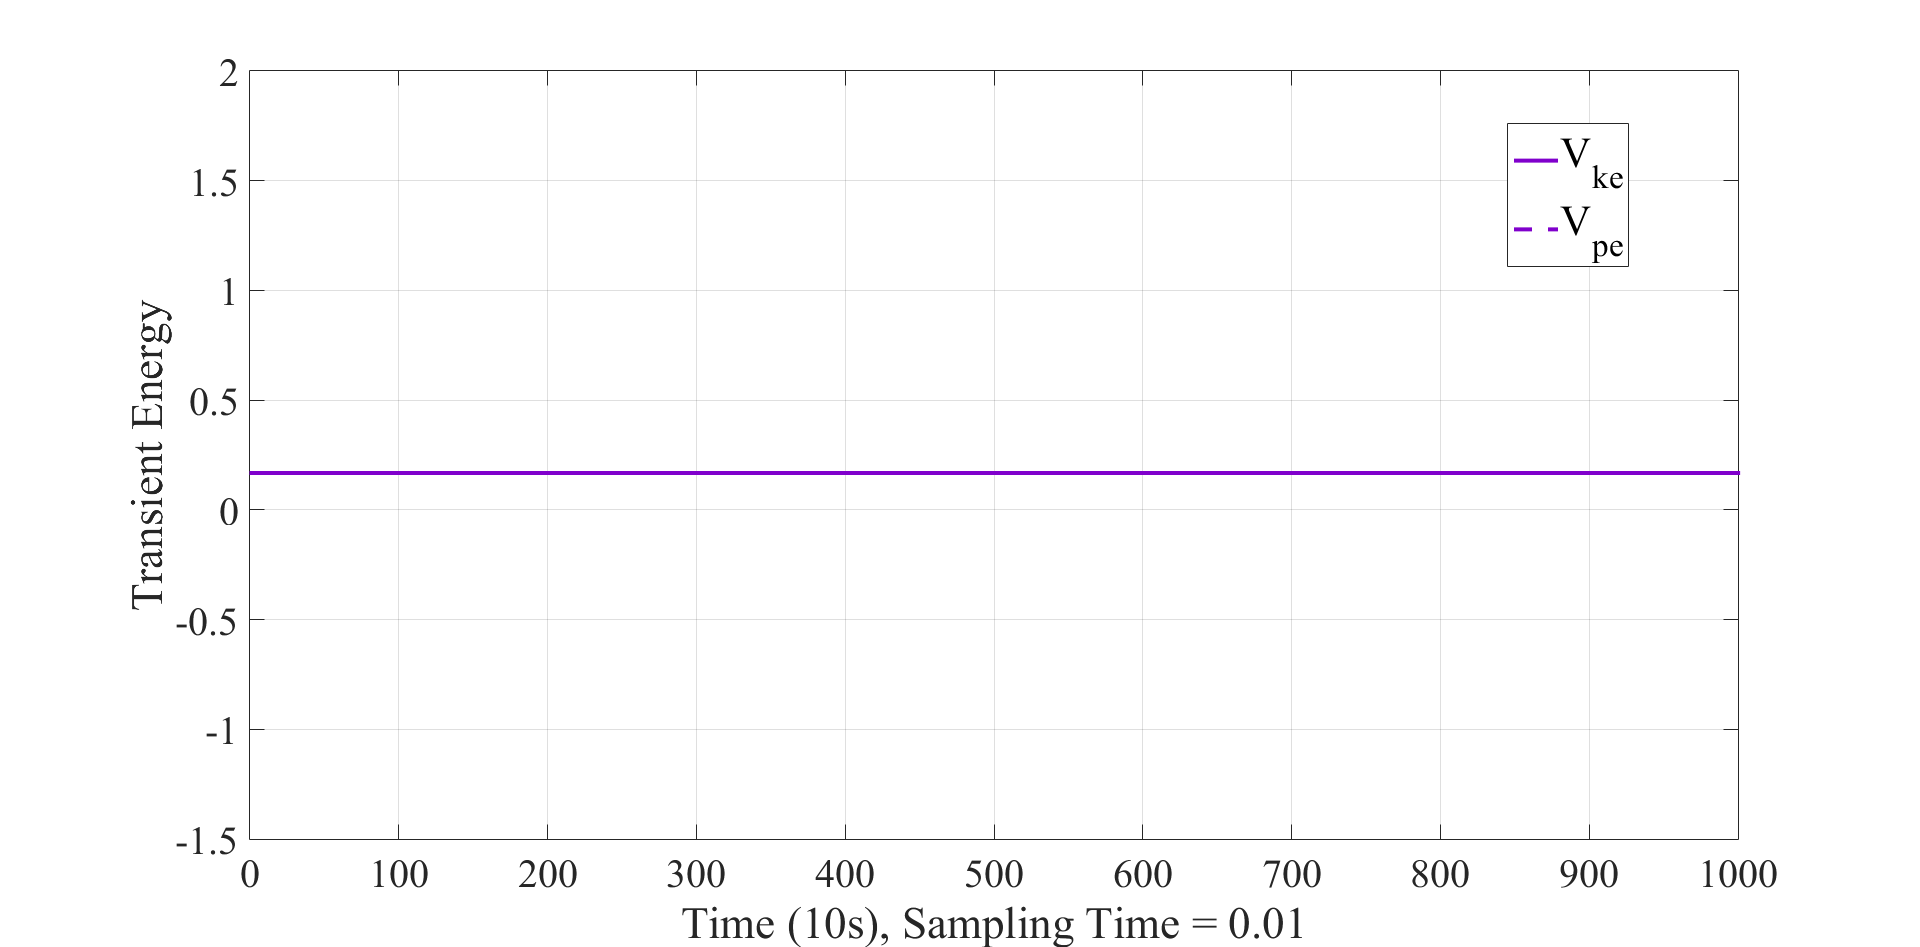
\includegraphics[width=\linewidth]{TE No Fault}
  \caption{Transient Energy Vs. Time for No Fault}
  \label{fig:I2sub1}
\end{subfigure}%
\begin{subfigure}{.5\textwidth}
  \centering
  \includegraphics[width=\linewidth]{TE A1}
  \caption{Transient Energy Vs. Time for \(T_c\) = 0.1 sec}
  \label{fig:I2sub2}
\end{subfigure}
\\
\begin{subfigure}{.5\textwidth}
  \centering
  \includegraphics[width=\linewidth]{TE A2}
  \caption{Transient Energy Vs. Time for \(T_c\) = 0.2 sec}
  \label{fig:I2sub3}
\end{subfigure}%
\begin{subfigure}{.5\textwidth}
  \centering
  \includegraphics[width=\linewidth]{TE A3}
  \caption{Transient Energy Vs. Time for \(T_c\) = 0.3 sec}
  \label{fig:I2sub4}
\end{subfigure}
\\
\begin{subfigure}{.5\textwidth}
  \centering
  \includegraphics[width=\linewidth]{TE A4}
  \caption{Transient Energy Vs. Time for \(T_c\) = 0.4 sec}
  \label{fig:I2sub5}
\end{subfigure}
\caption{Indicator based on Transient Energy Conversion}
\label{fig:I2}
\end{figure}

\begin{table}[H]
\renewcommand{\arraystretch}{1}
\caption{Contingency Analysis using Indicator based on Transient Energy Conversion}
\label{Table:I2}
\begin{center}
\begin{tabular}{|P{0.3\linewidth} | P{0.3\linewidth} | P{0.2\linewidth}|}
\hline
 \textbf{Fault Clearing Time} & \textbf{Performance Index} & \textbf{Remarks}  \\ \hline
 No Fault & 3.3922e-10  & Stable \\ \hline
 0.1 sec & 0.5432  & Stable \\ \hline
 0.2 sec & 1.1266  & Stable \\ \hline
 0.3 sec & 2.0253  & Stable \\ \hline
 0.4 sec & 133.8941  & Unstable \\ \hline
 
\end{tabular}
\end{center}
\end{table}



\subsection{Results for Indicator based on Dot Products (CSA)}
\label{Ind3}
\begin{figure}[H]
  \centering
  \includegraphics[width=\linewidth]{CSA}
  \caption{Contingency Severity Assessment (CSA)}
  \label{fig:I4}


\end{figure}

\begin{table}[H]
\renewcommand{\arraystretch}{1}
\caption{Contingency Analysis using Indicator based on Dot Products (CSA)}
\label{Table:I3}
\begin{center}
\begin{tabular}{|P{0.3\linewidth} | P{0.3\linewidth} | P{0.2\linewidth}|}
\hline
 \textbf{Fault Clearing Time} & \textbf{Performance Index} & \textbf{Remarks}  \\ \hline
 No Fault & 1.5902e-10  & Stable \\ \hline
 0.1 sec & 0.9557  & Stable \\ \hline
 0.2 sec & 3.5214  & Stable \\ \hline
 0.3 sec & 9.6711  & Stable \\ \hline
 0.4 sec & 2.4770e+03  & Unstable \\ \hline
 
\end{tabular}
\end{center}
\end{table}



\subsection{Results for Wide Area Severity Index (WASI)}
\label{Ind4}
\begin{figure}[H]
  \centering
  \includegraphics[width=\linewidth]{WASIcurve}
  \caption{Wide Area Severity Index (WASI)}
  \label{fig:I3}


\end{figure}

\begin{table}[H]
\renewcommand{\arraystretch}{1}
\caption{Contingency Analysis using Wide Area Severity Index (WASI)}
\label{Table:I4}
\begin{center}
\begin{tabular}{|P{0.3\linewidth} | P{0.3\linewidth} | P{0.2\linewidth}|}
\hline
 \textbf{Fault Clearing Time} & \textbf{Performance Index} & \textbf{Remarks}  \\ \hline
 No Fault & -88.4891  & Stable \\ \hline
 0.1 sec & -80.7781  & Stable \\ \hline
 0.2 sec & -68.1678  & Stable \\ \hline
 0.3 sec & -67.3590  & Stable \\ \hline
 0.4 sec & -1.0775  & Unstable \\ \hline
 
\end{tabular}
\end{center}
\end{table}


\subsection{Results for Inter-area Stability Prediction Index (ISPI)}
\label{Ind5}
\begin{table}[H]
\renewcommand{\arraystretch}{1}
\caption{Contingency Analysis using Inter-area Stability Prediction Index (ISPI)}
\label{Table:I5}
\begin{center}
\begin{tabular}{|P{0.3\linewidth} | P{0.3\linewidth} | P{0.2\linewidth}|}
\hline
 \textbf{Fault Clearing Time} & \textbf{ISPI} & \textbf{Remarks}  \\ \hline
 No Fault & 0.0000  & Stable \\ \hline
 0.1 sec & 3.1537  & Stable \\ \hline
 0.2 sec & 11.6207  & Stable \\ \hline
 0.3 sec & 31.9145  & Stable \\ \hline
 0.4 sec & 82.5676  & Unstable \\ \hline
 0.5 sec & 92.5350  & Unstable \\ \hline
 
\end{tabular}
\end{center}
\end{table}

\begin{figure}[H]
  \centering
  \includegraphics[width=\linewidth]{ISPI Bar graph}
  \caption{Inter-area Stability Prediction Index}
  \label{fig:I5}


\end{figure}

\section{Stability Analysis in Other Test Systems}
\label{R_Contingency}

\begin{table}[H]
\renewcommand{\arraystretch}{1}
\caption{Stability Analysis in Different Contingencies}
\label{Table:R_Contingency}
\begin{tabular}{|P{1.9 cm} | P{1.9 cm} | P{1.9 cm}|P{1.9 cm} | P{1.9 cm} | P{1.9 cm}| P{0.6 cm}|}
\hline
  
  \textbf{\textit{Fault Clearance Time}}  & \textbf{Coherency based Indicator} & \textbf{TEC based Indicator} & \textbf{CSA Indicator} & \textbf{WASI Indicator} & \textbf{ISPI Indicator} & \textbf{R*} \\\hline
 
    \bottomrule
    \bottomrule
    \multicolumn{7}{P{14 cm}}{\textit{\textbf{Contingency 1:} \textbf{145}-Bus, \textbf{50}-Machine System  \textbf{||}  Fault on Bus-\textbf{100}  \textbf{||}  Line Tripped between Bus-\textbf{100} and Bus-\textbf{103}}}\\\hline
    
    \textbf{0.1 sec} & 0.7925 & 1.1139 & 6.0352 & -132.6903 & 19.9160 & S\\\hline
    \textbf{0.2 sec} & 1.9300 & 2.3566 & 17.9379 & -81.9617 & 33.3588 & S\\\hline
    \textbf{0.3 sec} & 1.3248e+03 & 2.6497e+03 & 3.7071e+05 & -9.2605 & 100 & U\\\hline
    \textbf{0.4 sec} & 1.3913e+03 & 2.7826e+03 & 3.9845e+05 & -6.9247 & 100 & U\\\hline
     
     \bottomrule
    \multicolumn{7}{P{14 cm}}{\textit{\textbf{Contingency 2:} \textbf{10}-Bus, \textbf{4}-Machine System  \textbf{||}  Fault on Bus-\textbf{8}  \textbf{||}  Line Tripped between Bus-\textbf{7} and Bus-\textbf{8}}}\\\hline
    
    \textbf{0.1 sec} & 0.3341 & 0.6311 & 0.4248 & -78.2523 & 1.4020 & S\\\hline
    \textbf{0.2 sec} & 0.5372 & 0.8180 & 0.7497 & -77.2143 & 2.4740 & S\\\hline
    \textbf{0.3 sec} & 0.8436 & 1.1307 & 1.7686 & -75.2880 & 5.8365 & S\\\hline
    \textbf{0.4 sec} & 1.2719 & 1.2682 & 3.8308 & -63.7517 & 12.6416 & S\\\hline
    \textbf{0.5 sec} & 1.8062 & 2.1298 & 8.9612 & -62.0844 & 29.5719 & S\\\hline
    \textbf{0.6 sec} & 28.7068 & 46.7095 & 317.4158 & -4.7632 & 66.0481 & U\\\hline
    \textbf{0.7 sec} & 38.9884 & 66.7956 & 382.7585 & -1.3148 & 66.0580 & U\\\hline
    
    \bottomrule
    \multicolumn{7}{P{14 cm}}{\textit{\textbf{Contingency 3:} \textbf{145}-Bus, \textbf{50}-Machine System  \textbf{||}  Fault on Bus-\textbf{7}  \textbf{||}  Line Tripped between Bus-\textbf{7} and Bus-\textbf{8}}}\\\hline
    
    \textbf{0.01 sec} & 0.3215 & 0.1923 & 2.2805 & -240.8413
 & 7.5255 & S\\\hline
    \textbf{0.05 sec} & 1.6974 & 0.8372 & 20.5659 & -217.2081 & 33.4113 & S\\\hline
    \textbf{0.1 sec} & 78.1968 & 153.5396 & 6.6780e+03 & -2.7570 & 66.7798 & U\\\hline
    
\end{tabular}
\end{table}
\textbf{* R} - Remarks, \textbf{S} - Stable, \textbf{U} - Unstable

\section{Discussion}
For illustration of applicability of aforementioned catastrophic
indicators 4 contingencies are taken as example in previous sections. The first contingency discussed in section \ref{contingency1} is the IEEE 10 Bus 4 Machine System, in which a fault is applied on Bus 9 and the fault is eliminated by releasing the connection between Bus-9 and Bus-10 at different fault clearing periods. Results of Indicators are analysed through curves (refer Fig. \ref{fig:I1} to Fig. \ref{fig:I4}) as well as in tabular form (refer Fig. \ref{Table:I1} to Fig. \ref{Table:I5}). For Indicator 1 i.e. Indicator based on Coherency results are provided in section \ref{Ind1} shows 5 figures for each Fault Clearing Time including No fault. The data are observed clearly that for no fault and 0.1 sec, 0.2 sec and 0,3 sec the curves of generator speed are deviating gradually but in 0.4 sec there is larger deviation and its peak is at 66.9471 p.u. i.e Performance Index for 1st Indicator where as PI (Performance index) is very much small in other four Tclear times. Similar situation in Indicator 2 i.e. Indicator based on Transient Energy Conversion (refer section \ref{Ind2}), Performance Index for 0.4 sec Tclear is 133.8941, where as for other four cases it is less than 3 p.u. The difference between Kinetic and potential energy is much higher for Tclear =0.4 sec. So, it is obvious that system is not in stable state. In section \ref{Ind3} third Indicator i.e. Indicator based on Dot Products (CSA)
results are defined and its in single curve because the PI is produced in single curve (refer fig. \ref{fig:I3}). For each Tclear time one curve of specific color is drawn from algorithm for the taken contingency and the reference color data can be guided from legend provided on curve. From the curve can also one can distinguish between stable and unstable cases. The deviation here is also refers the Performance Index. Its tabular data shows the deviation upto Tclear 0.3 sec starting from No fault is 9.6711 and on 0.4 sec Tclear it reaches to 2.4770e+03. These 3 indicators posses same pattern and all are clearly indicating the system condition. The large gap in numbers and in curves itself is the proof of Indicator working. Its not always not possible to plot each and every system in plots because of high power ratings, so, indicator 4 i.e. Wide Area Severity Index (WASI) (results are discussed in section \ref{Ind4}). As it is in logarithmic form so higher values are compressed to minimum value possible so it is each to observe through machines. The PI of WASI is different from discussed above 3 methods and it is observed that result occurs in -y axis. But similar to them, here also there is large difference in values between stable and unstable condition. Fifth Indicator i.e. Inter-area Stability Prediction Index (ISPI) (results are discussed in section \ref{Ind5}) produces results in percentage and it is previously defined in section \ref{ISPI_Intro} that for how much percentage the system is stable and for what it is unstable. Now the data are produced in both tabular and graphical form manually collected from algorithm and observed that for Tclear 0.3 sec and below the PI is below 33\% and for Tclear = 0.4 sec the PI is 82.5676\%, which is in alarming state. So, both the data(Graphical as well as Tabular) shows for Tclear = 0.1 sec, 0.2 sec, 0.3 sec the system behaves stable performance after fault, but for Tclear = 0.4 sec system moves to unstable state. So, the Threshold Tclear lies between 0.3 sec and 0.4 sec and it is found to be 0.318 sec when it is executed manually. Analysis of Indicator states that all the Indicator has different Threshold values (not Threshold Tclear). Similarly in section \ref{R_Contingency} other three contingencies are performed for Indicator Analysis. The Indicator performances are described in Table \ref{Table:R_Contingency}, the results (behaviour of the system, i.e. Stable or Unstable) for all the aforementioned catastrophic indicators are same for a particular value of Tclear.
 % Results and Discussion
\chapter{Conclusion and Future Scope}
\section{Conclusion}
This project effort gives several indices for security analysis contingency screening. Again after disturbance has been addressed, these indicators are focused on coherency, transient energy conversion between kinetic and potential energy, dot products, and generator coupling parameters. These indices are quick to calculate because they don't require a lengthy simulation to determine if a situation is stable or unstable. They are precise because they have a high probability of capturing all unstable circumstances. These indices have been examined on a variety of test systems in the background while developing project including the discussed contingencies, and the findings indicate that the result provided by each of the indicator is correct and match to the original data. The possibility of mis-detection is zero till now, so this could be useful in future contingency screening.

 \pagebreak

\section{Future Scope}


The Catastrophic indicators have been analysed through a single method i.e. observing sudden rise in the curve to analyse the system behaviour in my paper. But there is need to define Threshold values for each indicator to observe the system behaviour after fault. Finding Threshold values through any type of optimization method or any other makes this Indicator Evaluation a complete process. In \cite{8}, the age of the possibility dataset and the calculation of execution allots are communicated via MATLAB in both offline and web-based modes. High-performance computing (HPC) \cite{FR1} or equal handling engineering \cite{FR2}, which is one of the conceivable forthcoming bearings identified, can be used to construct an internet-based structure.

 % Conclusion



\addtocontents{toc}{\vspace{2em}} % Add a gap in the Contents, for aesthetics

\endgroup

\backmatter

\cleardoublepage
\begin{thebibliography}{99}
\begin{singlespace}
% Introductory
\bibitem{SAPS} B. Shakerighadi, S. Peyghami, E. Ebrahimzadeh, F. Blaabjerg and C. Leth Back, "A New Guideline for Security Assessment of Power Systems with a High Penetration of Wind Turbines," \textit{Applied Sciences}, vol. 10, no. 9, pp. 3190-3206, 2020.

\bibitem{I6} A. Mittal, J. Hazra, N. Jain, V. Goyal, D. Seetharam and Y. Sabharwal, "Real Time Contingency Analysis for Power Grids," in \textit{Proc. European Conference on Parallel Processing}, pp. 303-315, 2011, Berlin, Heidelberg.


%Literature Survey
\bibitem{L1} R. Zimmerman, C. Murillo-Sanchez and R. Thomas, "MATPOWER: Steady-State Operations, Planning, and Analysis Tools for Power Systems Research and Education," \textit{IEEE Transactions on Power Systems}, vol. 26, no. 1, pp. 12-19, 2011.
% previously
\bibitem{L2} H. Yang, K. Niu, D. Xu and S. Xu, "Analysis of power system transient stability characteristics with the application of massive transient stability simulation data," \textit{Energy Reports}, vol. 7, pp. 111-117, 2021. 

\bibitem{L3} I. Genc, Ruisheng Diao and V. Vittal, "Computation of transient stability related security regions and generation rescheduling based on decision trees," in \textit{Proc. IEEE PES General Meeting}, pp. 1-6, 25-29 July 2010, Minneapolis, MN, USA.

\bibitem{L4} L. Wehenkel, "Decision tree approach to power systems security assessment," \textit{International Journal of Electrical Power \& Energy Systems}, vol. 15, no. 1, pp. 13-36, 1993.

\bibitem{L5} L. Wehenkel and M. Pavella, "Decision trees and transient stability of electric power systems," \textit{Automatica}, vol. 27, no. 1, pp. 115-134, 1991. 
% ----------------
\bibitem{L6} Y. Zhang, W. Liu, Y. Huan, Q. Zhou and N. Wang, "Online Dynamic Total Transfer Capability Estimation Using Cotraining-Style Semi-Supervised Regression," \textit{IEEE Access}, vol. 8, pp. 94054-94064, 2020.

\bibitem{L7} S. Jafarzadeh, I. Genc and A. Nehorai, "Real-time transient stability prediction and coherency identification in power systems using Koopman mode analysis," \textit{Electric Power Systems Research}, vol. 201, pp. 107565-107577, 2021.

\bibitem{L8} M. Teixeira, I. Melo and J. Filho, "An optimisation model based approach for power systems voltage stability and harmonic analysis," \textit{Electric Power Systems Research}, vol. 199, pp. 107462-107473, 2021.

\bibitem{L9} L. Meegahapola, S. Bu, D. Wadduwage, C. Chung and X. Yu, "Review on Oscillatory Stability in Power Grids With Renewable Energy Sources: Monitoring, Analysis, and Control Using Synchrophasor Technology," \textit{IEEE Transactions on Industrial Electronics}, vol. 68, no. 1, pp. 519-531, 2021.

\bibitem{L10} Y. Chompoobutrgool, L. Vanfretti and M. Ghandhari, "Survey on power system stabilizers control and their prospective applications for power system damping using Synchrophasor-based wide-area systems," \textit{European Transactions on Electrical Power}, vol. 21, no. 8, pp. 2098-2111, 2011.

\bibitem{L11} S. Ghaedi, S. Abazari and G. Arab Markadeh, "Transient stability improvement of power system with UPFC control by using transient energy function and sliding mode observer based on locally measurable information," \textit{Measurement}, vol. 183, pp. 109842-109854, 2021. Available: 10.1016/j.measurement.2021.109842

\bibitem{L12} A. Sobbouhi and A. Vahedi, "Transient stability prediction of power system; a review on methods, classification and considerations," \textit{Electric Power Systems Research}, vol. 190, pp. 106853-106869, 2021.

\bibitem{L13} I. Kamwa, S. Samantaray and G. Joos, "Catastrophe Predictors From Ensemble Decision-Tree Learning of Wide-Area Severity Indices," \textit{IEEE Transactions on Smart Grid}, vol. 1, no. 2, pp. 144-158, 2010.

\bibitem{L15} W. Villa-Acevedo, J. López-Lezama, D. Colomé and J. Cepeda, "Long-term voltage stability monitoring of power system areas using a kernel extreme learning machine approach," \textit{Alexandria Engineering Journal}, vol. 61, no. 2, pp. 1353-1367, 2022.


% for print
%
%\bibitem{L2} H. Yang, K. Niu, D. Xu and S. Xu, "Analysis of power system transient stability characteristics with the application of massive transient stability simulation data," \textit{Energy Reports}, vol. 7, pp. 111-117, 2021. 
%
%\bibitem{L3} I. Genc, Ruisheng Diao and V. Vittal, "Computation of transient stability related security regions and generation rescheduling based on decision trees," in \textit{Proc. IEEE PES General Meeting}, pp. 1-6, 25-29 July 2010, Minneapolis, MN, USA.
%
%\bibitem{L4} L. Wehenkel, "Decision tree approach to power systems security assessment," \textit{International Journal of Electrical Power \& Energy Systems}, vol. 15, no. 1, pp. 13-36, 1993.
%
%\bibitem{L5} L. Wehenkel and M. Pavella, "Decision trees and transient stability of electric power systems," \textit{Automatica}, vol. 27, no. 1, pp. 115-134, 1991. 



% Project Motivation

\bibitem{1} S. Abhyankar, G. Geng, M. Anitescu, X. Wang and V. Dinavahi, "Solution techniques for transient stability‐constrained optimal power flow – Part I," \textit{IET Generation, Transmission \& Distribution}, vol. 11, no. 12, pp. 3177-3185, 2017.

\bibitem{2} G. Geng, S. Abhyankar, X. Wang and V. Dinavahi, "Solution techniques for transient stability‐constrained optimal power flow – Part II," \textit{IET Generation, Transmission \& }; Distribution, vol. 11, no. 12, pp. 3186-3193, 2017.

\bibitem{5} A. Sobbouhi and A. Vahedi, "Online synchronous generator out-of-step prediction by ellipse fitting on acceleration power – Speed deviation curve," \textit{International Journal of Electrical Power \& Energy Systems}, vol. 119, pp. 105965-105973, 2020.

\bibitem{I5} A. Sobbouhi and A. Vahedi, "Transient stability improvement based on out-of-step prediction," \textit{Electric Power Systems Research}, vol. 194, pp. 107108-107119, 2021.
%%%%%%%%%%%%%%%%
\bibitem{I3} M. Mynuddin, "Stability Study of Power System," \textit{International Journal of Energy and Power Engineering}, vol. 4, no. 2, pp. 43-51, 2015.

\bibitem{7} P. Kundur, N. J Balu and M. G Lauby, \textit{Power system stability and control}, 7th ed. Electrical Power Research Institute, New York: McGraw-Hill Professional, 1994.

\bibitem{8} G. Ravikumar and S. Khaparde, "Taxonomy of PMU Data Based Catastrophic Indicators for Power System Stability Assessment," \textit{IEEE Systems Journal}, vol. 12, no. 1, pp. 452-464, 2018.

\bibitem{9} H. Hashim, I. Abidin, H. Rashid, N. Zulkapli, S. Ibrahim, S. Kamar and N. Sofizan, "An out-of-step detection based on transient stability index," \textit{Aust. J. Basic Appl. Sci.}, vol. 7, no. 4, pp. 353-365, 2013.
%
\bibitem{EPM} C. Fu and A. Bose, "Contingency ranking based on severity indices in dynamic security analysis," \textit{IEEE Transactions on Power Systems}, vol. 14, no. 3, pp. 980-985, 1999. Available: 10.1109/59.780910
%
\bibitem{CSA} I. Kamwa, R. Grondin and L. Loud, "Time-varying contingency screening for dynamic security assessment using intelligent-systems techniques," \textit{IEEE Transactions on Power Systems}, vol. 16, no. 3, pp. 526-536, 2001.
%
\bibitem{CSA_WASI} I. Kamwa, S. Samantaray and G. Joos, "Development of Rule-Based Classifiers for Rapid Stability Assessment of Wide-Area Post-Disturbance Records," \textit{IEEE Transactions on Power Systems}, vol. 24, no. 1, pp. 258-270, 2009.

\bibitem{ISPI} O. Gomez and M. Rios, "Inter-area stability prediction index based on phasorial measurement," in \textit{Proc. IEEE PES Innovative Smart Grid Technologies (ISGT)}, pp. 1-8, 16-20 Jan. 2012, Washington, DC, USA.
%
\bibitem{MattransSoft} G. Ravikumar, "\textit{MATTRANS: a MATLAB power system transient stability simulation package}", 2016. [Online]. Available: https://github.com/gelliravi/MatTrans.
%
\bibitem{FR1} R. Green, L. Wang and M. Alam, "High performance computing for electric power systems: Applications and trends," in \textit{Proc. IEEE Power and Energy Society General Meeting}, pp. 1-8, 24-28 July 2011, Detroit, MI, USA.
%
\bibitem{FR2} V. Jalili-Marandi, Zhiyin Zhou and V. Dinavahi, "Large-scale transient stability simulation of electrical power systems on parallel GPUs," in \textit{Proc. IEEE Power and Energy Society General Meeting}, pp. 1-11, 22-26 July 2012, San Diego, CA, USA.
%
%
%
%\bibitem{}
%
%\bibitem{}
%
%\bibitem{}
%
%\bibitem{}
%
%\bibitem{}
%
%\bibitem{}
%
%\bibitem{}
%
%\bibitem{}
%
%\bibitem{}
%
%\bibitem{}
%
%\bibitem{}
%
%\bibitem{}
%
%\bibitem{}
\end{singlespace}

\end{thebibliography} % References




\end{document}